\documentclass[a4paper,11pt,twoside]{memoir}
\chapterstyle{plain}

\usepackage{TUINFDA}

\usepackage{url}
\usepackage{hyperref}					% links in pdf
\usepackage{graphicx}            			% Figures
\usepackage{interval}
\usepackage{verbatim}            			% Code-Environment
\usepackage[lined,linesnumbered,algochapter]{algorithm2e} % Algorithm-Environment
\newsubfloat{figure}
\newsubfloat{table}

\usepackage{booktabs}
\usepackage{pgf}					
\usepackage{tikz}					% tikz graphics
\usetikzlibrary{arrows,automata}
\usepackage{pgfplots}
\usepackage{pgfplotstable}
\usepackage{colortbl}
\pgfplotsset{compat=newest}
\usepgfplotslibrary{groupplots}
\usetikzlibrary{pgfplots.groupplots}
%\usetikzlibrary{external}
\usetikzlibrary{matrix}
\usetikzlibrary{spy}
%\tikzexternalize[prefix=tikz/]
%\tikzset{external/up to date check=md5}

\usepackage{ngerman}
\usepackage[ngerman]{babel}
\usepackage{bibgerm,cite}       % Deutsche Bezeichnungen, Automatisches Zusammenfassen von Literaturstellen
\usepackage[ngerman]{varioref}  % Querverweise
% to use the german charset include cp850 for MS-DOS, ansinew for Windows and latin1 for Linux.
% \usepackage[latin1]{inputenc}
\usepackage{mathtools}
\usepackage{array}
\usepackage{multirow}
\usepackage{siunitx}
\usepackage{commath}
\usepackage{hhline}
\usepackage[sectionbib]{natbib}
\usepackage{csvsimple}

\DeclareSIUnit\pixel{px}

\DeclarePairedDelimiter{\ceil}{\lceil}{\rceil}
\DeclarePairedDelimiter{\floor}{\lfloor}{\rfloor}
\newcommand{\mvec}[1]{\mathbf{#1}}
\newcommand{\mvecx}[1]{\mathbf{#1}_x}
\newcommand{\mvecy}[1]{\mathbf{#1}_y}
\newcommand{\mvecz}[1]{\mathbf{#1}_z}
\newcommand{\mvecw}[1]{\mathbf{#1}_w}
\newcommand{\mmat}[1]{\mathbf{#1}}
\newcommand{\transpose}[1]{#1^{\mathsf{T}}}
\newcommand{\inverse}[1]{#1^{\mathsf{-1}}}
\newcommand{\normalise}[1]{\frac{#1}{\norm{#1}}}

\newcommand{\wavevector}{wavevector\xspace}
\newcommand{\wavevectors}{wavevectors\xspace}
\newcommand{\Wavevector}{Wavevector\xspace}
\newcommand{\Wavevectors}{Wavevectors\xspace}
\newcommand{\wavenumber}{wavenumber\xspace}
\newcommand{\wavenumbers}{wavenumbers\xspace}
\newcommand{\Wavenumber}{Wavenumber\xspace}
\newcommand{\Wavenumbers}{Wavenumbers\xspace}
\newcommand{\wavelength}{wavelength\xspace}
\newcommand{\wavelengths}{wavelengths\xspace}
\newcommand{\Wavelength}{Wavelength\xspace}
\newcommand{\Wavelengths}{Wavelengths\xspace}

\newcommand{\FourierTransform}{Fourier Transform\xspace}
\newcommand{\FourierTransforms}{Fourier Transforms\xspace}
\newcommand{\InvFourierTransform}{Inverse Fourier Transform\xspace}
\newcommand{\InvFourierTransforms}{Inverse Fourier Transforms\xspace}
\newcommand{\DiscreteFourierTransform}{Discrete Fourier Transform\xspace}
\newcommand{\DiscreteFourierTransforms}{Discrete Fourier Transforms\xspace}
\newcommand{\InvDiscreteFourierTransform}{Inverse Discrete Fourier Transform\xspace}
\newcommand{\InvDiscreteFourierTransforms}{Inverse Discrete Fourier Transforms\xspace}
\newcommand{\FastFourierTransform}{Fast Fourier Transform\xspace}
\newcommand{\FastFourierTransforms}{Fast Fourier Transforms\xspace}
\newcommand{\FT}{FT\xspace}
\newcommand{\IFT}{IFT\xspace}
\newcommand{\DFT}{DFT\xspace}
\newcommand{\IDFT}{IDFT\xspace}
\newcommand{\IDFTs}{IDFTs\xspace}
\newcommand{\FFT}{FFT\xspace}

\thesistitle{Ocean Surface Generation and Rendering}
%\thesissubtitle{Optional Subtitle} % optional
\thesisdate{11.07.2018}

% all titles and designations have to be gender-related!
\thesisdegree{Diplom-Ingenieur}{Diplom-Ingenieur}
\thesiscurriculum{Visual Computing}{Visual Computing} % your study
\thesisverfassung{Verfasser} % Verfasser
\thesisauthor{Thomas Gamper} % your name
\thesisauthoraddress{Lehmanngasse 25/2/12, 1230 Wien} % your address
\thesismatrikelno{0107543} % your registration number

\thesisbetreins{Associate Prof. Dipl.-Ing. Dipl.-Ing. Dr.techn. Michael Wimmer}
\thesisbetrzwei{}
%\thesisbetrdrei{Dr. Vorname Familienname} % optional

% define page numbering styles
\makepagestyle{numberCorner}
\makeevenfoot{numberCorner}{\thepage}{}{}
\makeoddfoot{numberCorner}{}{}{\thepage}

% define custom macros for specific formats or names
\newcommand{\uml}[1]{\texttt{#1}}
\newcommand{\cd}{\textsf{Class Diagram}}

\DeclareMathOperator{\sech}{sech}

\intervalconfig{
soft open fences,
}

\renewcommand{\thesection}{\arabic{section}}
\makeatletter
\let\l@section\l@chapter
\makeatother

\begin{document}
\captionnamefont{\bfseries}

%%%%%%%%%%%%%%%%%%%%%%%%%%%%%%%%%%%%%%%%%
%%%   FRONTMATTER    %%%%%%%%%%%%%%%%%%%%
%%%%%%%%%%%%%%%%%%%%%%%%%%%%%%%%%%%%%%%%%
%\frontmatter
\pagenumbering{roman}

%%%%%%%%%%%%%%%%%%%%%%%%%%%%%%%%%%%%%%%%%
%%%   TITLEPAGES    %%%%%%%%%%%%%%%%%%%%%
%%%%%%%%%%%%%%%%%%%%%%%%%%%%%%%%%%%%%%%%%

% the german title page is required as first page
% $Id: titlepage.tex 1752 2010-03-20 11:07:02Z tkren $
%
% TU Wien - Faculty of Informatics
% thesis titlepage
%
% This titlepage is using the geometry package, see
% <http://www.ctan.org/macros/latex/contrib/geometry/geometry.pdf>
%
% For questions and comments send an email to
% Thomas Krennwallner <tkren@kr.tuwien.ac.at>
% or to Petra Brosch <brosch@big.tuwien.ac.at>
%

\selectlanguage{ngerman}

% setup page dimensions for titlepage
\newgeometry{left=2.4cm,right=2.4cm,bottom=2.5cm,top=2cm}

% force baselineskip and parindent
\newlength{\tmpbaselineskip}
\setlength{\tmpbaselineskip}{\baselineskip}
\setlength{\baselineskip}{13.6pt}
\newlength{\tmpparindent}
\setlength{\tmpparindent}{\parindent}
\setlength{\parindent}{17pt}

% first titlepage
\thispagestyle{tuinftitlepage}

%
% Kludge: for each titlepage set \pagenumbering to a different
% style. This is used to fix a problem with hyperref, because there
% are multiple "page 1" and hyperref hates that
%
\pagenumbering{Alph}

\begin{center}
{\ \vspace{3.4cm}}

\begin{minipage}[t][2.8cm][s]{\textwidth}%
\centering
\thesistitlefontHUGE\sffamily\bfseries\tuinfthesistitle\\
\bigskip
{\thesistitlefonthuge\sffamily\bfseries\tuinfthesissubtitle}
\end{minipage}

\vspace{1.3cm}

{\thesistitlefontLARGE\sffamily \tuinfthesistype}

\vspace{6mm}

{\thesistitlefontlarge\sffamily zur Erlangung des akademischen Grades}

\vspace{6mm}

{\thesistitlefontLARGE\sffamily\bfseries \tuinfthesisdegree}

\vspace{6mm}

{\thesistitlefontlarge\sffamily im Rahmen des Studiums}

\vspace{6mm}

{\thesistitlefontLarge\sffamily\bfseries \tuinfthesiscurriculum}

\vspace{6.5mm}

{\thesistitlefontlarge\sffamily eingereicht von}

\vspace{6mm}

{\thesistitlefontLarge\sffamily\bfseries \tuinfthesisauthor}

\vspace{1.5mm}

{\thesistitlefontlarge\sffamily Matrikelnummer \tuinfthesismatrikelno} 

\vspace{1.4cm}

\vspace{0pt}\raggedright\thesistitlefontnormalsize\sffamily
\begin{minipage}[t][1.6cm][t]{\textwidth}%
  %
  an der

  Fakult\"{a}t f\"{u}r Informatik der Technischen Universit\"{a}t Wien
\end{minipage}

\begin{minipage}[t][4cm][t]{\textwidth}%
  \vspace{0pt}\raggedright\thesistitlefontnormalsize\sffamily
  %
  \begin{tabbing}%
	    \hspace{19mm} \= \hspace{66mm} \kill
	    \tuinfthesisbetreuung: \> \tuinfthesisbetreins\\
	    Mitwirkung: \> \tuinfthesisbetrzwei\\
	                \> \tuinfthesisbetrdrei
  \end{tabbing}
\end{minipage}

\begin{minipage}[t][1.5cm][t]{\textwidth}%
  \vspace{0pt}\sffamily\thesistitlefontnormalsize
  \begin{tabbing}%
    \hspace{45mm} \= \hspace{63mm} \= \hspace{51mm} \kill
    Wien, \tuinfthesisdate \> {\raggedright\rule{51mm}{0.5pt}} \> {\raggedright\rule{51mm}{0.5pt}} \\
    \> \begin{minipage}[t][0.5cm][t]{51mm}\centering (Unterschrift \tuinfthesisverfassung)\end{minipage}
    \> \begin{minipage}[t][0.5cm][t]{51mm}\centering (Unterschrift \tuinfthesisbetreuung)\end{minipage}
    \end{tabbing}
\end{minipage}

\end{center}

% we want an empty page right after first titlepage
\pagestyle{empty}
\cleardoublepage

% we're done with the titlepages, proceed with default pagenumbering
\pagenumbering{roman}

% restore baselineskip
\setlength{\baselineskip}{\tmpbaselineskip}
\setlength{\parindent}{\tmpparindent}

% back to normal geometry
\restoregeometry

\selectlanguage{english}

%%% Local Variables:
%%% TeX-PDF-mode: t
%%% TeX-debug-bad-boxes: t
%%% TeX-parse-self: t
%%% TeX-auto-save: t
%%% reftex-plug-into-AUCTeX: t
%%% End:


% an english translation may follow
%% $Id: titlepage.tex 1752 2010-03-20 11:07:02Z tkren $
%
% TU Wien - Faculty of Informatics
% thesis titlepage
%
% This titlepage is using the geometry package, see
% <http://www.ctan.org/macros/latex/contrib/geometry/geometry.pdf>
%
% For questions and comments send an email to
% Thomas Krennwallner <tkren@kr.tuwien.ac.at>
% or to Petra Brosch <brosch@big.tuwien.ac.at>
%

% setup page dimensions for titlepage
\newgeometry{left=2.4cm,right=2.4cm,bottom=2.5cm,top=2cm}

% force baselineskip and parindent
%\newlength{\tmpbaselineskip}
%\setlength{\tmpbaselineskip}{\baselineskip}
%\setlength{\baselineskip}{13.6pt}
%\newlength{\tmpparindent}
%\setlength{\tmpparindent}{\parindent}
%\setlength{\parindent}{17pt}

% first titlepage
\thispagestyle{tuinftitlepage}

%
% Kludge: for each titlepage set \pagenumbering to a different
% style. This is used to fix a problem with hyperref, because there
% are multiple "page 1" and hyperref hates that
%
\pagenumbering{Roman}

\begin{center}
{\ \vspace{3.4cm}}

\begin{minipage}[t][2.8cm][s]{\textwidth}%
\centering
\thesistitlefontHUGE\sffamily\bfseries\tuinfthesistitle\\
\bigskip
{\thesistitlefonthuge\sffamily\bfseries\tuinfthesissubtitle}
\end{minipage}

\vspace{1.3cm}

{\thesistitlefontLARGE\sffamily \tuinfthesistypeen}

\vspace{6mm}

{\thesistitlefontlarge\sffamily submitted in partial fulfillment of the requirements for the degree of}

\vspace{6mm}

{\thesistitlefontLARGE\sffamily\bfseries \tuinfthesisdegreeen}

\vspace{6mm}

{\thesistitlefontlarge\sffamily in}

\vspace{6mm}

{\thesistitlefontLarge\sffamily\bfseries \tuinfthesiscurriculumen}

\vspace{6.5mm}

{\thesistitlefontlarge\sffamily by}

\vspace{6mm}

{\thesistitlefontLarge\sffamily\bfseries \tuinfthesisauthor}

\vspace{1.5mm}

{\thesistitlefontlarge\sffamily Registration Number \tuinfthesismatrikelno} 

\vspace{1.4cm}

\begin{minipage}[t][1.6cm][t]{\textwidth}%
  \vspace{0pt}\raggedright\thesistitlefontnormalsize\sffamily
  %
  to the Faculty of Informatics 

  at the Vienna University of Technology
\end{minipage}

\vspace{0pt}\raggedright\thesistitlefontnormalsize\sffamily
\begin{minipage}[t][4cm][t]{\textwidth}%
  \begin{tabbing}%
	    \hspace{19mm} \= \hspace{66mm} \kill
	    Advisor: \> \tuinfthesisbetreins\\
%	    Assistance: \> \tuinfthesisbetrzwei\\
%	                \> \tuinfthesisbetrdrei
     \end{tabbing}
\end{minipage}

\begin{minipage}[t][1.5cm][t]{\textwidth}%
  \vspace{0pt}\sffamily\thesistitlefontnormalsize
  \begin{tabbing}%
    \hspace{45mm} \= \hspace{63mm} \= \hspace{51mm} \kill
    Vienna, \tuinfthesisdate \> {\raggedright\rule{51mm}{0.5pt}} \> {\raggedright\rule{51mm}{0.5pt}} \\
    \> \begin{minipage}[t][0.5cm][t]{51mm}\centering (Signature of Author)\end{minipage}
    \> \begin{minipage}[t][0.5cm][t]{51mm}\centering (Signature of Advisor)\end{minipage}
    \end{tabbing}
\end{minipage}

\end{center}

% we want an empty page right after first titlepage
\pagestyle{empty}
\cleardoublepage

% we're done with the titlepages, proceed with default pagenumbering
\pagenumbering{roman}

% restore baselineskip
\setlength{\baselineskip}{\tmpbaselineskip}
\setlength{\parindent}{\tmpparindent}

% back to normal geometry
\restoregeometry


%%% Local Variables:
%%% TeX-PDF-mode: t
%%% TeX-debug-bad-boxes: t
%%% TeX-parse-self: t
%%% TeX-auto-save: t
%%% reftex-plug-into-AUCTeX: t
%%% End:
 % optional

%%%%%%%%%%%%%%%%%%%%%%%%%%%%%%%%%%%%%%%%%
%%%   ERKLAERUNG DER SELBSTAENDIGKEIT   %
%%%%%%%%%%%%%%%%%%%%%%%%%%%%%%%%%%%%%%%%%
%\cleardoublepage
%\selectlanguage{ngerman}
%\chapter*{Erklärung zur Verfassung der Arbeit}

\tuinfthesisauthor\\
\tuinfthesisauthoraddress

\vspace*{1.2cm}

Hiermit erkläre ich, dass ich diese Arbeit selbständig verfasst habe, 
dass ich die verwendeten Quellen und Hilfsmittel vollständig angegeben 
habe und dass ich die Stellen der Arbeit - einschließlich Tabellen, 
Karten und Abbildungen -, die anderen Werken oder dem Internet im 
Wortlaut oder dem Sinn nach entnommen sind, auf jeden Fall unter Angabe 
der Quelle als Entlehnung kenntlich gemacht habe.\\

\vspace*{2cm}
\begin{tabbing}%
    \hspace{58mm} \= \hspace{28mm} \= \hspace{58mm} \kill
    {\raggedright\rule{58mm}{0.5pt}} \> \> {\raggedright\rule{58mm}{0.5pt}} \\
    \begin{minipage}[t][0.5cm][t]{58mm}
	\vspace{0pt}\sffamily\thesistitlefontnormalsize
	\centering (Ort, Datum)
    \end{minipage}
    \> \>
    \begin{minipage}[t][0.5cm][t]{58mm}
	\vspace{0pt}\sffamily\thesistitlefontnormalsize
	\centering (Unterschrift \tuinfthesisverfassung)
    \end{minipage}
\end{tabbing}


%\selectlanguage{english}

%%%%%%%%%%%%%%%%%%%%%%%%%%%%%%%%%%%%%%%%%
%%%   ACKNOWLEDGEMENTS    %%%%%%%%%%%%%%%
%%%%%%%%%%%%%%%%%%%%%%%%%%%%%%%%%%%%%%%%%

% optional acknowledgements may be included in german or in english
%\chapter*{Danksagung}

Hier fügen Sie optional eine Danksagung ein.
 		% optional
%\chapter*{Acknowledgements}

Optional acknowledgements may be inserted here.	% optional

%%%%%%%%%%%%%%%%%%%%%%%%%%%%%%%%%%%%%%%%%
%%%   ABSTARCT    %%%%%%%%%%%%%%%%%%%%%%%
%%%%%%%%%%%%%%%%%%%%%%%%%%%%%%%%%%%%%%%%%

%\chapter*{Abstract}

According to the guidelines of the faculty, an abstract in English has to be inserted here.
%\cleardoublepage
%\selectlanguage{ngerman}
%\chapter*{Kurzfassung}

% Since the dawn of computer graphics natural phenomena have served as a permanent topic of interest for researchers and enthusiasts.
% To reproduce nature's elegance and beauty has proven to be a task of immense complexity. Skylight, clouds, a sunset. Water in various environments.
% Glass of water generating caustics. A child exploring fluid dynamics in the bathtub. A lake at rest, reflecting the surrounding mountains.
% The endless ocean bearing detail on every scale: the foam and spray caused by breaking waves, the glimmer on the ocean surface caused by waves
% with wavelengths smaller than a centimeter, the subtle shift in water color depending on the local underwater flora and fauna.

Die realistische Darstellung von Wasseroberflächen ist seit jeher ein beliebtes Forschungsthema in der Computergraphik, und vor allem in
der Echtzeitgraphik. Den weiten Ozean in Echtzeit darzustellen ist
eine besondere Herausforderung. Die Gründe hierfür sind vielseitig.
%Unter anderem ist der Ozean ein riesiges Gewässer, und dem Beobachter
%ist es möglich rasch zwischen einer Nahaufnahme und einem Panorama
%zu wechseln.
Unter anderem ist der Ozean ein riesiges Gewässer, welches wir auf
sehr unterschiedliche Art und Weise abbilden möchten, von der Nahaufnahme
bis zum weitläufigen Panorama.
Weiters ist der Ozean ein sehr komplexes, dynamisches System das aus
einer riesigen Anzahl Wellen unterschiedlicher Größen besteht, vom
riesigen Tsunami bis zu millimeterkleinen Kapillarwellen.

Wir präsentieren in dieser Arbeit Algorithmen um den weiten Ozean
nicht nur in Echtzeit zu rendern, sondern auch alle dafür benötigten
Daten in Echtzeit zu generieren. Unser Fokus liegt darauf, glaubhafte
Ozeanoberflächen mittels Wellenspektren zu erzeugen, wobei letztere dem Forschungsbereich der Ozeanographie entspringen.
Wir untersuchen unterschiedliche Wellenspektren sowohl auf ihre
Eigenheiten, als auch auf ihre Eignung für die Darstellung mittels Echtzeitgraphik-Algorithmen. Zusätzlich erläutern wir
die notwendigen Hintergründe um unterschiedlich Wellenspektren sinnvoll
in eine gemeinsames Grundstruktur zu integrieren. Selbige erlaubt es uns
schlussendlich, unabhängig vom gewählten Wellenspektrum, nicht nur glaubhafte, sondern auch stimmige Ozeanoberflächen zu erzeugen.
 
%
%The synthesis of a believable depiction of the ocean surface is a permanent
%topic of interest in computer graphics. It represents even more of a
%challenge for applications which require the real-time display of a water
%body as large as the ocean.
%That is because the ocean is a highly dynamic system which combines waves
%at all scales, ranging from millimetres to kilometres. Moreover, the
%ocean may be observed from several distances, ranging from close-ups
%to views which reach the horizon. 
%%To complicate matters further, the
%%ocean is illuminated by natural light sources, such as the sun and the
%%sky, which are dynamic by nature too.
%Thus, we present a framework to generate and render the open ocean in
%real time, for arbitrary viewing distances and including waves at all
%scales. We focus our efforts on the geometry of the animated
%ocean surface, for which we leverage a set of wave spectrum models from
%oceanographic research. We discuss the intricacies of
%said models, as well as their fitness for real-time rendering. Moreover,
%we delineate in detail how to integrate distinct wave spectrum models into a
%coherent framework, from which one is able obtain believable, consistent
%and coherent results.

%The scope of this thesis includes the generation, animation and rendering of the
%surface of an open ocean in real-time. We focus our interest on the synthesis of
%animated ocean surface geometry, for which we will adopt a set of models from
%oceanographic research. Specific properties of said models allow for
%easy addition and reduction of detail, as well as for a range of algorithmic
%optimizations. The former combined with the latter gives us the opportunity to
%strike a well-adjusted balance between model detail and computational workload,
%and thereby to improve upon the status quo of current implementations.

%Realistic animation and rendering of the ocean is an important aspect for simulators, movies and video games.
%By nature, the ocean is a difficult problem for Computer Graphics: it is a dynamic system, it combines wave trains
%at all scales, ranging from kilometric to millimetric. Worse, the ocean is usually viewed at several distances, from
%very close to the viewpoint to the horizon, increasing the multi-scale issue, and resulting in aliasing problems. The
%illumination comes from natural light sources (the Sun and the sky dome), is also dynamic, and often underlines
%the aliasing issues. In this paper, we present a new algorithm for modelling, animation, illumination and rendering
%of the ocean, in real-time, at all scales and for all viewing distances. Our algorithm is based on a hierarchical
%representation, combining geometry, normals and BRDF. For each viewing distance, we compute a simplified
%version of the geometry, and encode the missing details into the normal and the BRDF, depending on the level of
%detail required. We then use this hierarchical representation for illumination and rendering. Our algorithm runs
%in real-time, and produces highly realistic pictures and animations.

%Natural phenomena are a permanent topic of interest for computer graphics researchers and enthusiasts. To synthesise a believable
%depiction of an ocean surface is a complex task, especially in realtime rendering. The first part of our work will discuss the
%challenges posed by the task at hand, and discuss a variety of current approaches to the problem. The second part will present
%our give an
%overview of the underlying wave theory as well as the different oceanographic models employed in this work.
%\selectlanguage{english}

%%%%%%%%%%%%%%%%%%%%%%%%%%%%%%%%%%%%%%%%%
%%%   CONTENTS    %%%%%%%%%%%%%%%%%%%%%%%
%%%%%%%%%%%%%%%%%%%%%%%%%%%%%%%%%%%%%%%%%
% uncomment to set document language to german (results in "Inhaltsverzeichnis", "Kapitel", "Abbildung", etc. instead of "Contents", "Chapter", and "Figure"), otherwise the document's language is english
%\selectlanguage{ngerman}

\setcounter{tocdepth}{1}

%\cleardoublepage
%\pagestyle{numberCorner}
%\tableofcontents*

%%%%%%%%%%%%%%%%%%%%%%%%%%%%%%%%%%%%%%%%%
%%%   MAINMATTER    %%%%%%%%%%%%%%%%%%%%%
%%%%%%%%%%%%%%%%%%%%%%%%%%%%%%%%%%%%%%%%%

%\mainmatter
\pagenumbering{arabic}
\pagestyle{numberCorner}

%%%%%%%%%%%%%%%%%%%%%%%%%%%%%%%%%%%%%%%%%
%%%%%%%%%%%%%%%%%%%%%%%%%%%%%%%%%%%%%%%%%

%\chapter{Introduction}
\label{ch:intro}
%
Natural phenomena are a challenging topic in the field of computer graphics.
Actual examples are complex structures which are to be found throughout nature,
such as mountains, trees and water. The latter is especially interesting
because of its highly dynamic form which poses a variety of sophisticated problems.
%
\section{Motivation}
\label{sec:motivation}
For computer graphics to reproduce the diverse appearance of ocean surfaces
represents one such problem. But to cover all the dynamics as well
as the lighting of an entire ocean would exceed the scope of this work.
We may approach a more specific subject, namely the synthesis of animated ocean
surfaces which are both believable and computationally feasible.
Fortunately, the oceanographic research community did already develop models
which satisfy those requirements, as they are essential for oceanographic
simulations. Therefore, we combine consolidated findings from oceanographic
research with computer graphics algorithms to complete the task at hand.
%
% believable ocean surface geometry~\emph{based on} consolidated findings from the
% oceanographic research community.
%
% . We focus our interest on the generation of believable
% ocean surface geometry based on consolidated findings from the oceanographic
% research community.
%
% Based on consolidated findings from the
% oceanographic research community we focus ourselves on the generation of
% believable ocean surface geometry
%
% Hence, our interest focuses on the
% geometry of ocean surfaces using consolidated findings from the oceanographic
% research community.
% 
% In the context of this work we focus our interest on the ocean surfaces.
% 
% In the context of this work we focus our interest on the ever-changing shape of
% ocean surfaces.
% 
% Our interest focuses on the geometry of ocean surfaces using
% consolidated findings from the oceanographic research community.
%
\begin{figure}[h]
\centering
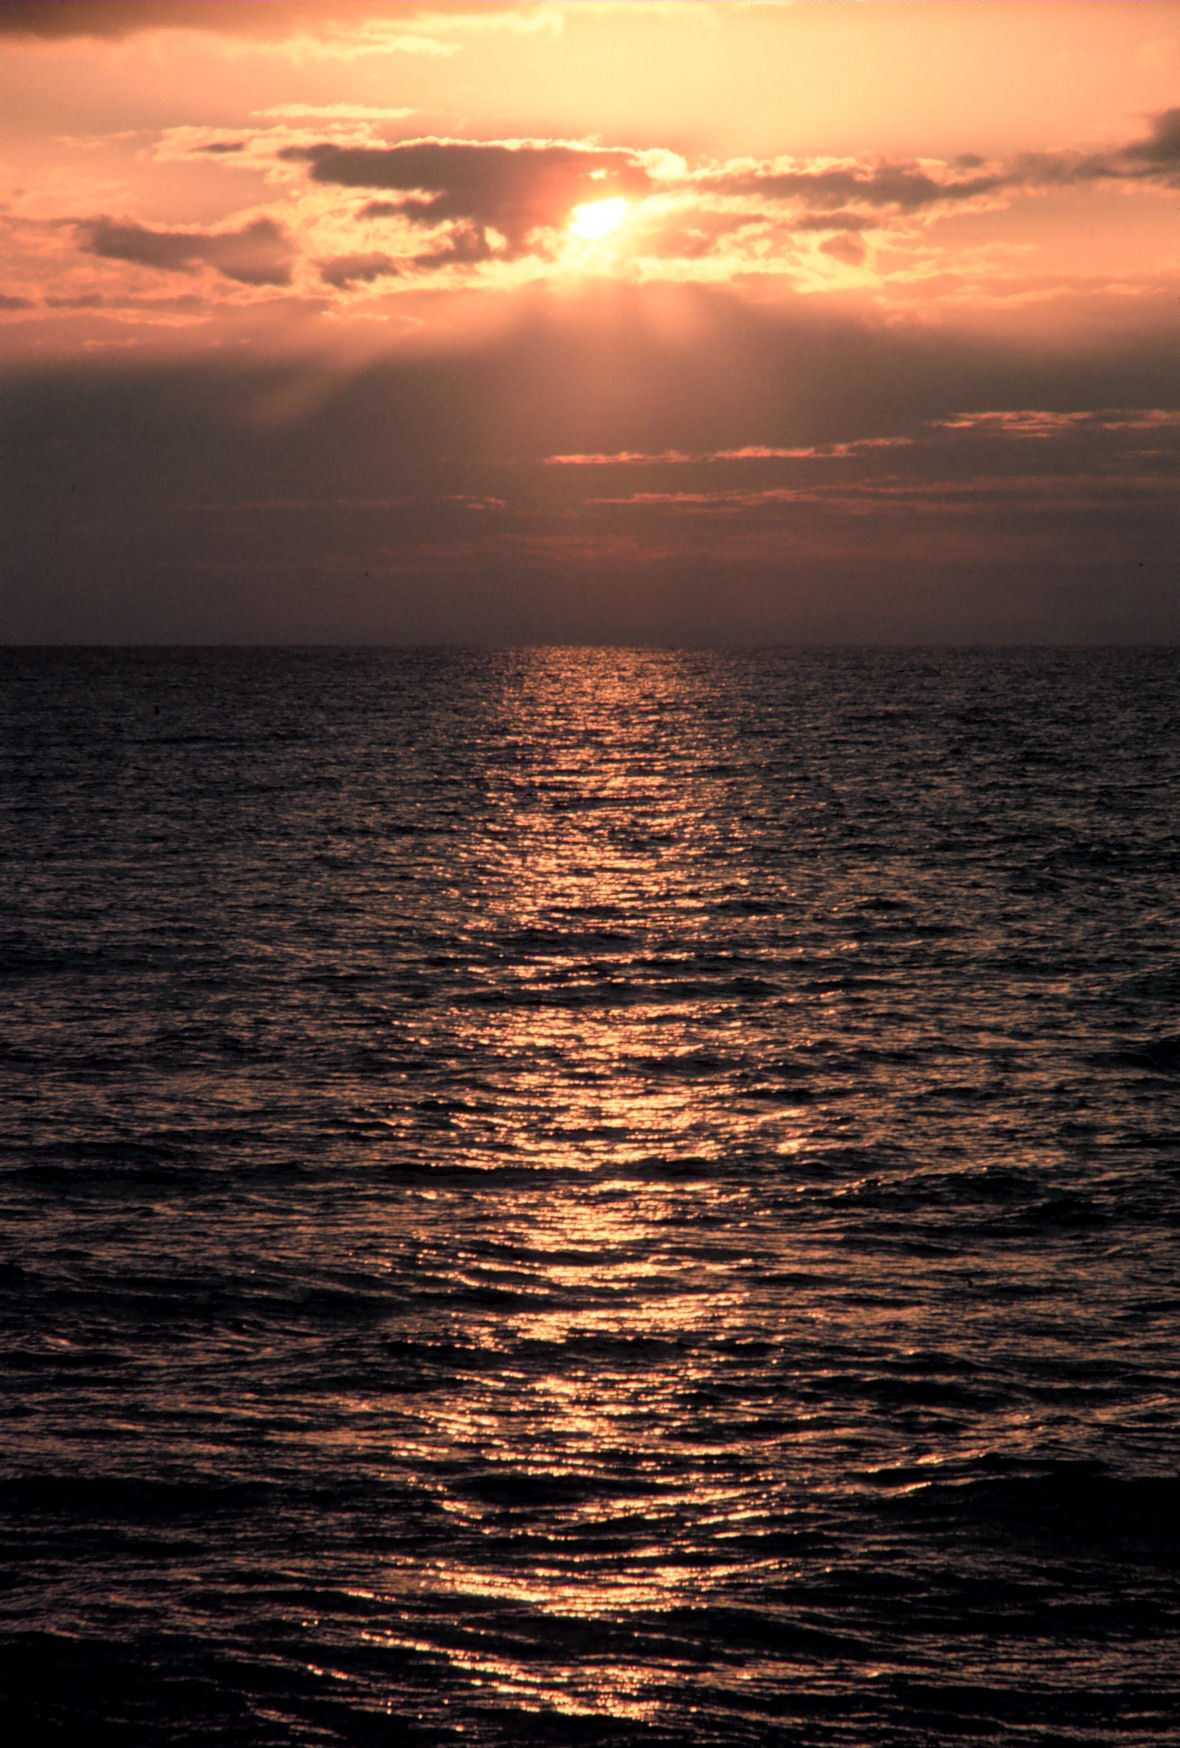
\includegraphics[scale=0.75]{figures/ocean300.jpg}
\caption{The late afternoon sun illuminating the ocean surface. Source: NOAA~\cite{misc:noaa}}
\end{figure}
%
\section{Problem Statement}
\label{sec:problem_statement}
%
Rendering an ocean is a demanding task for several reasons. First, consider the
sheer size of a water body as large as an ocean, which in numerous viewing
situations will be visible all the way to the horizon. Second, the ocean surface
is dynamic, therefore it needs to be constantly updated with the passage of time.
The wave interactions that give the ocean surface its shape are huge in terms of
complexity, thus we employ approximative models published by the oceanographic
research community.
Third, the optics of water are intricate. Incoming light may be reflected at the
surface or may be refracted into the water body, where the ratio between both is
dependent on the angle of incidence between the incoming light and the surface
normal at the point of incidence. Some of the refracted light may find its way
back to the ocean's surface, either by scattering inside the water body or by
reflection at the sea bottom, or possibly by a combination of both. Moreover,
waves on the ocean surface may break and cause surf and foam, both of which
interact with light drastically different than the surrounding water surface.
%
%  adding another
% layer of detail to the visual appearance of the ocean surface.
%
% The visual appearance of an ocean
% surface is highly dependent on its surroundings, because it reflects light from various
% sources e.g the sun, the skydome, clouds, as well as objects close to the
% water surface, such as boats and ships. Water does not only reflect light, it
% also refracts light, where the amount of refracted light to find its way back
% to the water surface is highly dependent on the depth of the water body.
% Moreover, the particulets contained inside the water body interact with the
% refracted light and therefore may cause a tint of the ocean surface.
% In addition, waves may break and cause surf and foam. Both interact with light
% drastically different than the surrounding water surface, adding another layer
% of detail.
%
%
%  (reflections), the depth of the underlying
% water body (refractions), as well as on the particulets contained in the water
% body itself (scattering).
% 
% The generation and animation of a water surface as large as an ocean is a demanding
% task. In most situations will often span all the way to the horizon, 
% 
% Some light is reflected, some is
% refracted, where the latter may or may not find its way back to the water
% surface.
%
\section{Scope and Focus of the Work}
\label{sec:scope_and_focus}
The scope of this thesis includes the generation, animation and rendering of the
surface of an open ocean in real-time. We focus our interest on the synthesis of
animated ocean surface geometry, for which we will adopt a set of mathematical
models from oceanographic research. Specific properties of said models allow for
easy addition and reduction of detail, as well as for a range of algorithmic
optimisations. The former combined with the latter gives us the opportunity to
strike a well-adjusted balance between model detail and computational workload,
and thereby to improve upon the status quo of current implementations.
%
% Note: The oceanographic models discussed in this work are not based on fluid
% dynamics, hence, convincing interaction between the ocean surface and other
% objects is beyond the scope of this thesis.
%
\section{Structure of the Work}
\label{sec:structure}
The remainder of this work is organized as follows: Chapter
\ref{ch:state_of_the_art} gives a survey of ocean simulation and rendering
methods. Chapter~\ref{ch:background} elaborates on the theoretical background
the oceanographic models are based on, as well as on the models themselves.
Chapter~\ref{ch:implementation} describes in detail the
synthesis of all data related to the ocean surface, including both the algorithmic
optimisations and the level of detail mechanism. Furthermore, we give an overview
of the rendering algorithms adopted for our implementation. In Chapter
\ref{ch:summary} we summarize our work and discuss the improvements we were able
to achieve in comparison to the state of the art. Moreover, we will suggest
future work based on open issues of our implementation.


%%%%%%%%%%%%%%%%%%%%%%%%%%%%%%%%%%%%%%%%%
%%%%%%%%%%%%%%%%%%%%%%%%%%%%%%%%%%%%%%%%%

%\chapter{Related Work}
\label{ch:state_of_the_art}
%
The ocean surface is an intricate phenomenon which owes its complexity
to its highly dynamic nature. Be it a quiet sea or an agitated one, small
turbulent waves or huge breaking ones, the underlying mechanisms are manifold
and act on a variety of scales. 
Surface tension, wind, earth's gravity, the gravitational pull of
sun and moon, all have an impact on ocean surface waves, where each force or
effect governs a different range of wavelengths.
Scientists have spent centuries trying to understand and explain these mechanisms.
%For example, ocean surface waves are in large
%part governed by the forces of wind and gravity, but capillary waves, often
%referred to as ripples, are dominated by surface tension, whereas tidal waves
%are caused by the gravitational pull of sun and moon. 
%with wavelengths less than a few centimeters and governed by surface tension, wind, storm, tsunami caused by earthquake, tidal waves
%
Oceanographic researchers define the behaviour of an ocean surface not based
on its influencing quantities, but based on its location. Water areas far from the
coast are called~\emph{deep water}, water areas close to shore are called
\emph{shallow water}, with \emph{intermediate} areas in between. Different
water locations are governed by different parameters. Deep ocean surfaces are
dominated by the interaction of wind and gravity at the interface
between air and water, whereas shallow water surfaces are characterized by waves
breaking near the shore. Deep water may ignore changes in water depth,
whereas intermediate and shallow waters need to account for how it affects
surface waves. Additionally, tidal waves and tsunamis may travel unnoticed
through deep water, but have a measurable impact on intermediate water areas
and even more so on shallow water areas.
% 
% The remainder of this chapter is organized as follows:
% Section~\ref{sec:simulation} gives an overview of simulation techniques used in
% computer graphics to synthesize various types of ocean surfaces.
% Section~\ref{sec:rendering} on the other hand discusses a compact set of 
% realtime ocean surface rendering algorithms.
%

To date, computer graphics employs several ocean wave simulation models which
may be roughly separated into three families: parametric description, spectral
description, and computational fluid dynamics (CFD). The first describes the water
surface by means of parametric equations which have been derived based on real
world observations \citep{Gerstner:1809,Rankine:1863,Biesel:1952}.
The second family approximate the ocean surface using wave spectra which
simulate the sea as a random process based on the distribution of wave energy
in frequency space \citep{book:kinsman2002wind}.
Third, computational fluid dynamics in combination with the Navier-Stokes
equations (NSE) are potentially able to fully describe the dynamics of all kinds of
fluid, including the ocean. We will omit any further discussion regarding CFD and NSE,
because, one, those models are the ones with the largest computational cost and therefore
the least adequate to simulate an entire ocean, and two,
the low degree of control over the simulation these algorithms allow for
may cause the user to be unable to get the desired results.
The interested reader may consult \cite{Bridson:2015} and \cite{egstar:2014} though.


% The next sections will give an overview of two families of simulation models,
% the one based on a parametric description of ocean waves and the one based
% on a spectral description. We will omit any discussion regarding CFD and NSE,
% because those models do not fit the the premise of this work.
% and the spectral description
% We will not discuss CFD and NSE any further, as
% they are out of scope for this work, for two reasons: first, too little user control
% over the simulation, second computational cost.
% The computational cost to simulate a water
% body as large as the ocean with CFD and NSE would exceed the realtime capabilities
% of CPUs and GPUs currently available to end users. FIXME: Short discussion of NSE and dismiss them, because
% out of scope. \cite{Bridson:2015} \cite{egstar:2014}
%
\section{Parametric Models}
%
\begin{figure}
\centering
 \subtop[]
 {
  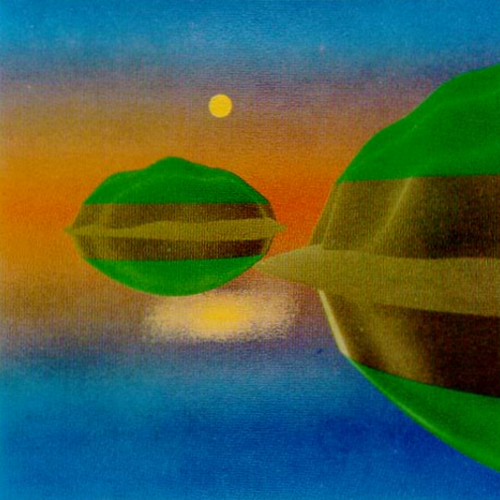
\includegraphics[scale=0.25]{figures/Vectorized_Procedural_Models_for_Natural_Terrain_-_Max_1981-006_1.png}
	\label{fig:max1981:1}
 }
 \hfill
 \subtop[]
 {
  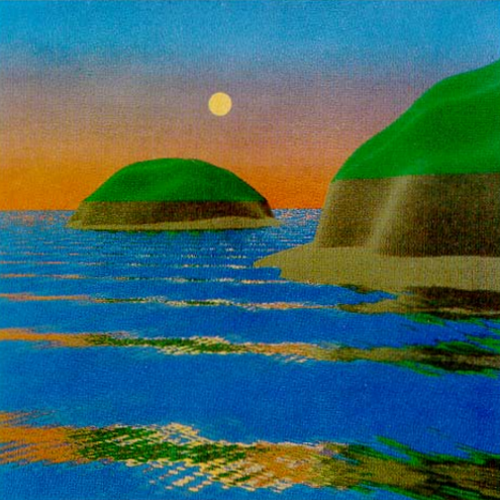
\includegraphics[scale=0.25]{figures/Vectorized_Procedural_Models_for_Natural_Terrain_-_Max_1981-007_1.png}
	\label{fig:max1981:2}
 }
 \hfill
 \subtop[]
 {
  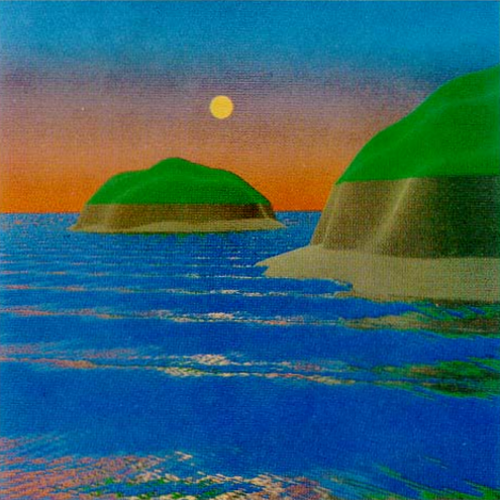
\includegraphics[scale=0.25]{figures/Vectorized_Procedural_Models_for_Natural_Terrain_-_Max_1981-006_2.png}
	\label{fig:max1981:3}
 }
 \hfill
 \subtop[]
 {
  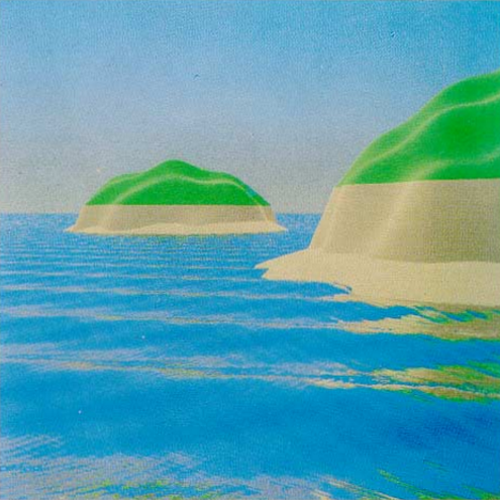
\includegraphics[scale=0.25]{figures/Vectorized_Procedural_Models_for_Natural_Terrain_-_Max_1981-007_2.png}
	\label{fig:max1981:4}
 }
\caption{\subcaptionref{fig:max1981:1}~Still water near sunset.
\subcaptionref{fig:max1981:2} One reflection from waves.
\subcaptionref{fig:max1981:3} Two reflections from waves.
\subcaptionref{fig:max1981:4} Early afternoon, two reflections from waves.
Source:~\cite{Max:1981}}
\label{fig:max1981}
\end{figure}
%
Parametric models are generally bound to the spatial domain, where they
generate and animate the ocean surface by means of a sum of periodical functions
which evolve throughout time using a phase difference. One of the earliest works
in this realm of computer graphics has been done by~\citet{Max:1981}. The ocean
surface is represented as a height map, where for each point $(x,z)$ at time $t$
the height is computed as a sum of sinusoids:
\begin{equation}
h(x,z,t) = y + \sum_{i=1}^N A_i \cos (l_i x + m_i z - \omega_i t)
\end{equation}
where $y$ is the mean height of the free surface, $N$ is the number of waves,
$A_i$ is the amplitude of the $i$th wave, $\mvec{k}_i = (l_i, m_i)$ its wave
vector, and $\omega_i$ its angular frequency. The wave vector defines the
travelling direction of the wave, with the the positive X-axis pointing towards
the coastline, the Y-axis pointing in the opposite direction of earth's gravity,
and the Z-axis aligned with the coastline. For the sum of waves to achieve a
realistic shape, \citeauthor{Max:1981} applies linear wave theory \citep{book:airy1845tides}:
the waves on the water surface are assumed to be dominated by gravity, the wave
amplitudes are assumed to be small in relation to the size of the water body,
and the water body is assumed to have infinite depth. Then, according to linear
wave theory it follows that the wave number $k=\norm{\mvec{k}}$ and the angular
frequency $\omega$ are related by $\omega^2=kg$, where $g=9.81$ denotes earth's
gravity. Results obtained by~\citeauthor{Max:1981} are shown in
Figure~\ref{fig:max1981}.
%
\begin{figure}
 \centering
 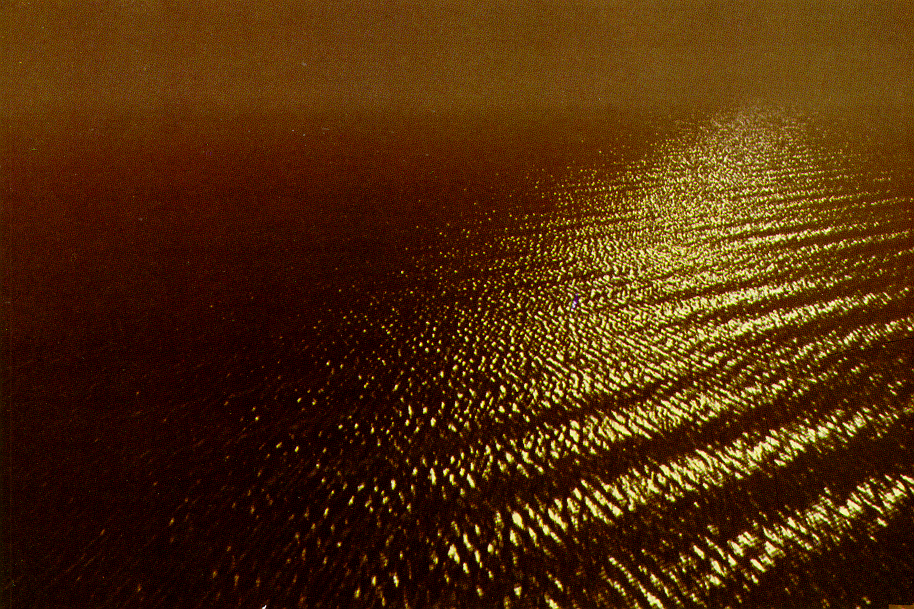
\includegraphics[scale=0.25]{figures/An_Image_Synthesizer_-_Perlin_1985-021.png}
 \caption{Ocean sunset. Source:~\cite{Perlin:1985}}
\label{fig:perlin1985}
\end{figure}
%
Both~\cite{Schachter:1980} and~\cite{Perlin:1985} developed similar approaches,
but instead of generating any actual geometry they simply distort the normal
vectors of given surfaces. Results obtained by~\citeauthor{Perlin:1985} are shown
in Figure~\ref{fig:perlin1985}.
%
\begin{figure}
 \centering
 \subtop[]
 {
  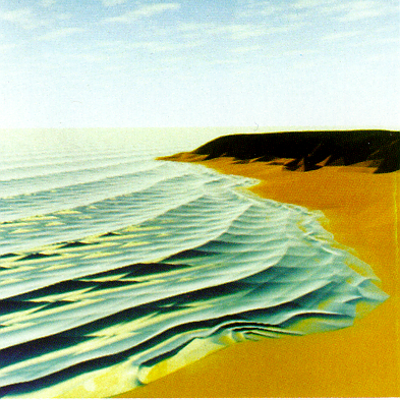
\includegraphics[scale=0.25]{figures/Modeling_Waves_and_Surf_-_Peachey_1986-009.png}
	\label{fig:peachey1986:1}
 }
 \hfill
 \subtop[]
 {
  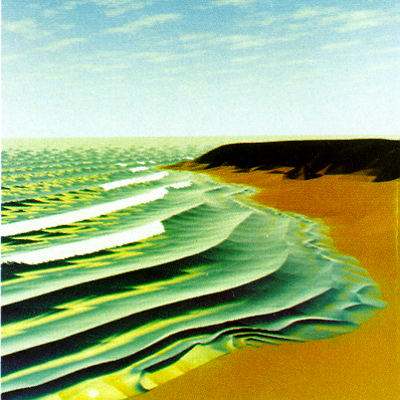
\includegraphics[scale=0.25]{figures/Modeling_Waves_and_Surf_-_Peachey_1986-010.png}
	\label{fig:peachey1986:2}
 }
 \hfill
 \subtop[]
 {
  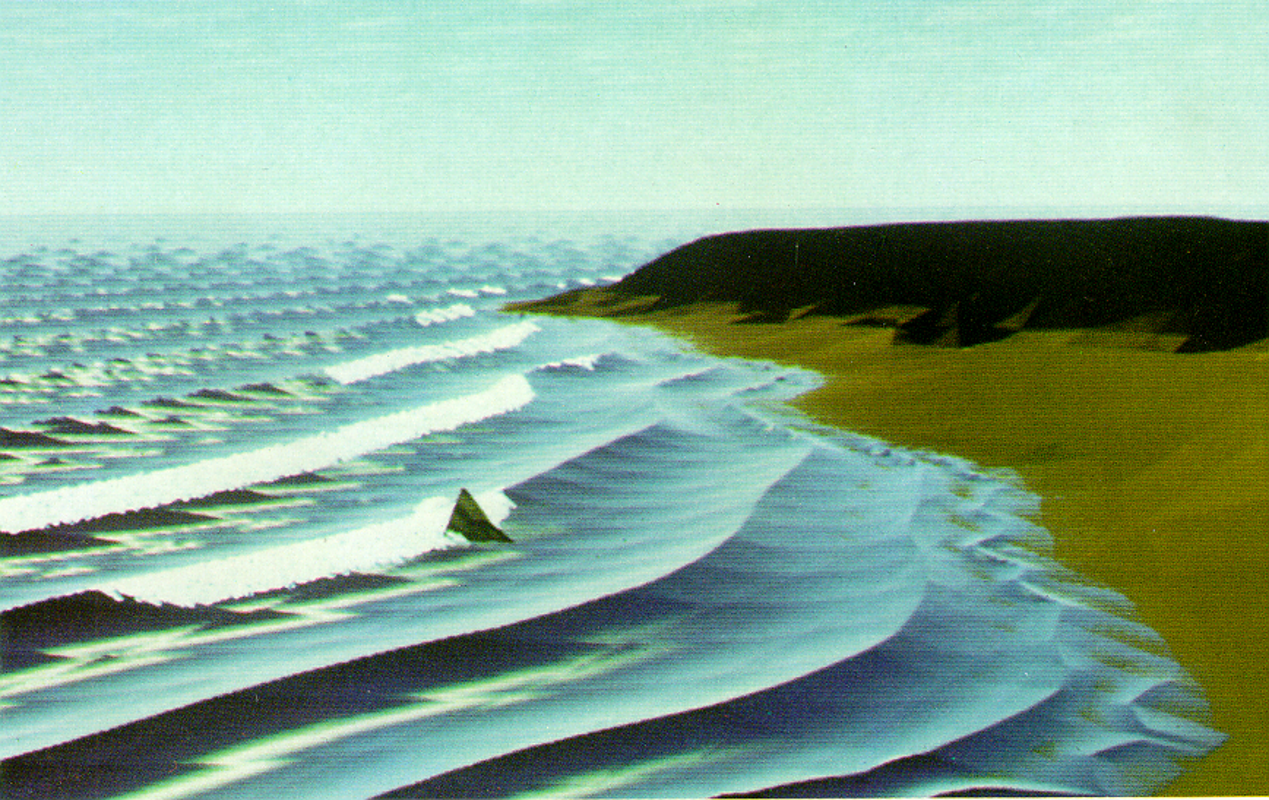
\includegraphics[scale=0.125]{figures/Modeling_Waves_and_Surf_-_Peachey_1986-012.png}
	\label{fig:peachey1986:3}
 }
 \caption{\subcaptionref{fig:peachey1986:1}~Waves on the beach.
\subcaptionref{fig:peachey1986:2}~Breaking waves on the beach.
\subcaptionref{fig:peachey1986:3}~Breaking waves with obstacle.
Source:~\cite{Peachey:1986}}
\label{fig:peachey1986}
\end{figure}
%

The assumption of infinite depth restricts the above methods to deep water, they
are unable to include phenomena which arise near the shore, such as breaking
waves and wave refraction. \cite{Peachey:1986}, still in the realm of linear
wave theory, simulates waves near the shore through the relationship
$\omega^2=kg\tanh (kh)$, where $h$ is the water depth. Moreover,
\citeauthor{Peachey:1986} does not only distort waves approaching the sloping beach
so that they resemble breaking waves more closely, but also adds particle systems
to generate spray. Results of \cite{Peachey:1986} are shown in Figure~\ref{fig:peachey1986}.
%
\begin{figure}
\begin{tikzpicture}
\begin{axis}[
	width=\textwidth,
	height=0.5\textwidth,
	domain=0:40,
	%xmin = 0,
	%xmax = 40,
	%axis equal,
	xtick=\empty,
	%ytick=\empty,
	%y tick label style={anchor=west,xshift=\pgfkeysvalueof{/pgfplots/major tick length}},
	yticklabels={$kA=0.2$,$kA=0.7$,$kA=1.0$,$kA=1.3$},
	ytick={12,8,4,0} 
	]
\addplot[samples=300,domain=0:40] ({x+0.2*sin(deg(1*x-sqrt(9.81*1)*0))}, {12-0.2*cos(deg(1*x-sqrt(9.81*1)*0))});
\addplot[samples=300,domain=0:40] ({x+0.7*sin(deg(1*x-sqrt(9.81*1)*0))}, { 8-0.7*cos(deg(1*x-sqrt(9.81*1)*0))});
\addplot[samples=300,domain=0:40] ({x+1.0*sin(deg(1*x-sqrt(9.81*1)*0))}, { 4-1.0*cos(deg(1*x-sqrt(9.81*1)*0))});
\addplot[samples=300,domain=0:40] ({x+1.3*sin(deg(1*x-sqrt(9.81*1)*0))}, { 0-1.3*cos(deg(1*x-sqrt(9.81*1)*0))});
\end{axis}
\end{tikzpicture}
\caption{Example waves with different $kA$. One can see that the wave crest gets more pronounced as $kA$ grows,
with the wave intersecting itself when $kA > 1$.}
\label{fig:trochoid:crests}
\end{figure}
%

\cite{Fournier:1986}, instead of using sinusoids, build on Gerstner's work
\citep{Gerstner:1809, Rankine:1863} to synthesize waves. Gerstner waves assume
a water surface dominated by gravity and an incompressible water body of
infinite depth. A single wave may be written as follows:
\begin{align}
\mvec{x} &= \mvec{x}_0 - \frac{\mvec{k}}{\norm{\mvec{k}}} A \sin\left(\mvec{k}\cdot\mvec{x}_0-\omega t\right)\\
y &= y_0 - A \cos\left(\mvec{k}\cdot\mvec{x}_0-\omega t\right)
\end{align}
where $\mvec{x}$ denotes the horizontal coordinate and $y$ the vertical coordinate
of the wave particle at time $t$, with $\mvec{x}_0$ and $y_0$ its horizontal
and vertical position at rest respectively. As before, $A$ is the amplitude,
$\mvec{k}$ the wave vector and $\omega$ the wave's angular frequency. Given the
wave number $k=\norm{\mvec{k}}$, the term $kA$ defines the sharpness of the wave
crest. With $kA<1$ the wave takes the form of an upside-down trochoid, with
$kA=1$ the form of an upside-down cycloid, and with $kA>1$ the wave intersects
itself, an undesireable effect which does not resemble real waves.
See Figure~\ref{fig:trochoid:crests} for waves with different $kA$.
%Gerstner waves take the form of an upside-down trochoid.
The sum of of Gerstner waves is as follows:
\begin{align}
\mvec{x} &= \mvec{x}_0 - \sum_i^N\frac{\mvec{k}_i}{\norm{\mvec{k_i}}} A_i \sin\left(\mvec{k}_i\cdot\mvec{x}_0-\omega t\right)\\
y &= y_0 - \sum_i^N A_i \cos\left(\mvec{k}_i\cdot\mvec{x}_0-\omega t\right)
\end{align}
%
%
\begin{figure}
 \centering
 \subtop[]
 {
  
\includegraphics[scale=0.175]{figures/A_Simple_Model_of_Ocean_Waves_-_Fournier_1986-004_1.png}
	\label{fig:fournier1986:refraction:1}
 }
 \hfill
 \subtop[]
 {
  
\includegraphics[scale=0.175]{figures/A_Simple_Model_of_Ocean_Waves_-_Fournier_1986-004_2.png}
	\label{fig:fournier1986:refraction:2}
 }
 \hfill
 \subtop[]
 {
  
\includegraphics[scale=0.175]{figures/A_Simple_Model_of_Ocean_Waves_-_Fournier_1986-005_1.png}
	\label{fig:fournier1986:refraction:3}
 }
 \caption{The refraction of waves.
\subcaptionref{fig:fournier1986:refraction:1} Two bottoms of constant depth, the
wavelengths are halved as the waves reach the shallow bottom on the left.
\subcaptionref{fig:fournier1986:refraction:2} The beach slopes gently down from
the left. One can see the wave fronts aligning themselves with the beach.
\subcaptionref{fig:fournier1986:refraction:3} An undersea valley that affects
both, the wavelengths as well as the travelling direction of the waves.
Source:~\cite{Fournier:1986}}
\label{fig:fournier1986:refraction}
\end{figure}
%
\begin{figure}
 \centering
 \subtop[]
 {
  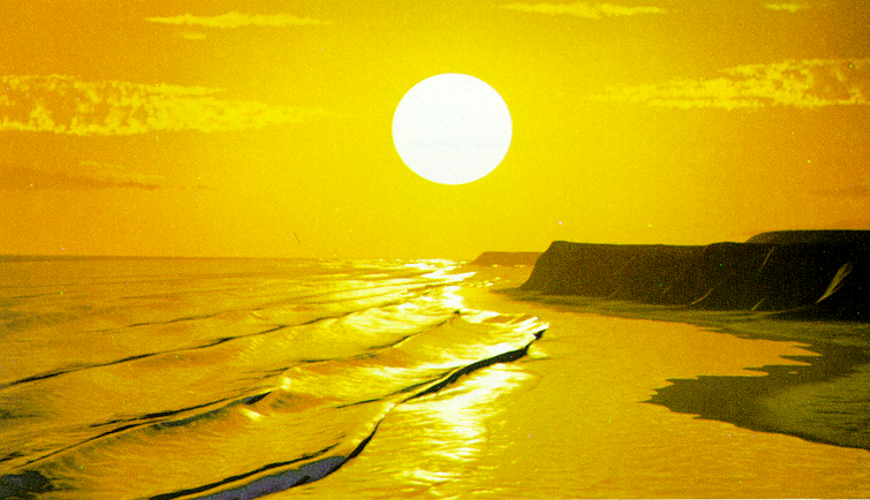
\includegraphics[scale=0.225]{figures/A_Simple_Model_of_Ocean_Waves_-_Fournier_1986-008.png}
	\label{fig:fournier1986:results:1}
 }
 \hfill
 \subtop[]
 {
  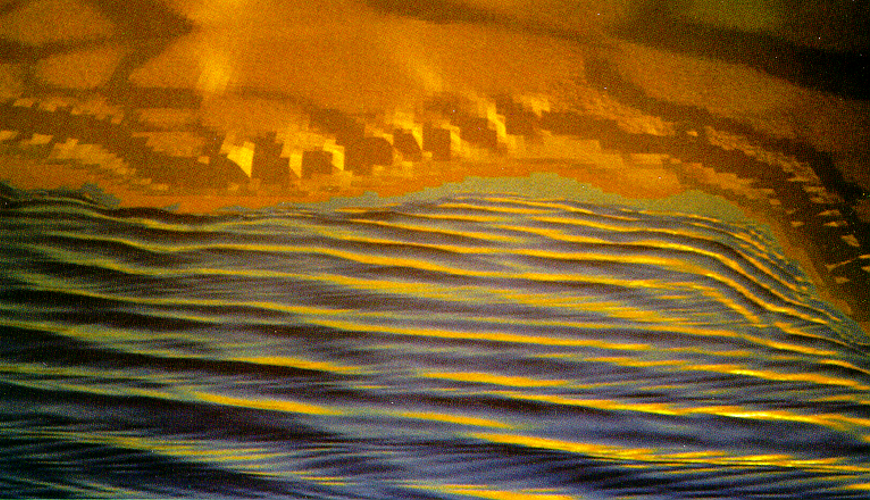
\includegraphics[scale=0.225]{figures/A_Simple_Model_of_Ocean_Waves_-_Fournier_1986-010.png}
	\label{fig:fournier1986:results:2}
 }
 \subtop[]
 {
  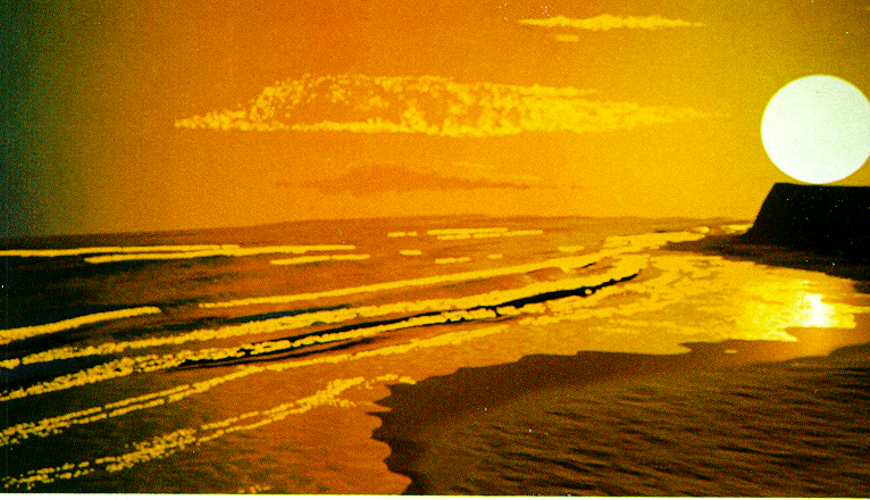
\includegraphics[scale=0.225]{figures/A_Simple_Model_of_Ocean_Waves_-_Fournier_1986-011.png}
	\label{fig:fournier1986:results:3}
 }
 \hfill
 \subtop[]
 {
  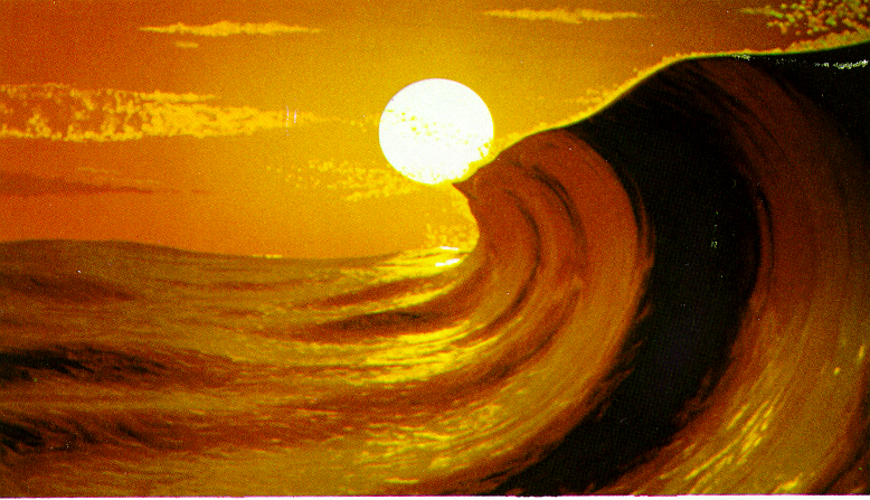
\includegraphics[scale=0.225]{figures/A_Simple_Model_of_Ocean_Waves_-_Fournier_1986-013.png}
	\label{fig:fournier1986:results:4}
 }
 \caption{
 \subcaptionref{fig:fournier1986:results:1} Breaking waves on the shore, where the crests take the shape of the shore.
 \subcaptionref{fig:fournier1986:results:2} Wave refraction.
 \subcaptionref{fig:fournier1986:results:3} Waves with spray and foam.
 \subcaptionref{fig:fournier1986:results:4} A large breaking wave.
 Source:~\cite{Fournier:1986}
 }
 \label{fig:fournier1986:results}
\end{figure}
%
\citeauthor{Fournier:1986} improve upon the above model in two ways. First, wave
particle motion takes the underlying sea bed into account, allowing for waves
to be refracted i.e. to change their wavelength, their speed and their direction
of travel based on water depth, see Figure~\ref{fig:fournier1986:refraction}.
Second, the circular orbit of Gerstner waves approaching the shore is
transformed into an elliptical orbit, which allows to approximate the form of
breaking waves near the beach. Results of \cite{Fournier:1986} are shown in
Figure~\ref{fig:fournier1986:results}.
%
\begin{figure}
 \centering
 \subtop[]
 {
  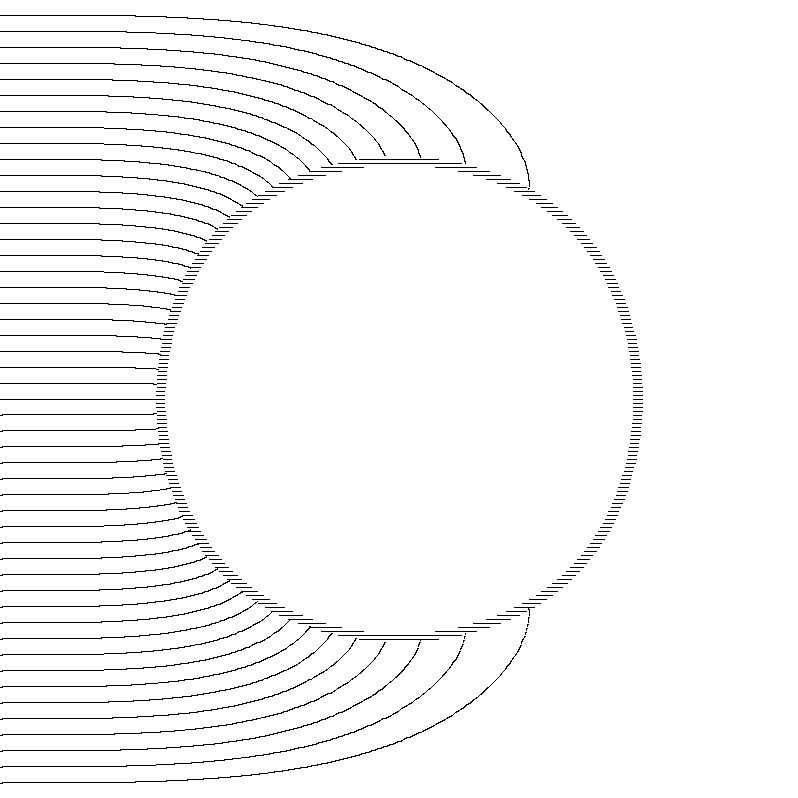
\includegraphics[width=0.2\textwidth]{figures/A_phenomenological_model_of_coastal_scenes_based_on_physical_considerations_-_Gonzato_1997-051.png}
	\label{fig:gonzato1997:results:1}
 }
 \hfill
 \subtop[]
 {
  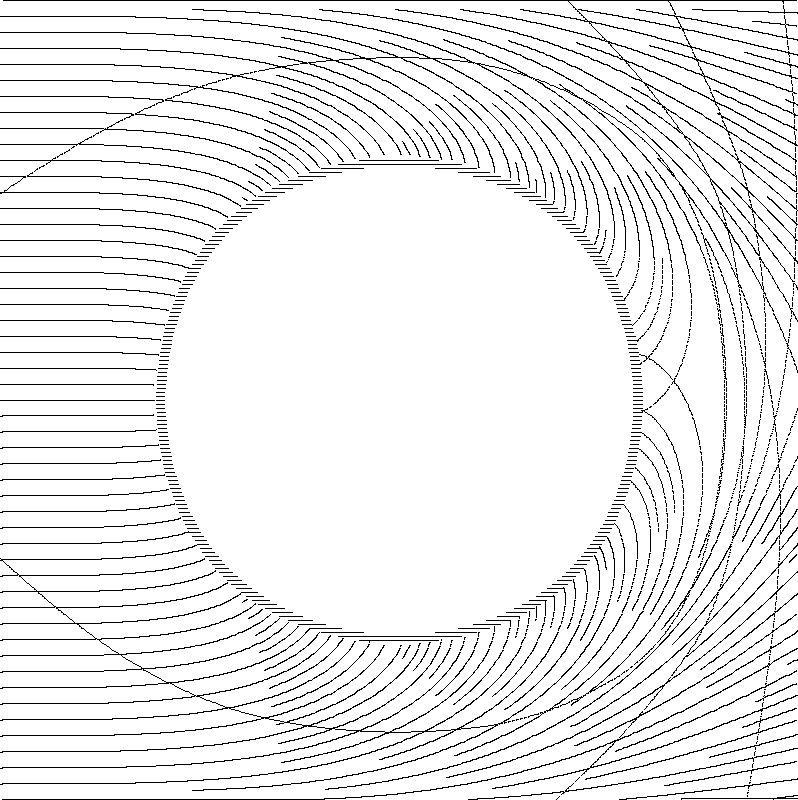
\includegraphics[width=0.2\textwidth]{figures/A_phenomenological_model_of_coastal_scenes_based_on_physical_considerations_-_Gonzato_1997-055.png}
	\label{fig:gonzato1997:results:2}
 }
 \hfill
 \subtop[]
 {
  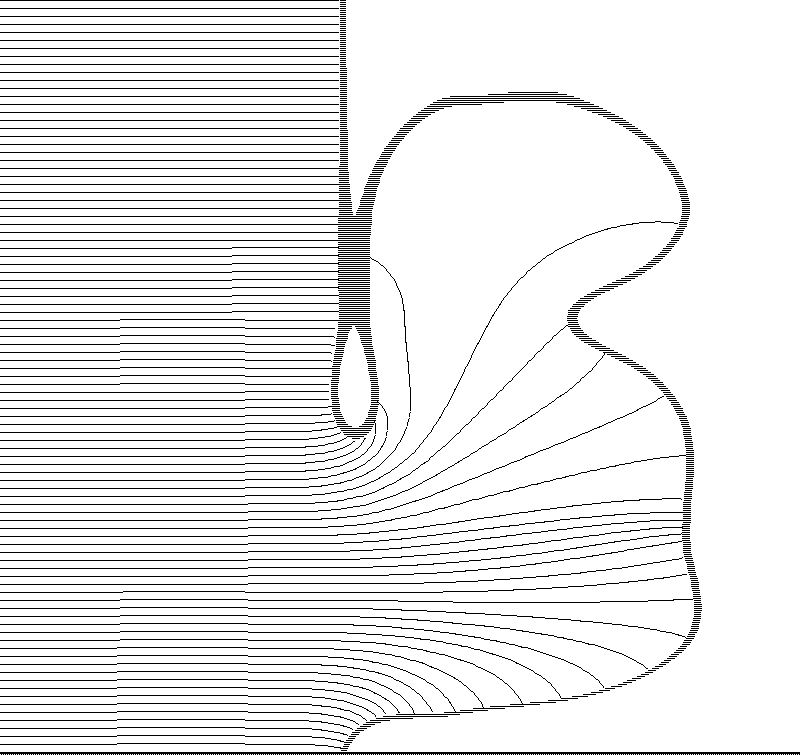
\includegraphics[width=0.2\textwidth]{figures/A_phenomenological_model_of_coastal_scenes_based_on_physical_considerations_-_Gonzato_1997-052.png}
	\label{fig:gonzato1997:results:3}
 }
 \hfill
 \subtop[]
 {
  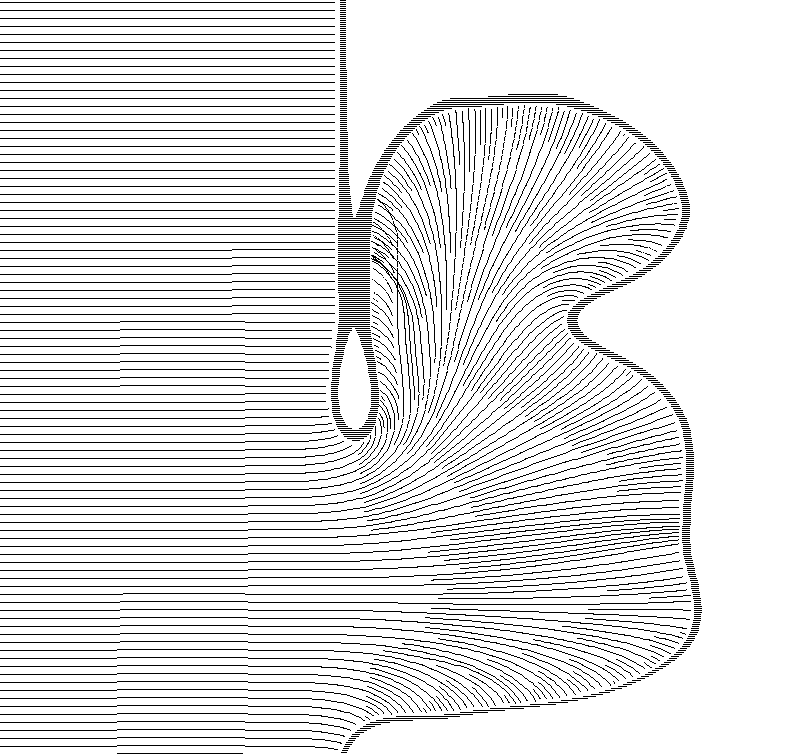
\includegraphics[width=0.2\textwidth]{figures/A_phenomenological_model_of_coastal_scenes_based_on_physical_considerations_-_Gonzato_1997-056.png}
	\label{fig:gonzato1997:results:4}
 }
 \caption{
 \subcaptionref{fig:gonzato1997:results:1} Wave Trace of an island.
 \subcaptionref{fig:gonzato1997:results:2} Dynamic Wave Trace of the same island.
 \subcaptionref{fig:gonzato1997:results:3} Wave Trace of a bay.
 \subcaptionref{fig:gonzato1997:results:4} Dynamic Wave Trace of the same bay.
 Source:~\cite{Gonzato:1997}
 }
 \label{fig:gonzato1997:results}
\end{figure}
%
\cite{Ts'o:1987} implement an algorithm called \emph{wave tracing} which
launches orthogonal wave rays from the open sea along the direction of wave
propagation. Wave refraction is computed based on Snell's law, the wave trains
are traced inside a uniform grid. In case rays tracing the waves path diverge
significantly from a straight line, there may remain undersampled areas,
leading to parts of the surface lacking detail. \cite{Gonzato:1997} improve
upon this by generating new rays in undersampled areas, allowing their
\emph{dynamic wave tracing} algorithm to more densely sample the water surface
surrounding islands and the water surface inside bays. See Figure
\ref{fig:gonzato1997:results} for a comparison between wave tracing and
dynamic wave tracing. Moreover,
\citeauthor{Gonzato:1997} modify the wave model to include plunging breaking
waves. Three additional functions achieve said goal.
First, a stretch function which imitates Biesel law~\citep{Biesel:1952} by
progressively stretching the wave on the crest along its major axis. Second and
third, an orientation and a displacement function to rotate the wave's crest
downwards, towards the water surface below the crest. Later,
\citeauthor{Gonzato:2000} extend their work to include wave diffraction, see
\cite{Gonzato:2000}.\\

Parametric models are well suited to model propagating water fronts, where a
small number of wave numbers may suffice to obtain satisfactory results. 
Because one has basically to select the involved wave lengths and amplitudes
by trial and error, it follows that parametric models are not particularly
eligible to represent an agitated water surface, as it would involve a
significant higher number of waves. The user may have a hard time assembling a
meaningful number of wave numbers and amplitudes, with the result being
potentially infeasible because of the accumulated computational cost.
%
%
\section{Spectral Models}
Oceanographic research employs~\emph{wave spectra} to model the deep ocean. The
sea is assumed as a linear superposition of sinusoids with many different wave
lengths, frequencies and phases, travelling in different directions. The wave
spectrum gives the distribution of wave energy among different wave frequencies
or wave lengths. Given horizontal coordinate $\mvec{x}$, we may compute the
vertical coordinate via an inverse Discrete Fourier Transform as follows:
\begin{equation}
h(\mvec{x},t) = \sum_{\mvec{k}}A(\mvec{k},t)\mathrm{e}^{\mathrm{i}\transpose{\mvec{k}}\mvec{x}}
\label{eq:spectral_models}
\end{equation}
where $\mvec{k}$ represent the wave vectors of the most significant frequency
components, and $A(\mvec{k},t)$ are the amplitudes obtained from the wave
spectrum. At this point we refer to Sections \ref{sec:linear_theory_ocean_waves}
and \ref{sec:random_sea} for a more thorough discussion of the theoretical
background of wave spectra, whereas Section \ref{sec:random_sea_discretisation}
explains Equation~\ref{eq:spectral_models} in detail. For now it shall suffice
to give an overview of key properties of wave spectra. 

First, all wave spectra
are static. Static in the sense, that a wave spectrum represents a certain sea
state based on parameters such as wind speed and the distance from shore. To
change the sea state requires the synthesis of a new wave spectrum. Thus, for
example, if one would like to simulate a calm sea which gets agitated as a storm
approaches, then one needs to generate different wave spectra and interpolate
between them.

Second, wave spectra are compact models which require only a small
number of input parameters defining the desired sea state. Since wave spectra
are homogeneous models, all parameters are uniform for the entire ocean surface,
there is no room for local variations as parametric models would allow. Wave
spectra assume the ocean surface to be dominated by the interplay of wind and
gravity, hence wind speed is the parameter common to all models. Another well
established parameter is~\emph{fetch}, which is the distance over which the wind
blows before it reaches the ocean patch the wave spectrum simulates. Water
depth, if supported by the wave spectrum model, like all other parameters is
uniform, hence the sea bed is assumed planar and parallel to the ocean surface
at rest. It follows that no wave transitions from one water depth to another,
therefore no wave refraction may take place.

Third, the inverse Discrete Fourier Transform may leverage the
Fast Fourier Transform algorithm~\citep{Cooley:1965}, which makes the computation of
Equation~\ref{eq:spectral_models} most efficient. Hence, given the same
computational cost, it is possible for spectral models to involve way more wave
numbers in the sum of waves than parametric models could. Moreover, thanks to
the Discrete Fourier Transform we get a seamless tileable surface.
The downside of the Fourier Transform is that the range and uniform sampling
density of spatial coordinates $\mvec{x}$ directly defines the set of wave
vectors $\mvec{k}$ contributing to the sum of waves. In contrast to the
parametric models we are neither able to cherry-pick certain wave vectors,
nor to omit a range of wave vectors, nor to to exert some form of local control
where we modify the set of wave vectors based on location $\mvec{x}$.\\

%
\begin{figure}
 \centering
 \subtop[]
 {
  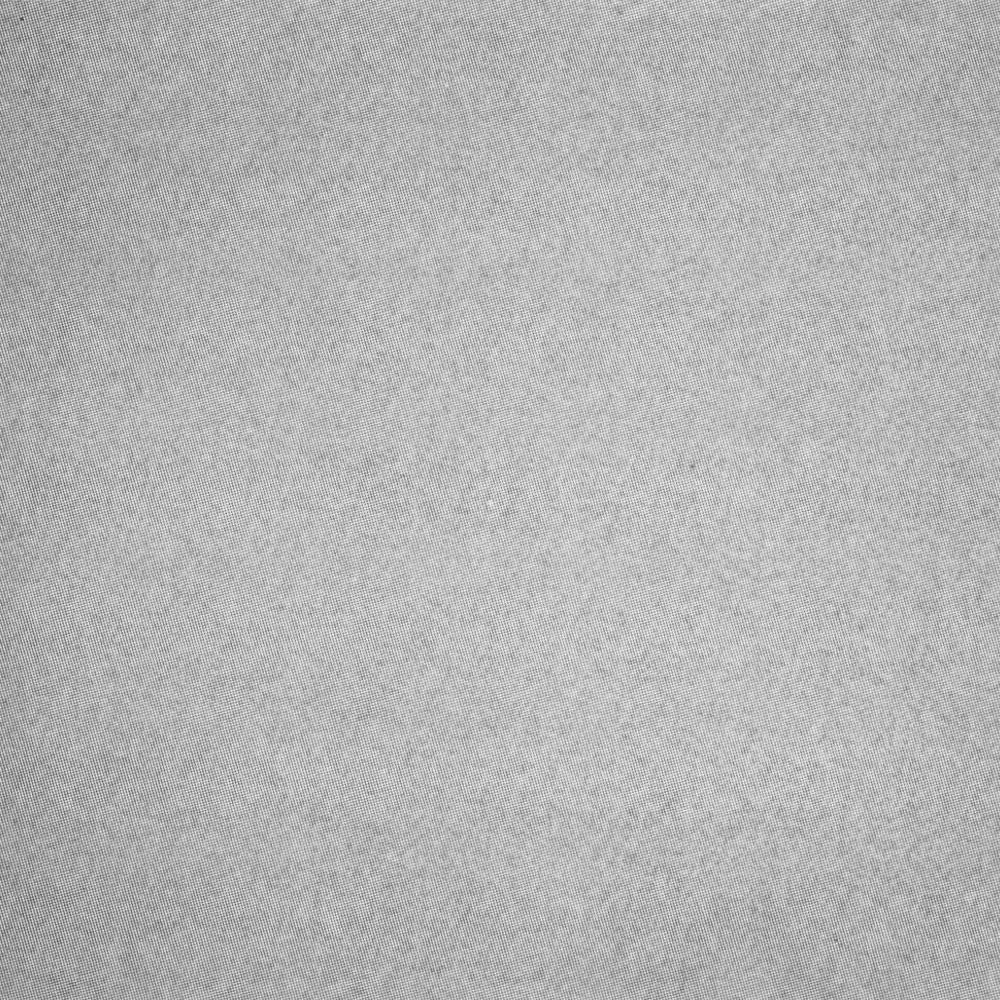
\includegraphics[scale=0.1125]{figures/Fourier_Synthesis_of_Ocean_Scenes_-_Mastin_1987-005_1.png}
	\label{fig:mastin_waves:1}
 }
 \hfill
 \subtop[]
 {
  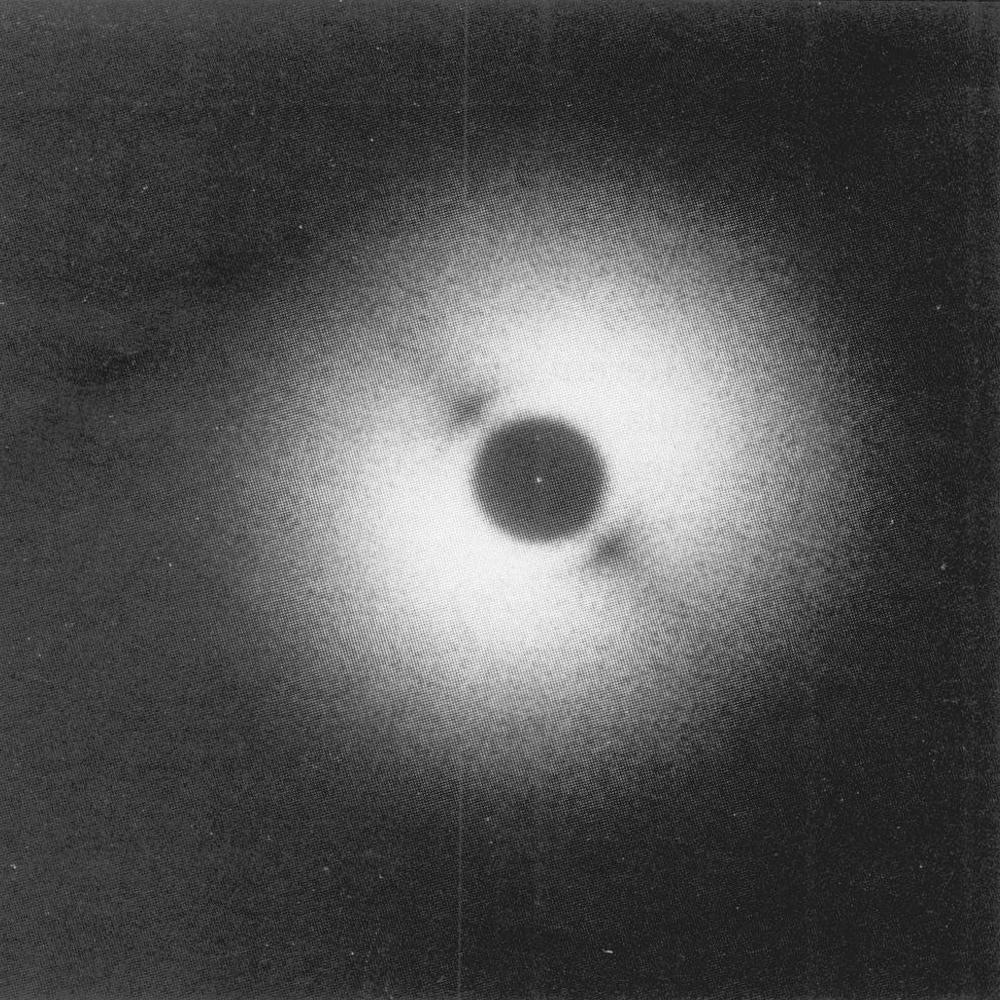
\includegraphics[scale=0.1125]{figures/Fourier_Synthesis_of_Ocean_Scenes_-_Mastin_1987-005_2.png}
	\label{fig:mastin_waves:2}
 }
 \hfill
 \subtop[]
 {
  
\includegraphics[scale=0.1125]{figures/Fourier_Synthesis_of_Ocean_Scenes_-_Mastin_1987-005_3.png}
	\label{fig:mastin_waves:3}
 }
 \hfill
 \subtop[]
 {
  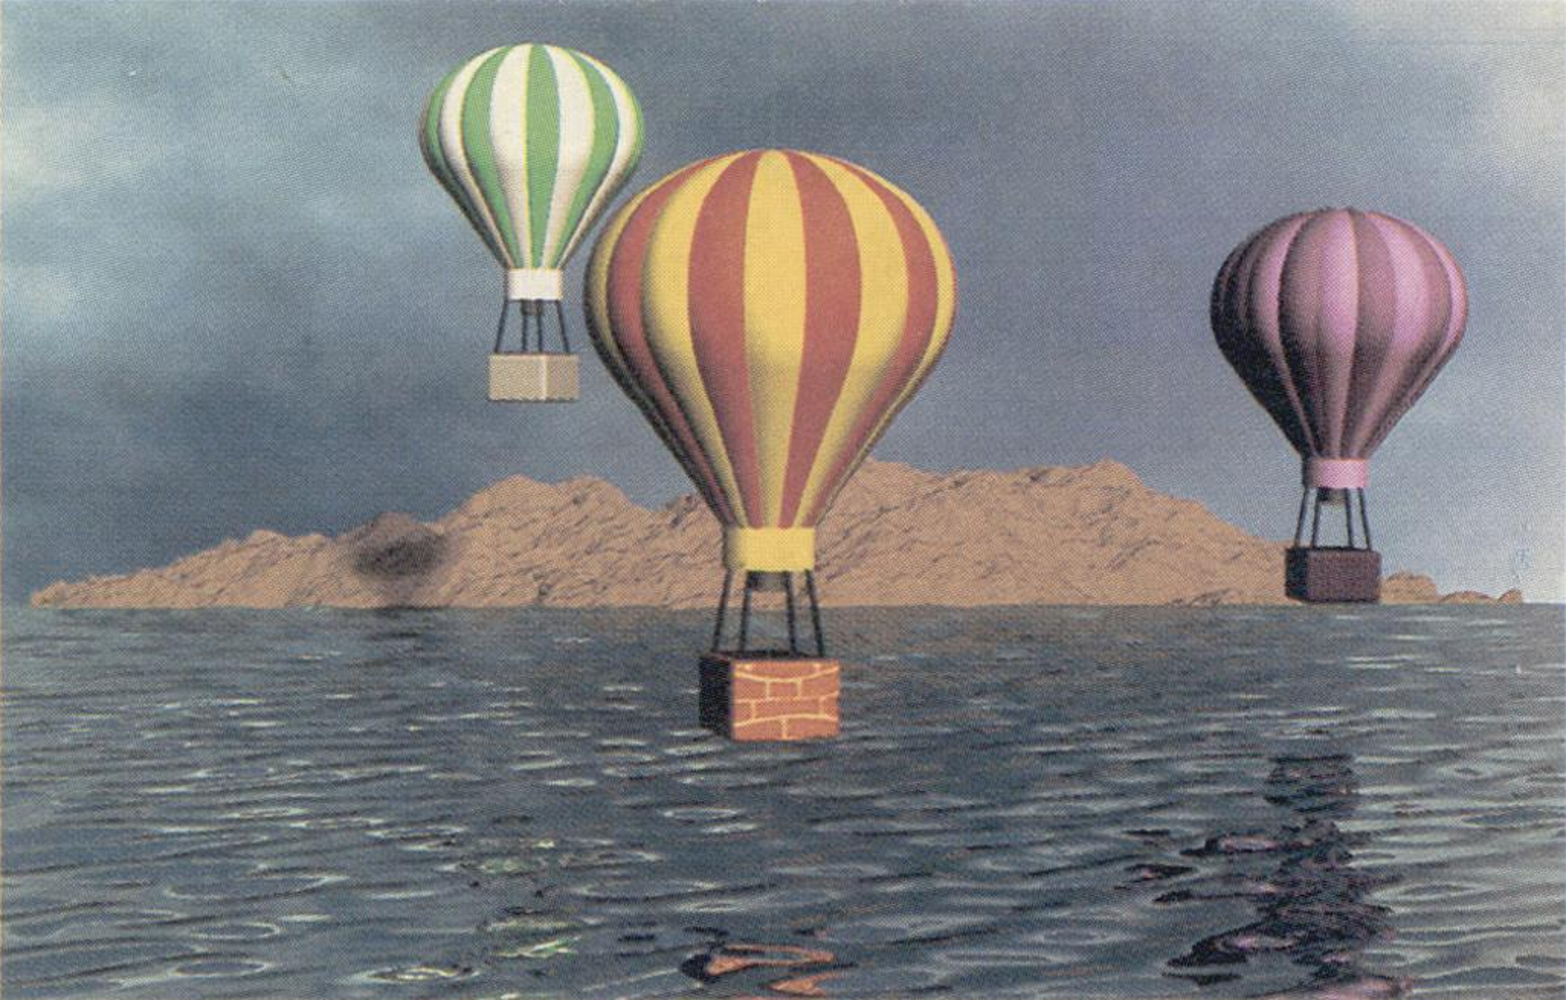
\includegraphics[scale=0.1125]{figures/Fourier_Synthesis_of_Ocean_Scenes_-_Mastin_1987-007_1.png}
	\label{fig:mastin_waves:4}
 }
 \caption{
\subcaptionref{fig:mastin_waves:1} White noise.
\subcaptionref{fig:mastin_waves:2} The Pierson-Moskowitz spectrum combined with the directional spreading function.
\subcaptionref{fig:mastin_waves:3} The synthesized heightfield.
\subcaptionref{fig:mastin_waves:4} Rendering of the sea surface.
Source: \cite{Mastin:1987}
}
\label{fig:mastin_waves}
\end{figure}
%
\cite{Mastin:1987} introduced wave spectra to computer graphics. Their approach
is a simple one: generate white noise to represent random amplitudes and phases,
then filter it with the Pierson-Moskowitz spectrum
\citep{article:PiersonMoskowitz1964} in frequency space. The Pierson-Moskowitz
spectrum gives wave energy per wave number, but not its distribution across
wave vectors. In short, there is no information telling in which direction the
waves are moving. Thus, \citeauthor{Mastin:1987} combine the Pierson-Moskowitz
spectrum with a \emph{directional spreading function}, namely the one proposed
in \cite{article:Hasselmann1980}. A directional
spreading function distributes wave energy across wave vectors, where
the energy peak is usually to be found aligned with the wind direction and the
remaining energy fanning out at its sides. Results of \cite{Mastin:1987} are
shown in Figure~\ref{fig:mastin_waves}.
\cite{Premoze:2000} on the other hand make use of the JONSWAP spectrum
\citep{article:Hasselman1973}, as it allows for more varied ocean surfaces than
the Pierson-Moskowitz spectrum.
An in-depth discussion of the Pierson-Moskowitz spectrum, the JONSWAP spectrum,
as well as directional spreading functions is to be found in Section
\ref{sec:1d_frequency_spectra}.

%
\begin{figure}
 \centering
 \subtop[]
 {
  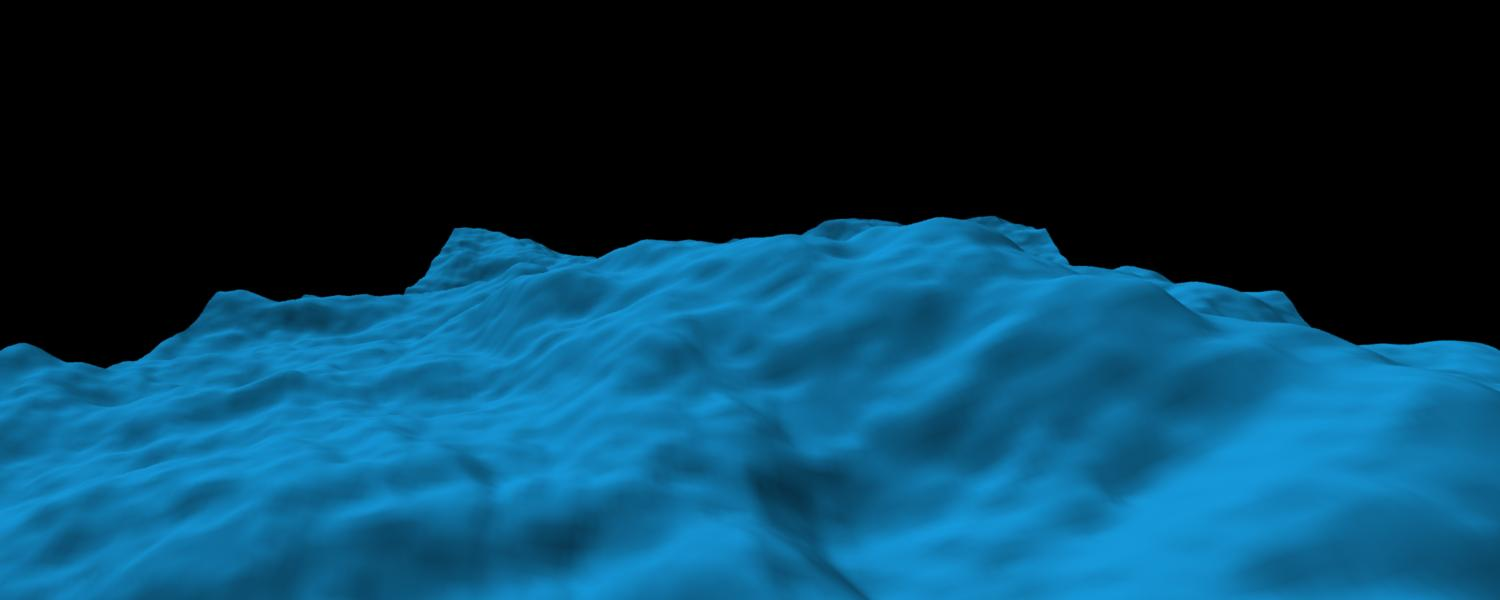
\includegraphics[scale=0.125]{figures/Simulating_Ocean_Water-012.png}
	\label{fig:tessendorf_choppy_waves:1}
 }
 \hfill
 \subtop[]
 {
  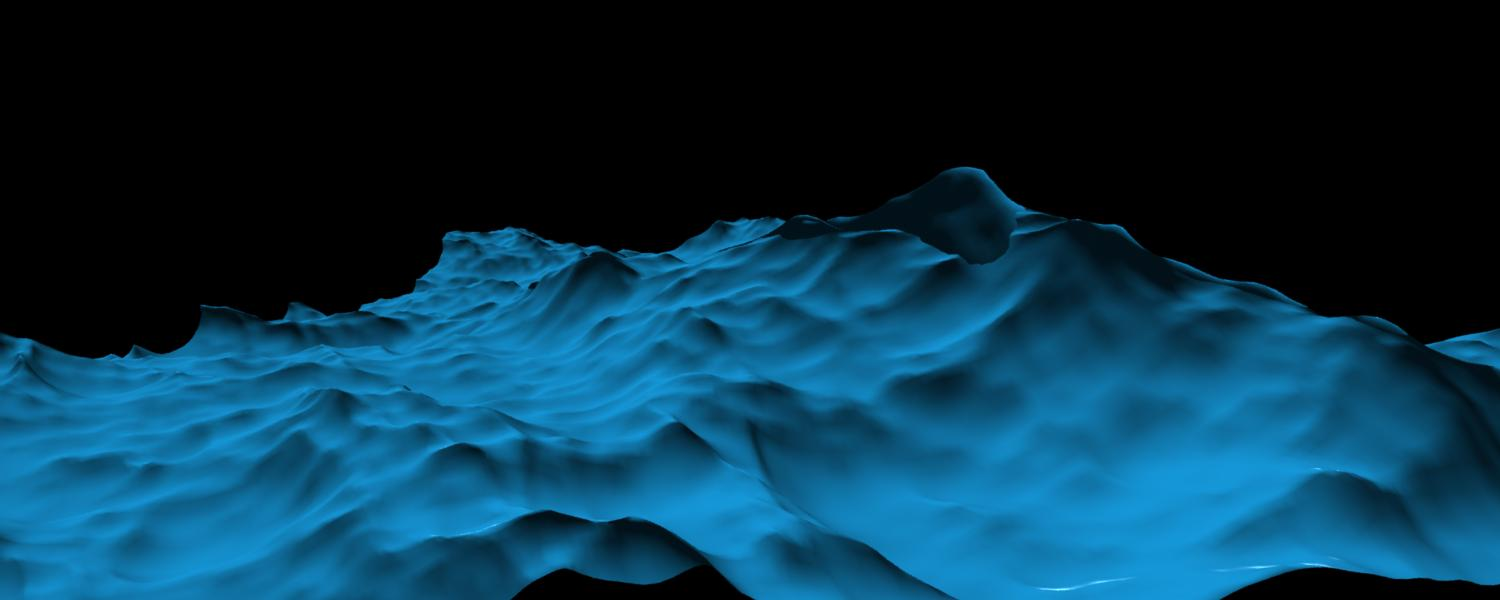
\includegraphics[scale=0.125]{figures/Simulating_Ocean_Water-013.png}
	\label{fig:tessendorf_choppy_waves:2}
 }
 \caption{
\subcaptionref{fig:tessendorf_choppy_waves:1} Ocean surface sythesized with the Phillips spectrum.
\subcaptionref{fig:tessendorf_choppy_waves:2} The same surface with the choppy wave algorithm applied.
Source: \cite{course:simulatingocean}
}
\label{fig:tessendorf_choppy_waves}
\end{figure}
%
One of the most known works in computer graphics related to wave spectra is
\cite{course:simulatingocean}. Therein, \citeauthor{course:simulatingocean}
describes how the ocean was brought to life for productions such as
\emph{Waterworld} and \emph{Titanic}. In contrast to \citeauthor{Mastin:1987},
\citeauthor{course:simulatingocean} does not use white noise, but Gaussian
random numbers, because waves in deep sea areas are often observed to follow a
Gaussian distribution. Moreover, \citeauthor{course:simulatingocean}
makes use of the Phillips spectrum, a spectrum not found in oceanographic
research, but devised by himself specifically for computer graphics purposes.
%\cite{article:Phillips1958,article:Phillips1985}
Ocean surfaces based on wave spectra all share the same issue, namely the all to
gentle form of wave troughs and wave crests. Because the surface is computed as
a linear superposition of sinusoids, it is only natural that the result shares
the general form of its underlying building blocks. But a sea exposed to strong
winds or even a storm is characterized by steep waves with sharp crests.
\cite{course:simulatingocean} presents the~\emph{choppy wave} algorithm which
overcomes this specific issue by allowing the waves to take a form similar to
Gerstner waves, with deep troughs and sharp crests, see Figure
\ref{fig:tessendorf_choppy_waves}.
Section \ref{sec:phillips_spectrum} gives a detailed discussion of the Phillips
spectrum and its shortcomings compared to wave spectra from oceanographic
research. Section \ref{sec:displacements} on the other hand describes the choppy
wave algorithm.
%Tessendorf - Simulating Ocean Water \cite{course:simulatingocean}

\section{Hybrid Approaches}
Hybrid approaches combine parametric and spectral models where wave spectra
provide a realistic description of the wave components, and the parametric part
allows fine-grained control over the model.
\citeauthor{Thon:2000}\citep{Thon:2000,Thon:2002} uses a linear superposition
of Gerstner waves, where a small set of wave vectors and corresponding
amplitudes is picked from a directional Pierson-Moskowitz spectrum. Said wave
vectors need to be representative for a large part of the energy of the
spectrum, thus it is unlikely for short wavelengths to be selected. As a remedy,
a three dimensional turbulence function \citep{Perlin:1985} is added to generate
small scale details. \cite{lee:2007} improve upon the work of
\citeauthor{Thon:2000} by using the TMA spectrum~\citep{Hughes:1984} which
incorporates both, deep water waves and basic support for shallow water waves.
\cite{article:frechot2007} presents an adaptive sampling scheme, where care is
taken not only to include wave vectors with the most contribution to wave
energy, but wave vectors which are representative for the entire spectrum:
long waves, short waves and even capillary waves.

\section{GPU Implementations}
%
\begin{figure}
 \centering
 \subtop[]%[\citeauthor{Schneider:2001}]
 {
  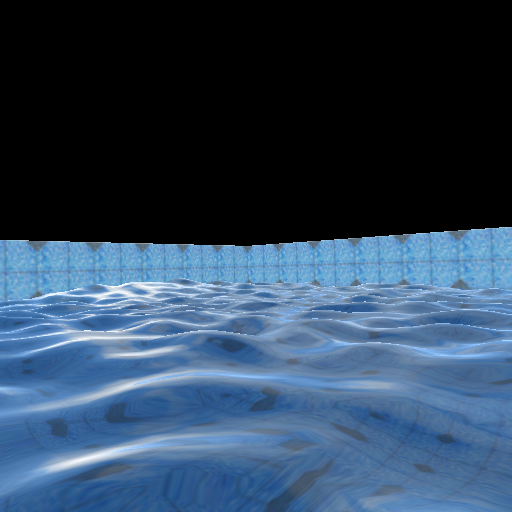
\includegraphics[scale=0.175]{figures/Towards_Real-Time_Visual_Simulation_of_Water_Surfaces_-_Schneider_2001-032.png}
	\label{fig:westermann}
 }
 \hfill
 \subtop[]%[\citeauthor{Isidoro:2002}]
 {
  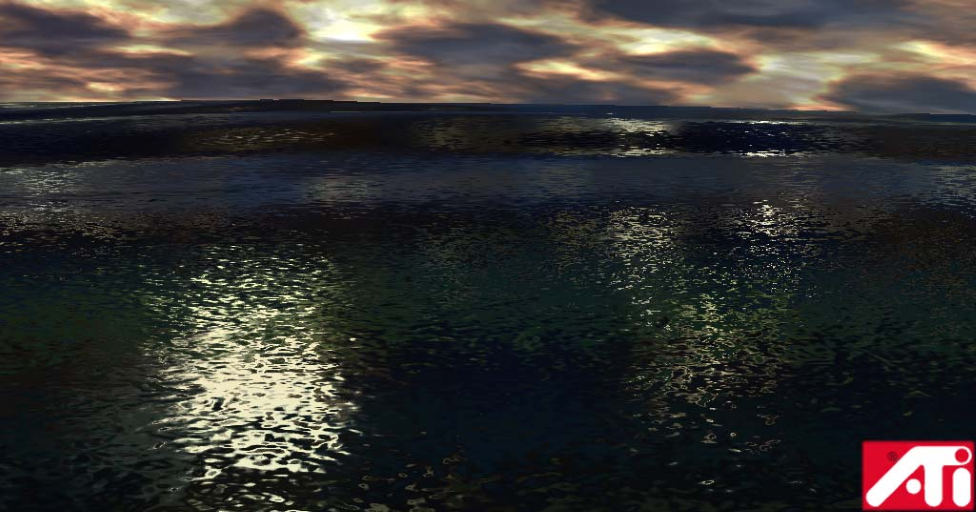
\includegraphics[scale=0.175]{figures/ShaderX_Rendering_Ocean_Water_-_Isidoro_2002-003.png}
	\label{fig:isidoro}
 }
 \hfill
 \subtop[]%[\citeauthor{Finch:2004}]
 {
  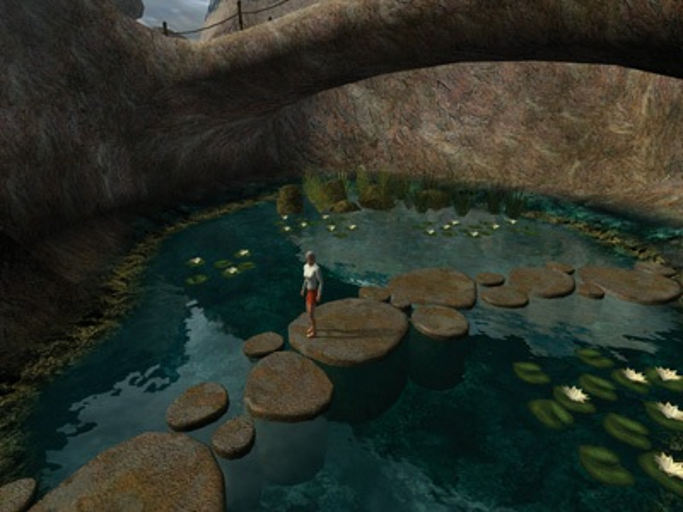
\includegraphics[scale=0.175]{figures/Effective_Water_Simulation_from_Physical_Models_-_Finch_2004-003.png}
	\label{fig:finch}
 }
 \caption{
\subcaptionref{fig:westermann} Source:~\cite{Schneider:2001}
\subcaptionref{fig:isidoro} Source:~\cite{Isidoro:2002}
\subcaptionref{fig:finch} Source:~\cite{Finch:2004}
}
\label{fig:earlygpu}
\end{figure}
%
The computer graphics community has been, and still is, hard at work to make
algorithms presented in the previous sections capable to render in real-time.
The challenge is trifold: first, the synthesis of an animated ocean surface,
second, efficient rendering of vast ocean surface geometry, and third,
believable shading of the ocean surface.

\subsection{Early Work}
Early attempts to generate plausible water surfaces on graphics hardware include
\cite{Schneider:2001, Isidoro:2002, Finch:2004}. Figure~\ref{fig:earlygpu}
depicts some of their results.
To obtain interactive framerates \citeauthor{Schneider:2001} compute the
displacements caused by wave motion using two octaves of Perlin noise in a
vertex shader on the GPU.
\citeauthor{Isidoro:2002} perturb an existing mesh by means of a sum of four
low-frequency sinusoids computed in a vertex shader on the GPU. Additional
high-frequency detail is obtained by scrolling static normalmaps across the
displaced surface.
%In a similar fashion,
%\cite{Chen:2007} employ a sum of four sinusoids to displace an existing mesh,
%and a dynamically generated normalmap to obtain more detailed surface normals.
\citeauthor{Finch:2004} uses a sum of four Gerstner waves to displace an existing
mesh, where wavelengths that are too short to be represented by the mesh are
filtered out automatically. Moreover, \citeauthor{Finch:2004} evaluates an
additional sum, with more waves involved, to generate better detailed surface
normals.

%\cite{Salgado:2007} present a simplified implementation of \cite{Fournier:1986}
%using vertex shaders.

\subsection{Adaptive Schemes}
Viewing situations involving an ocean surface are varied, from close-ups where
one may notice ripples on the surface to views where the water surface may
span until the horizon. Hence, to improve performance and visual fidelity,
it is beneficial for rendering algorithms to focus on regions near the camera
position, minimizing the number of samples according to distance from the
viewpoint.
%Given a viewing situation where one observes the ocean reaching the horizon, a
%meshing scheme with uniformly spaced vertices in world space may do us a
%disservice. The visible surface area is large and a high resolution is
%needed in regions close to the camera, thus a very large mesh is required.
%
%Minimize the sampling of the geometry according to distance from the viewpoint.
%Mesh adapts to viewing situation
%Simulation adapts to viewing situation
\begin{figure}
 \centering
 \subtop[]%[\citeauthor{Schneider:2001}]
 {
  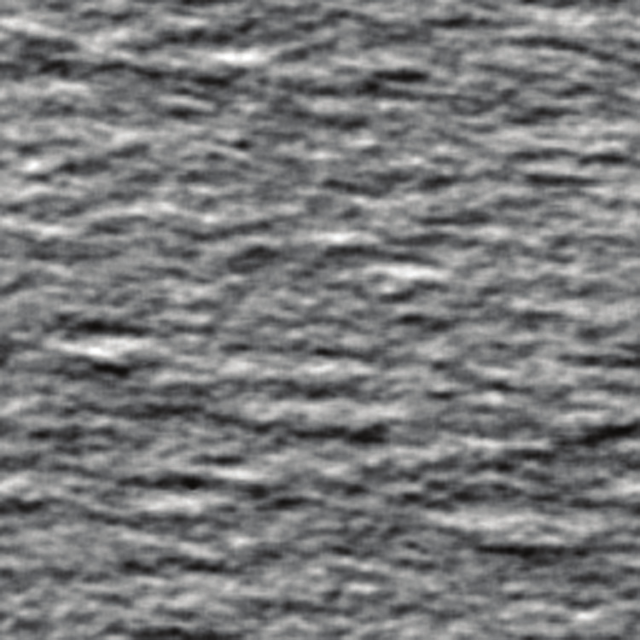
\includegraphics[scale=0.175]{figures/Using_Vertex_Texture_Displacement_for_Realistic_Water_Rendering_-_Kryachko_2005-009.png}
	\label{fig:kryachko:waves}
 }
 \hfill
 \subtop[]%[\citeauthor{Schneider:2001}]
 {
  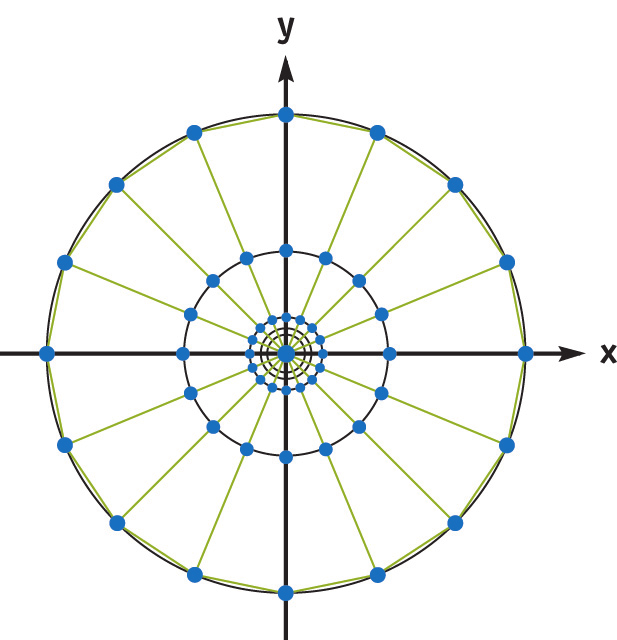
\includegraphics[scale=0.175]{figures/Using_Vertex_Texture_Displacement_for_Realistic_Water_Rendering_-_Kryachko_2005-012.png}
	\label{fig:kryachko:meshing}
 }
 \hfill
 \subtop[]%[\citeauthor{Isidoro:2002}]
 {
  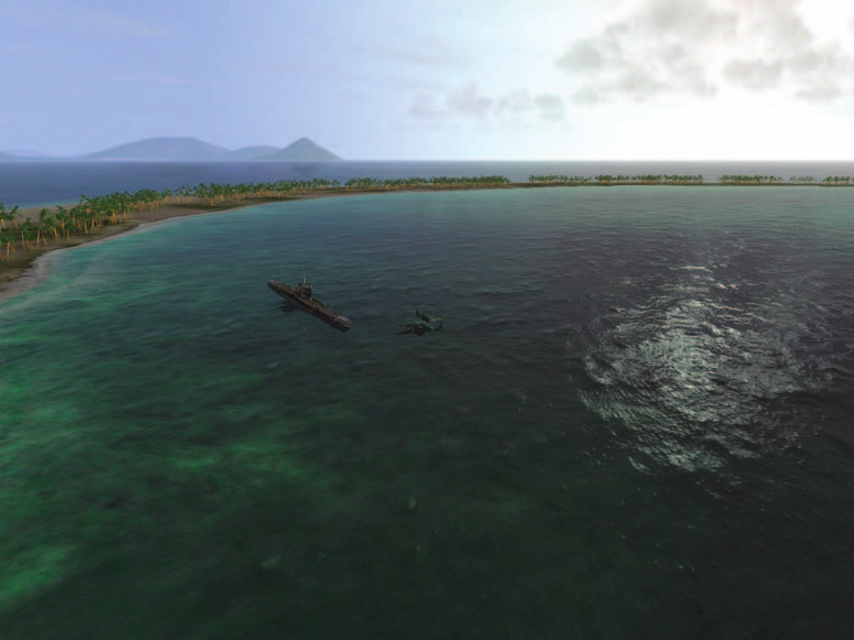
\includegraphics[scale=0.175]{figures/Using_Vertex_Texture_Displacement_for_Realistic_Water_Rendering_-_Kryachko_2005-026.png}
	\label{fig:kryachko:results}
 }
 \caption{
  \subcaptionref{fig:kryachko:waves} A height map used for water displacement.
  \subcaptionref{fig:kryachko:meshing} Radial grid centered at the camera position.
  \subcaptionref{fig:kryachko:results} View with the ocean spanning to the horizon.
  Source:~\cite{Kryachko:2005}
}
\label{fig:kryachko}
\end{figure}
%

\cite{Kryachko:2005} describes the algorithm used in an actual flight simulator.
The ocean is modeled as a combination of handcrafted heightmaps tiled in space
and time. Four heightmaps are summed for lighting computations, where the two of them
with the largest scale are used to displace the ocean surface mesh. The latter is
organized as a radial grid centered at the camera position, tesselated such that
it provides more detail close to the viewer, see Figure~\ref{fig:kryachko:meshing}.
Radial grid positions are calculated in the vertex shader, as are displacements,
allowing the algorithm to adapt the mesh vertices as well as displacement computations
to the camera position automatically on the GPU for each frame. Still, one may
notice that most of the radial mesh is alway outside the view frustum,
causing unnecessary overhead.
%
%
\begin{figure}
 \centering
 \subtop[]
 {
  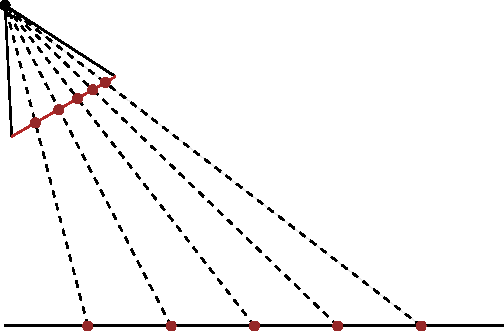
\includegraphics[scale=0.425]{figures/ProjectedGrid_UniformWS.pdf}
  \label{fig:hinsinger:projectedgrid:ws}
 }
 \hfill
 \subtop[]
 {
  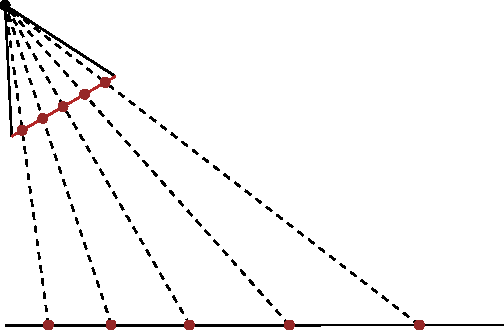
\includegraphics[scale=0.425]{figures/ProjectedGrid_UniformSS.pdf}
  \label{fig:hinsinger:projectedgrid:ss}
 }
 \hfill
 \subtop[]
 {
  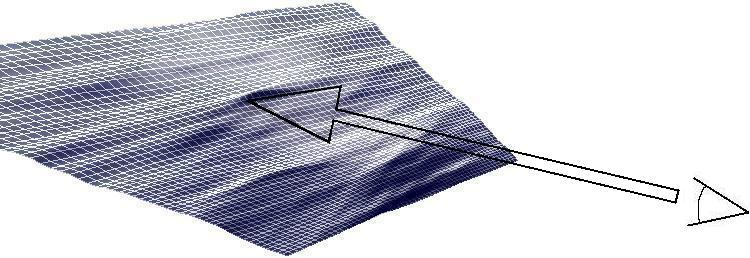
\includegraphics[scale=0.25]{figures/Interactive_Animation_of_Ocean_Waves_-_Hinsinger_2002-003.png}
  \label{fig:hinsinger:projectedgrid:mesh}
 }
 \caption{
  \subcaptionref{fig:hinsinger:projectedgrid:ws} Uniformly spaced vertices in world space, their projection onto the screen is not uniformly spaced though.
  \subcaptionref{fig:hinsinger:projectedgrid:ss} Uniformly spaced vertices in screen space projected onto world space base plane.
  \subcaptionref{fig:hinsinger:projectedgrid:mesh} The result mesh obtained by projection of the vertices onto the base plane followed by displacement.
  One can see that the surface patches grow with distance from the viewer.
  Source:~\cite{Hinsinger:2002}
}
\label{fig:hinsinger:mesh}
\end{figure}
%
%

\cite{Hinsinger:2002} present a more holistic approach, with their contribution
being twofold. One, an adaptive meshing scheme, and two, an adaptive simulation
scheme. The basic idea for the adaptive surface mesh is to make sure that every
surface element at rest covers the same area on screen. Thus, the screen is
subdivided into quads which are projected onto the plane which represents the
ocean surface at rest, see Figure~\ref{fig:hinsinger:mesh}. The result is
a mesh which automatically adapts to the current camera position and gives more
detail close to the viewer.
\citeauthor{Hinsinger:2002} synthesize waves as a sum of Gerstner waves, where
the vertices represent the sampling points. Derivatives are computed analytically
for each vertex, resulting in better normal vectors than a finite differences
approach would produce. To reduce aliasing as well as to save computation time,
wavetrains smaller than a grid quad are removed from the sum of waves for that quad.
% Visual artifacts caused by sampling locations changing with camera movement are
% hidden by the waves animation.
% First, quads in screenspace, projected onto undisturbed surface plane
% change mesh in screenspace to focus on details in certain regions
% water animation hides artifacts caused by moving vertices
% sum of gerstner waves, hand picked, not automatically from spectrum
% analytical derivatives for normals
% prune wavetrains smaller than the grid quads, fade them out
% evaluate surface at any deseired location
% no cyclicity, if ratios between wavelengths irrational
\cite{Cui:2004} uses the adaptive mesh by \citeauthor{Hinsinger:2002} for a marine
simulator with three adjacent viewports, the wave model although is a simple sum
of sinusoids with a small number of waves picked from a wave spectrum.
\cite{thesis:johanson} on the other hand improves upon the adaptive mesh of
\citeauthor{Hinsinger:2002}. First, the projection of the mesh onto the base plane
is done in a vertex shader on the GPU. Second, \citeauthor{thesis:johanson} makes
sure that the projection of the vertices works correctly in all possible viewing
situations.
%
%
\begin{figure}
 \centering
 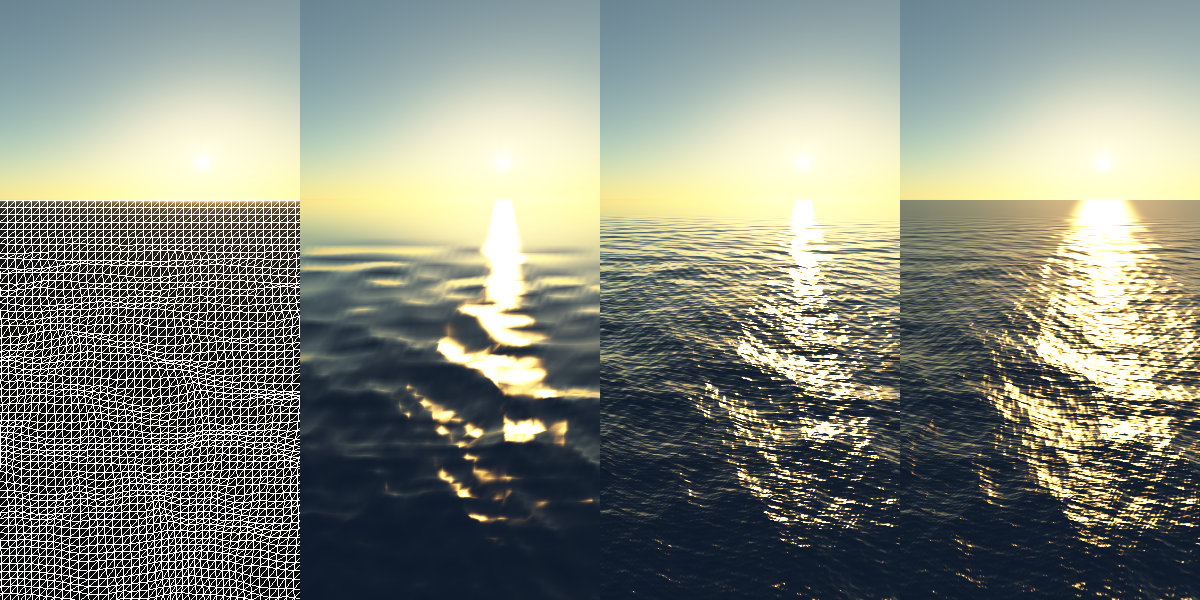
\includegraphics[scale=0.3]{figures/Seamless_Ocean_Lighting_-_Bruneton_2010-001.png}
 \caption{From left to right: The displaced surface mesh in screen space, lighting
 with geometry only, lighting with geometry and per pixel normals, lighting with 
 geometry and per pixel normals and BRDF.
 Source:~\cite{article:oceanlighting}}
\label{fig:bruneton:transitions}
\end{figure}
%
%
\begin{figure}
 \centering
 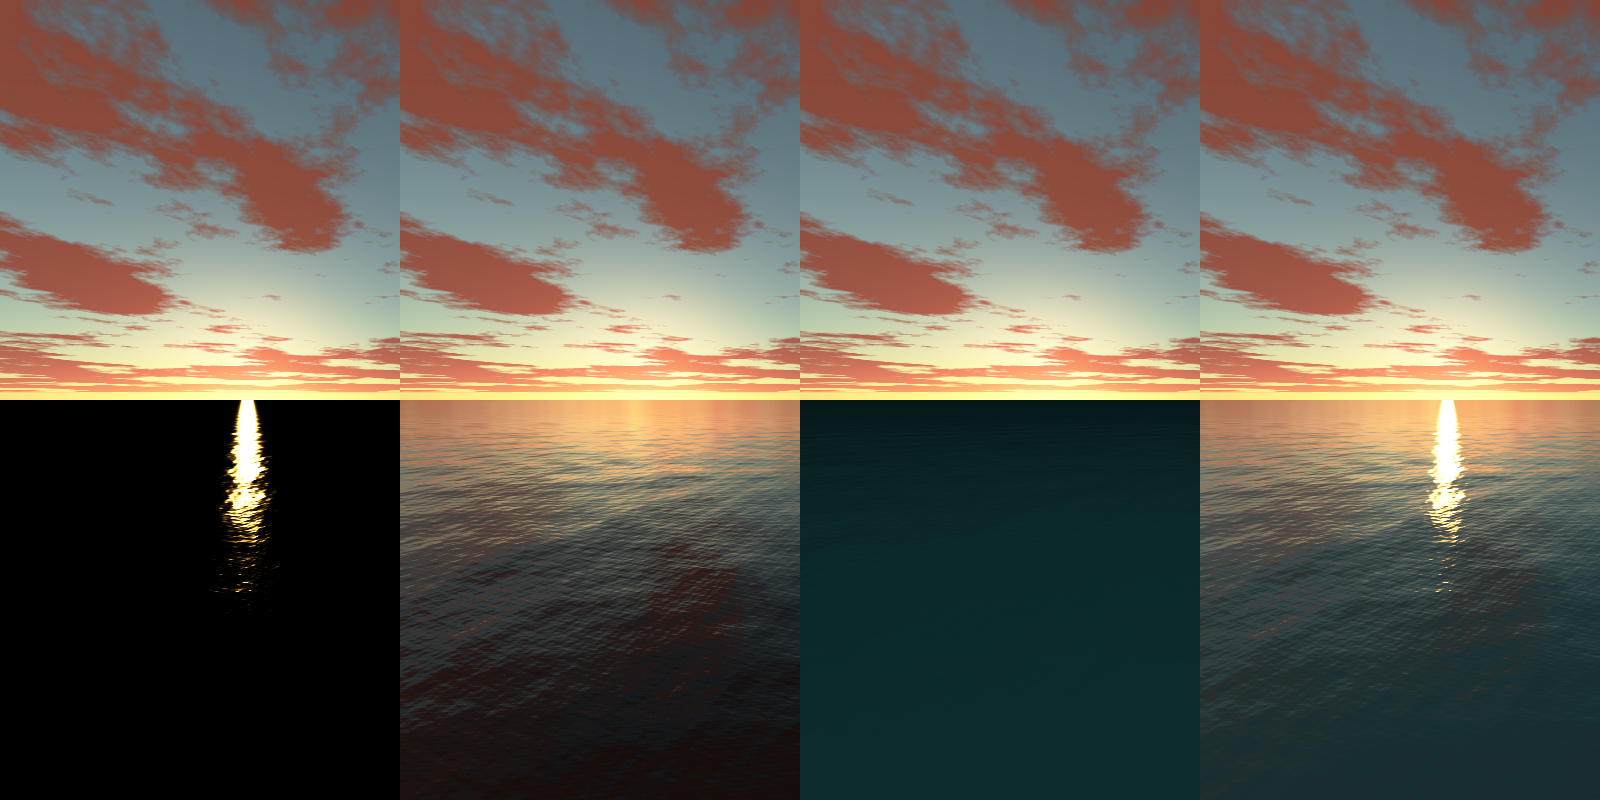
\includegraphics[scale=0.25]{figures/Seamless_Ocean_Lighting_-_Bruneton_2010-002.png}
 \caption{From left to right: The reflected sun light, the reflected sky light,
 the light refracted from the water, and the final result.
 Source:~\cite{article:oceanlighting}}
\label{fig:bruneton:lightingterms}
\end{figure}
%
%

\citet{article:oceanlighting} augment the work of \citeauthor{Hinsinger:2002} in
various areas, the most prominent improvement being an adaptive lighting scheme.
The latter is based on a hierarchical representation which combines geometry,
normals and a BRDF~\citep{Ross:2005}, where the BRDF is specifically tailored to
the statistical properties of ocean surfaces. Based on distance from the viewer,
the algorithm transitions seamlessy from lighting computed with geometry and per
pixel normals to lighting computed based solely on the statistical distribution
of ocean surface slopes as modeled by the BRDF, see Figure~\ref{fig:bruneton:transitions}.
To save computation time for vertex positions, wavetrains are filtered according
to the size of their associated projected grid cell in world space.
For the gradient computation in the pixel shader there is an additional step,
where wavetrains are filtered according to the projected size of the current pixel
in world space. In addition, \citeauthor{article:oceanlighting} show the
integration of the BRDF by \citeauthor{Ross:2005} into the computation of
all necessary lighting terms, namely the reflected light from the sun and from
the skydome, and the refracted light from the water, see
Figure~\ref{fig:bruneton:lightingterms}.
 
% Realistic animation and rendering of the ocean is an important aspect for simulators, movies and video games.
% By nature, the ocean is a difficult problem for Computer Graphics: it is a dynamic system, it combines wave trains
% at all scales, ranging from kilometric to millimetric. Worse, the ocean is usually viewed at several distances, from
% very close to the viewpoint to the horizon, increasing the multi-scale issue, and resulting in aliasing problems. The
% illumination comes from natural light sources (the Sun and the sky dome), is also dynamic, and often underlines
% the aliasing issues. In this paper, we present a new algorithm for modelling, animation, illumination and rendering
% of the ocean, in real-time, at all scales and for all viewing distances. Our algorithm is based on a hierarchical
% representation, combining geometry, normals and BRDF. For each viewing distance, we compute a simplified
% version of the geometry, and encode the missing details into the normal and the BRDF, depending on the level of
% detail required. We then use this hierarchical representation for illumination and rendering. Our algorithm runs
% in real-time, and produces highly realistic pictures and animations.

Parametric approaches in the spatial domain profit from the fact
that for each frame only visible parts and frequencies of the ocean surface
are to be evaluated. \citet{Mitchell:2005} and \citet{Thon:2000}
argue that from an algorithmic point of view one should choose a spectral
approach and leverage the highly efficient Fast Fourier Transform algorithm
to compute the sum of waves. \citeauthor{Mitchell:2005} describes a
partial GPU implementation of the ocean wave generation method presented in
\citet{course:simulatingocean}. To improve rendering performance,
\citeauthor{Mitchell:2005} synthesizes two water surface height maps,
where one contains low frequency waveforms and the other contains
low frequency and high frequency waveforms. The low frequency map
is of low resolution and is used to displace the water surface mesh.
The high resolution map is used to generate a normal map for shading.
The result is an ocean surface which appears highly detailed
while the underlying mesh is coarse.

%
%
\begin{figure}
 \centering
 \renewcommand{\thesubfigure}{}% no subfigure number
 \tightsubcaptions % we want tight subcaptions
 \setlength{\subfloatlabelskip}{0pt}% no space between number and caption
 \subtop[]
 {
  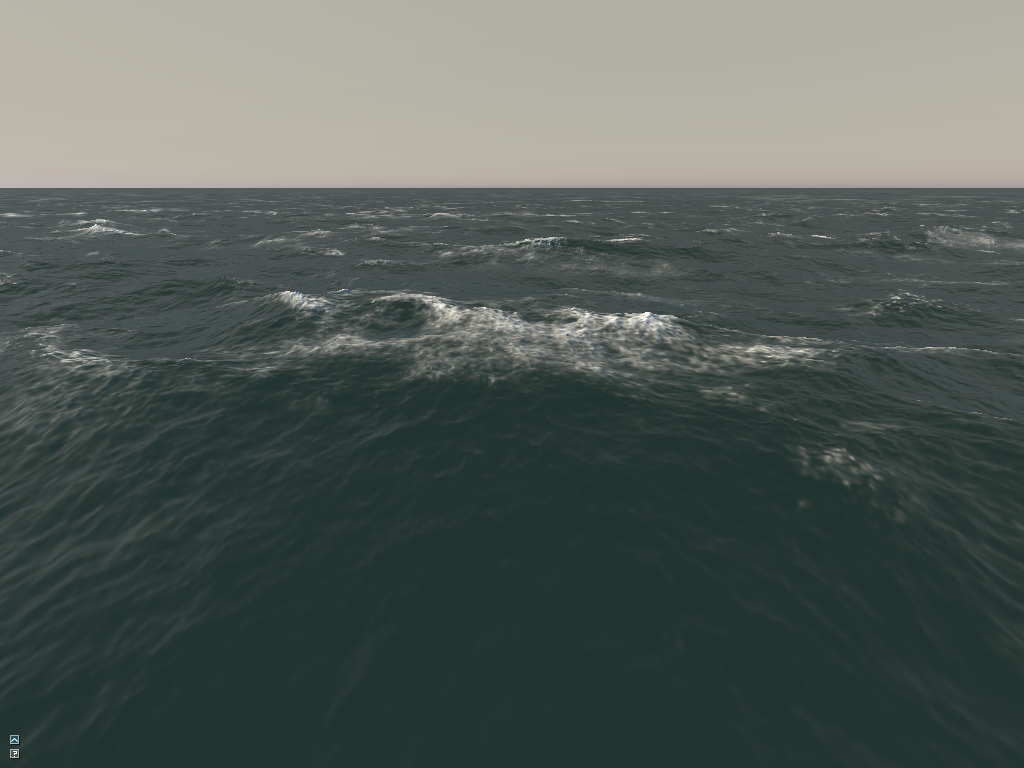
\includegraphics[scale=0.125]{figures/Real-time_Animation_and_Rendering_of_Ocean_Whitecaps-000.png}
  %\label{fig:hinsinger:projectedgrid:ws}
 }
 \hfill
 \subtop[]
 {
  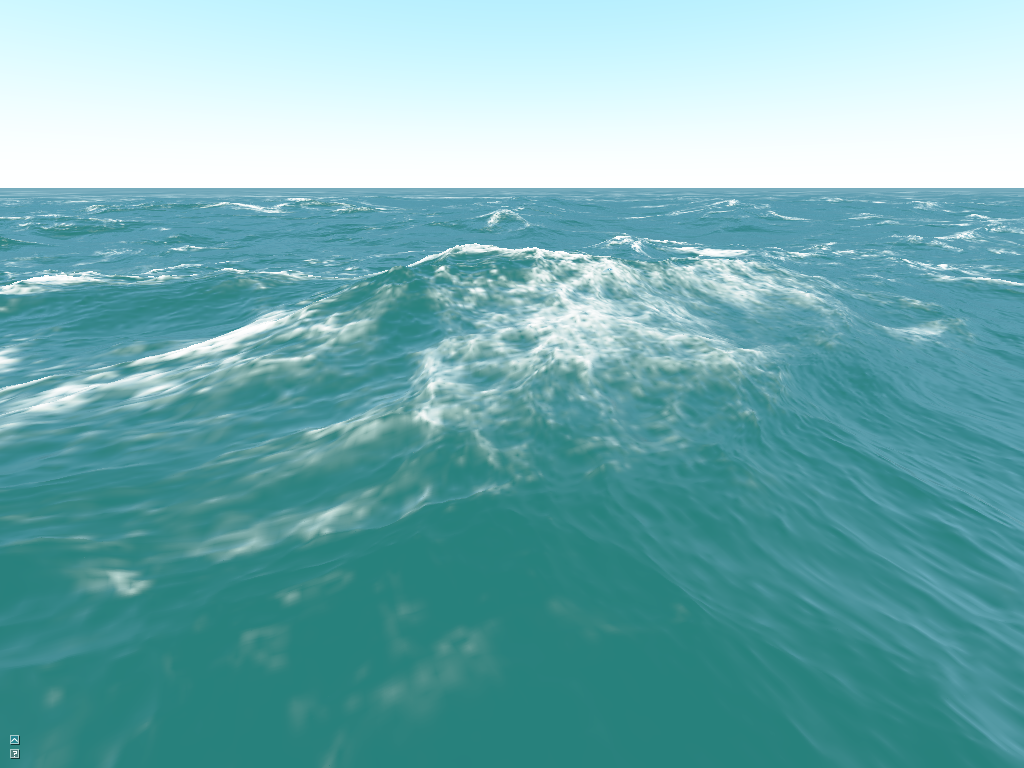
\includegraphics[scale=0.125]{figures/Real-time_Animation_and_Rendering_of_Ocean_Whitecaps-002.png}
  %\label{fig:hinsinger:projectedgrid:ss}
 }
 \hfill
 \subtop[]
 {
  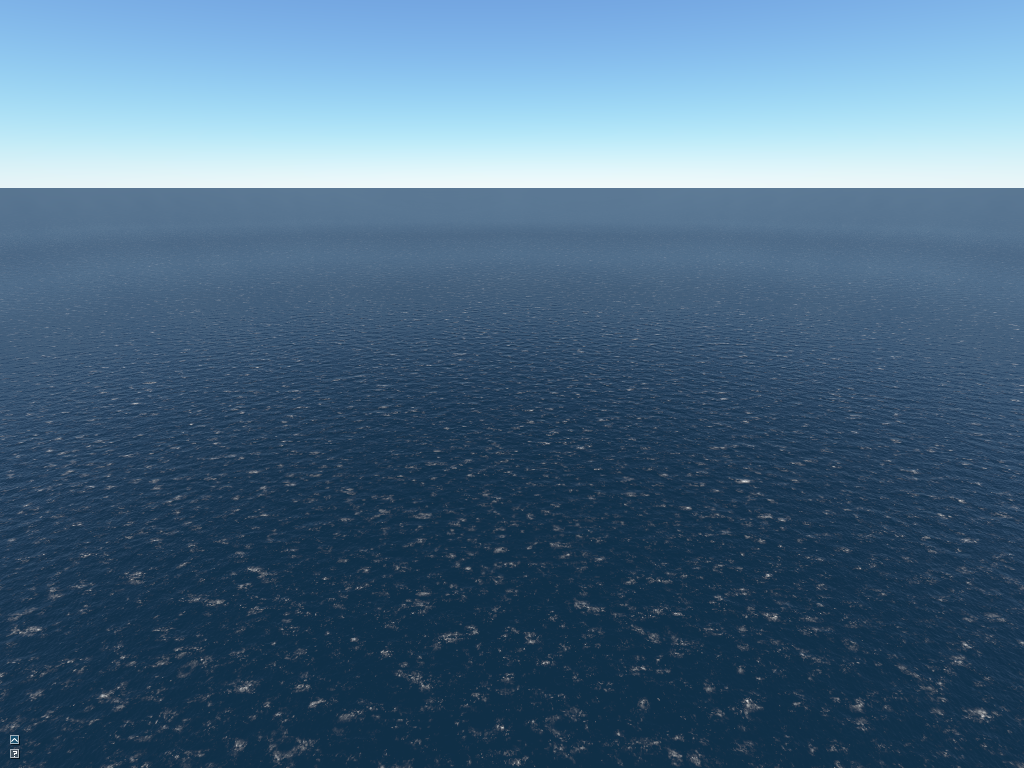
\includegraphics[scale=0.125]{figures/Real-time_Animation_and_Rendering_of_Ocean_Whitecaps-004.png}
  %\label{fig:hinsinger:projectedgrid:mesh}
 }
\caption{A set of example ocean scenes with whitecaps. Source:~\cite{article:whitecaps}
}
\label{fig:dupuy:whitecaps}
\end{figure}
%
%
\citet{misc:oceanlightingfft} combines the adaptive lighting scheme
from \citet{article:oceanlighting} with an ocean surface synthesized
from the wave spectrum presented in~\citet{article:Elfouhaily1997}.
Wave heights, gradients, as well as the horizontal displacements
required for~\citeauthor{course:simulatingocean}'s choppy wave algorithm
are computed entirely on the GPU. In an additional step,
\citet{article:whitecaps} add whitecaps to the ocean lighting model,
see Figure~\ref{fig:dupuy:whitecaps}.

As ocean surfaces generated from wave spectra allow for seamless tiling,
one may need to make sure to reduce tiling artifacts i.e. the viewer
shall not notice that the ocean surface repeats itself in all directions.
The approach taken by~\citet{Rydahl:2009} and \citet{NVIDIA:Ocean} is to
generate additional noise on the ocean surface.
\citet{misc:oceanlightingfft,article:whitecaps}
on the other hand compute not just one ocean surface tile, but up to four,
where all tiles are of different size and each one samples a different
part of the wave spectrum. Even though such an approach is unable to
entirely remove periodicity, the period is increased to the least common
multiple of the different tile sizes.


%%%%%%%%%%%%%%%%%%%%%%%%%%%%%%%%%%%%%%%%%
%%%%%%%%%%%%%%%%%%%%%%%%%%%%%%%%%%%%%%%%%

%\section{The Projected Grid}
The projected grid is based on a simple concept: in order to achieve an
uniform distribution of details on the image plane, a uniformly spaced grid is
created in post-perspective space and transformed back to world space.
Figure~\ref{fig:projectedgrid} illustrates the difference between a classic
world space approach and the projected grid.
\begin{figure}[h]
\centering
\subbottom[Increase]
{
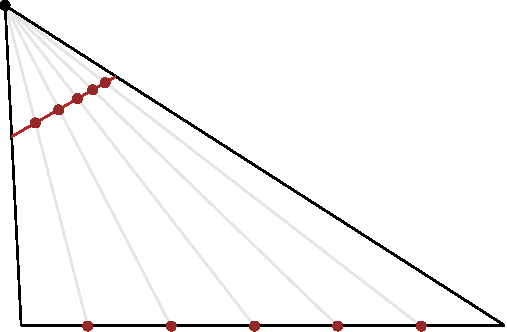
\includegraphics[scale=0.75]{figures/ProjectedGridVsWorldSpace.pdf}
\label{fig:subfigprojgrid1}
}
\subbottom[Increase]
{
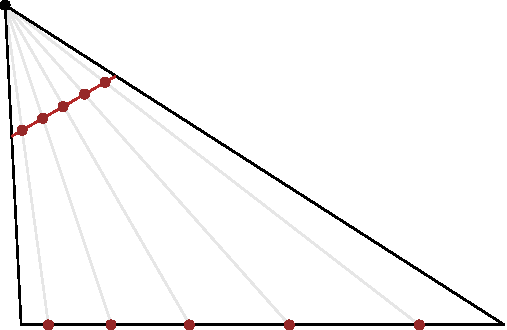
\includegraphics[scale=0.75]{figures/ProjectedGridUniform.pdf}
\label{fig:subfigprojgrid2}
}
\caption[The Projected Grid Concept]{The image on the left shows an uniform
grid in worldspace, its projection onto the image plane is not uniformly
spaced though. The image on the right on the other hand depicts an uniform grid on
the image plane and its associated non-uniform spaced worldspace positions.}
\label{fig:projectedgrid}
\end{figure}

% The algorithm used for the projected grid can be broken down into the following
% steps:
% \begin{itemize}
%  \item create a uniformly spaced grid orthogonal to the viewer using normalised
% device coordinates
%  \item transform the grid to worldspace
%  \item project the grid onto the desired base plane
%  \item apply height displacement
%  \item run the grid through the rendering pipeline as usual
% \end{itemize}

\newcommand{\mvec}[1]{\mathbf{#1}}
\newcommand{\mvecx}[1]{\mathbf{#1}_x}
\newcommand{\mvecy}[1]{\mathbf{#1}_y}
\newcommand{\mvecz}[1]{\mathbf{#1}_z}
\newcommand{\mvecw}[1]{\mathbf{#1}_w}
\newcommand{\mmat}[1]{\mathbf{#1}}
\newcommand{\transpose}[1]{#1^{\mathsf{T}}}
\newcommand{\inverse}[1]{#1^{\mathsf{-1}}}

Let $\mvec{x}$ be a vector representing the three dimensional carthesian
world space coordinate of a vertex, then
\begin{equation}
 \mvec{w} = \transpose{(\mvecx{x}, \mvecy{x}, \mvecz{x}, 1)}
\end{equation}
where $\mvec{w}$ is a homogeneous world space coordinate of $\mvec{x}$.
Let $\mmat{V}$ be the view matrix and $\mmat{P}$ the projection matrix, then
\begin{equation}
\label{eq:ws_to_cs}
 \mvec{c} = \mmat{P} \mmat{V} \mvec{w}
\end{equation}
where $\mvec{c}$ is the \textit{clip space} coordinate of $\mvec{w}$. For $\mvec{c}$ to
be inside the view frustum defined by $\mmat{P}$, $\mvec{c}$ is required to
meet the following condition
\begin{equation}
\label{eq:cs_bounds}
 \mvecx{c}, \mvecy{c}, \mvecz{c} \in \interval{-\mvecw{c}}{\mvecw{c}}
\end{equation}
where $\mvecw{c}$ is the homogeneous component of $\mvec{c}$. Next, clip space
vertex $\mvec{c}$ is transformed by the \textit{perspective division} as follows
\begin{equation}
\label{eq:cs_to_ndc}
 \mvec{n} = \frac{1}{\mvecw{c}}\transpose{(\mvecx{c}, \mvecy{c}, \mvecz{c})}
\end{equation}
where $\mvec{n}$ corresponds to the \textit{normalised device coordinate},
\textit{NDC} in short, of $\mvec{c}$. As one can see, equations~\ref{eq:cs_bounds}
and~\ref{eq:cs_to_ndc} imply
\begin{equation}
\label{eq:ndc_bounds}
 \mvecx{n}, \mvecy{n}, \mvecz{n} \in \interval{-1}{1}
\end{equation}
which defines the space NDC reside in, namely the \textit{canonical view volume},
a three dimensional cube centered at the origin, with a side length equal two.\\


The projected grid, on the other hand, starts inside the canonical view volume
and needs to transform vertices back to world space. Let $\mvec{n}$ be the
normalised device coordinate of a vertex, then
\begin{equation}
\label{eq:ndc_to_cs}
 \mvec{c} = \transpose{(\mvecx{n}, \mvecy{n}, \mvecz{n}, 1)}
\end{equation}
where $\mvec{c}$ is a valid representation of $\mvec{n}$ in clip space. One may choose
a value for $\mvecw{c}$ different from $1$, making it necessary to scale $\mvecx{n}$,
$\mvecy{n}$ and $\mvecz{n}$ accordingly. Again, let $\mmat{V}$ be the view matrix and
$\mmat{P}$ the projection matrix, then
\begin{equation}
\label{eq:cs_to_wsh}
 \mvec{w} = \inverse{(\mmat{P} \mmat{V})} \mvec{c}
\end{equation}
where $\mvec{w}$ is a homogeneous world space coordinate of $\mvec{c}$. Conversion
to three dimensional carthesian world space is accomplished as follows
\begin{equation}
\label{eq:wsh_to_ws}
 \mvec{x} = \frac{1}{\mvecw{w}}\transpose{(\mvecx{w}, \mvecy{w}, \mvecz{w})}
\end{equation}

To simplify matters the grid may be consist of vertices defined by
two-dimensional normalised device coordinates. In order to project the grid
onto a plane a ray has to be setup for every vertex.

postprojection coordinates transformed to worldspace
grid on near and far plane, intersection with the y=0 plane
decouple projector from camera


%%%%%%%%%%%%%%%%%%%%%%%%%%%%%%%%%%%%%%%%%
%%%%%%%%%%%%%%%%%%%%%%%%%%%%%%%%%%%%%%%%%

%\chapter{Implementation}
\label{ch:implementation}
%
The previous chapter discussed the wave spectrum concept, a theoretical
framework developed by oceanographic research to describe the distribution of
wave energy among ocean surface waves exposed to identical conditions, such as
wind speed and distance to shore~\citep{Neumann:1966}.
%Several wave spectrum models were introduced, where each comes with a set of conditions
%it functions under.
Based on wave spectra we are able to synthesize ocean surfaces of great variety:
from a perfectly calm sea, over one slightly agitated by the wind, to one with
massive waves caused by a storm overhead.
But to be able to visualize such diverse seas in a convincing manner we are dependent on more data
than surface elevation alone. Therefore, as described by \citet{course:simulatingocean},
we may capitalize on the spectral representation of ocean waves to obtain
three distinct additional datasets.
One, high quality normal vectors by deriving the ocean surface's slope vectors in frequency space.
Two, displacements to transform the gentle form of the sea into a more agitated one, where the waves are more similar to Gerstner waves than to sinusoids.
Three, the first-order partial derivatives of aforementioned displacements, as they allow us to deduce the locations on the ocean surface where
whitecaps may arise.
Each of the three datasets requires us to construct additional spectra,
all derived directly from the ocean surface elevation spectrum.
%Thus, we may be burdened with a significant number of additional Fourier Transforms,
%increasing the computational workload considerably.

Alongside data synthesis, it is the rendering of a water body as large as the ocean
that poses a challenge. The variety of possible camera views
may range from closeups of the water surface to vistas where the sea spans all
the way to the horizon.
In the former case we would like to be able to observe small scale detail on the
water surface, such as ripples caused by capillary waves.
The latter case is not difficult to handle in principle, because the ocean surface
data we synthesize is seamlessly tileable. Still, we would prefer that the viewer
may not be able to notice that the ocean surface repeats itself in all directions.
To tackle both issues at once, we adopt the level-of-detail approach taken by
\citet{misc:oceanlightingfft} and \citet{article:whitecaps}.
We compute a set of ocean surface tiles of differing size, where each tile samples a
different part of the wave energy spectrum. By combining the tiles we may
extend the sum of waves as far as into the gravity-capillary wave domain.
As for the tiling artifacts, even though we are unable to entirely remove periodicity
by combing multiple tiles, we are at least able to increase the period to the
least common multiple of the different tile sizes.

As one may already guess, we are burdened with a significant number of
\FourierTransforms, based on both the number of spectra per tile (surface elevation,
slopes, displacements, first order derivatives of the displacements),
and the number of different tiles.
Thus, we need to make sure to keep computational workload on an acceptable level
for realtime display of the ocean. We chose to go about the issue at hand in a
twofold manner.
First, key properties of the ocean surface spectrum allow us to accelerate the
computation of its \InvFourierTransform considerably.
Second, we reduce the amount of spectral data to transform. We achieve the
latter by improving upon the level-of-detail approach by \citet{misc:oceanlightingfft}
and \citet{article:whitecaps} with a multi-resolution scheme, where surface
elevation and displacements are generated at a lower resolution
than their respective first-order derivates.
%, where certain spectra are of lower resolution than others.
%Twofold, first accelerate Fourier Transform, second, multiresolution approahc for ocean data.

%In the former case one should be able to observe small scale detail such as
%ripples on the water surface, where in the latter case the viewer
%shall not be able to notice that the ocean surface repeats itself in all directions.
%To tackle both issues at once, we adopt the approach taken by \citet{misc:oceanlightingfft}
%and \citet{article:whitecaps}.
%We compute a set of ocean surface tiles of differing size, where each tile samples a
%different part of the wave energy spectrum. By combining the tiles we may
%extend the sum of waves as far as into the gravity-capillary wave domain.
%And, even though we are unable to entirely remove periodicity, the period is
%increased to the least common multiple of the different tile sizes.

% In the former
% case one should be able to observe small scale detail on the water surface, therefore
% it is beneficial for the wave spectrum to extend even as far as into the
% gravity-capillary wave domain. In principle, we are able to handle the latter case
% without issues, because the data we synthesize is seamlessy tileable. Still, one
% should not be able to notice that the ocean surface repeats itself in all directions.

%Furthermore, to add level of detail and to reduce tiling artifacts,
%we adopt the approach taken by \citet{misc:oceanlightingfft} and
%\citet{article:whitecaps}. We compute and combine a set of ocean surface tiles
%of differing size, where each tile samples a different part of the wave energy
%spectrum.
%Thus, we are potentially burdened with a significant number of additional
%Fourier Transforms, based on both the number of additional spectra per tile,
%and the number of different tiles.

%Specific properties of said models allow for
%easy addition and reduction of detail, as well as for a range of algorithmic
%optimisations. The former combined with the latter gives us the opportunity to
%strike a well-adjusted balance between model detail and computational workload,
%and thereby to improve upon the status quo of current implementations.
%
%Rendering an ocean is a demanding task for several reasons. First, consider the
%sheer size of a water body as large as an ocean, which in numerous viewing
%situations will be visible all the way to the horizon.
%
%The remainder of this work is organized as follows: Chapter
%\ref{ch:state_of_the_art} gives a survey of existing ocean simulation and
%rendering methods. Chapter~\ref{ch:background} elaborates on the theoretical
%background the oceanographic models are based on, as well as on the models
%themselves. Chapter~\ref{ch:implementation} describes in detail the
%synthesis of all data related to the ocean surface, including both the algorithmic
%optimisations and the level of detail mechanism. Furthermore, we give an overview
%of the rendering algorithms adopted for our implementation.

%up to four, where all tiles are of different size and each one samples a different
%part of the wave spectrum.

%As ocean surfaces generated from wave spectra allow for seamless tiling,
%one may need to make sure to reduce tiling artifacts i.e. the viewer
%shall not notice that the ocean surface repeats itself in all directions.
%The approach taken by~\citet{Rydahl:2009} and \citet{NVIDIA:Ocean} is to
%generate additional noise on the ocean surface.
%\citet{misc:oceanlightingfft} and \citet{article:whitecaps}
%on the other hand compute not just one ocean surface tile, but up to four,
%where all tiles are of different size and each one samples a different
%part of the wave spectrum. Even though such an approach is unable to
%entirely remove periodicity, the period is increased to the least common
%multiple of the different tile sizes.

%All three points lead to additional spectra, all derived directly from the ocean
%surface elevation spectrum, burdening us with additional Fourier Transforms.

%But a sea exposed to strong
%winds or even a storm is characterized by steep waves with sharp crests.
%\citet{course:simulatingocean} presents the~\emph{choppy wave} algorithm which
%overcomes this specific issue by allowing the waves to take a form similar to
%Gerstner waves, with deep troughs and sharp crests, see Figure
%\ref{fig:tessendorf_choppy_waves}.
%to obtain
%additional high quality data to improve the geometry of the ocean surface.
%Moreover, \citet{misc:oceanlightingfft} implements a wave spectrum based
%version of \citet{article:oceanlighting}, serving us as lighting algorithm.
%\citet{article:whitecaps}
%
%All additional data is derived directly from the ocean surface elevation
%spectrum in frequency space, burdening us with additional Fourier Transforms.

%The previous chapter gave us conceptual background regarding wave spectra,
%Although the general shape and movement of the ocean surface waves may be already
%sufficiently plausible to the observer's eye, there is still room for improvement.


%In the previous chapter we discussed the synthesis of ocean surfaces based
%on wave spectra published in oceanographic research.
%
%At this point we know how to synthesize ocean surfaces based on wave spectra
%from oceanographic research. We may move on to how to optimally employ them in the
%cpntext of computer graphics. 
%representaiotn of wave spectra most suitable for rendering
%obtain all data necessary for rendering from wave spectra

%At this point we are able to synthesize ocean surfaces in the form of simple
%heightfields animated over time.
%Although the shape of the ocean surface waves as well as their movement
%may be already sufficiently plausible to the observers eye, 
%The shape of the ocean surface waves, as well as their
%movement are sufficiently plausible to the observers eye.

%For rendering purposes we will augment our ocean surface representation with
%additional data as described by \citet{course:simulatingocean}.

%One, a displacement vector field which modifies the gentle sinusoidal form of the
%waves into one with deeper troughs and sharper crests, similar to Gerstner waves.
%Two, high-quality normals for detailed lighting.
%Three, the Jacobian matrix of the displacement vector field,
%
 %two, a displacement vector field which allows
%for steep waves with sharp crests, and three, the Jacobian of the displacement
%vector field
%\citep{course:simulatingocean}.
%
%with the choppy-wave algorithm (Tessendorf).
%
%\cite{course:simulatingocean,article:oceanlighting,misc:oceanlightingfft,article:whitecaps}

The remainder of this chapter is organized as follows:
Section~\ref{sec:spectrum_synthesis} gives a compact summary of ocean surface
synthesis by means of a wave energy spectrum.
Section~\ref{sec:discrete_fourier_transform} describes characteristic properties of
wave spectra which enable us to accelerate the computation of the \InvFourierTransform.
Section~\ref{sec:slopes_and_displacements} introduces the additional wave spectrum
based datasets which we employ for rendering, whereas
Section~\ref{sec:level_of_detail} elaborates on our wave spectrum specific
approach to level of detail. Last, Section~\ref{sec:demo_application} gives an
overview of our demo application and the algorithms it incorporates.

%Ocean surfaces based on wave spectra all share the same issue, namely the all to
%gentle form of wave troughs and wave crests. Because the surface is computed as
%a linear superposition of sinusoids, it is only natural that the result shares
%the general form of its underlying building blocks. But a sea exposed to strong
%winds or even a storm is characterized by steep waves with sharp crests.
%\citet{course:simulatingocean} presents the~\emph{choppy wave} algorithm which
%overcomes this specific issue by allowing the waves to take a form similar to
%Gerstner waves, with deep troughs and sharp crests, see Figure
%\ref{fig:tessendorf_choppy_waves}.


%Section~\ref{sec:discrete_fourier_transform} describes opportunities to optimize
%the computation of the DFT which arise due to specific properties of wave spectra.
%Section~\ref{sec:slopes_and_displacements} discusses additional terms derived
%from the wave spectrum representation to enhance lighting as well as allow for
%more geometrical variety of the ocean surface.
%Section~\ref{sec:level_of_detail} delineates the level of detail
%approach we took to balance model detail and computational workload.
%
%Section~\ref{sec:level_of_detail} delineates one, the approach we took to assemble the wave spectrum from \wavevector
%domains which complement each other, and two, a simple procedure which allows for
%differing resolutions for all terms related to, and the wave spectrum itself.
%dft and how to exploit it
%
%spectrum and data derived from it (normals, displacements)
%level of detail (sampling of different parts of spectrum, multi-resolution spectrum)



%\section{The Projected Grid}
%\label{sec_projected_grid}
%The projected grid is based on a simple concept: in order to achieve an
%uniform distribution of details on the image plane, a uniformly spaced grid is
%created in post-perspective space and transformed back to world space.
%Figure~\ref{fig:projectedgrid} illustrates the difference between a classic
%world space approach and the projected grid.
%\begin{figure}[h]
%\centering
%\subbottom[Classic]
%{
%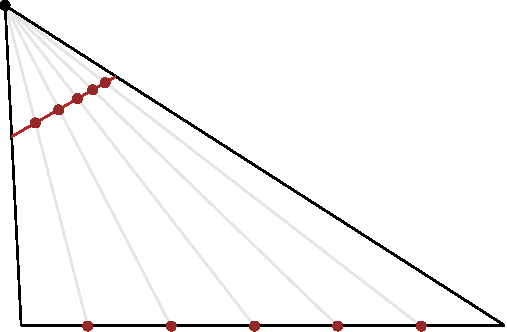
\includegraphics[scale=0.75]{figures/ProjectedGridVsWorldSpace.pdf}
%\label{fig:subfigprojgrid1}
%}
%\subbottom[Projected Grid]
%{
%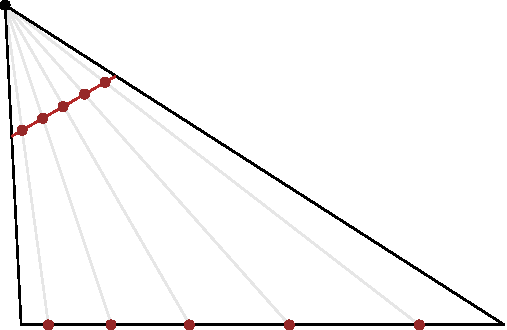
\includegraphics[scale=0.75]{figures/ProjectedGridUniform.pdf}
%\label{fig:subfigprojgrid2}
%}
%\caption{The image on the left shows an uniform grid in worldspace,
%its projection onto the image plane is not uniformly spaced though.
%The image on the right on the other hand depicts an uniform grid on
%the image plane and its associated non-uniform spaced worldspace
%positions.}
%\label{fig:projectedgrid}
%\end{figure}
%
%% The algorithm used for the projected grid can be broken down into the following
%% steps:
%% \begin{itemize}
%%  \item create a uniformly spaced grid orthogonal to the viewer using normalised
%% device coordinates
%%  \item transform the grid to worldspace
%%  \item project the grid onto the desired base plane
%%  \item apply height displacement
%%  \item run the grid through the rendering pipeline as usual
%% \end{itemize}
%
%\subsection{Coordinate Systems}
%\label{sec:coordinate_systems}
%Let $\mvec{x}$ be a vector representing the three dimensional carthesian
%world space coordinate of a vertex, then
%\begin{equation}
 %\mvec{w} = \transpose{(\mvecx{x}, \mvecy{x}, \mvecz{x}, 1)}
%\end{equation}
%where $\mvec{w}$ is a homogeneous world space coordinate of $\mvec{x}$.
%Let $\mmat{V}$ be the view matrix and $\mmat{P}$ the projection matrix, then
%\begin{equation}
%\label{eq:ws_to_cs}
 %\mvec{c} = \mmat{P} \mmat{V} \mvec{w}
%\end{equation}
%where $\mvec{c}$ is the \textit{clip space} coordinate of $\mvec{w}$. For $\mvec{c}$ to
%be inside the view frustum defined by $\mmat{P}$, $\mvec{c}$ is required to
%meet the following condition
%\begin{equation}
%\label{eq:cs_bounds}
 %\mvecx{c}, \mvecy{c}, \mvecz{c} \in \interval{-\mvecw{c}}{\mvecw{c}}
%\end{equation}
%where $\mvecw{c}$ is the homogeneous component of $\mvec{c}$. Next, clip space
%vertex $\mvec{c}$ is transformed by the \textit{perspective division} as follows
%\begin{equation}
%\label{eq:cs_to_ndc}
 %\mvec{n} = \frac{1}{\mvecw{c}}\transpose{(\mvecx{c}, \mvecy{c}, \mvecz{c})}
%\end{equation}
%where $\mvec{n}$ corresponds to the \textit{normalised device coordinate},
%\textit{NDC} in short, of $\mvec{c}$.
%%
%%
%\begin{figure}
%\centering
%\subbottom[View Frustum]
%{
%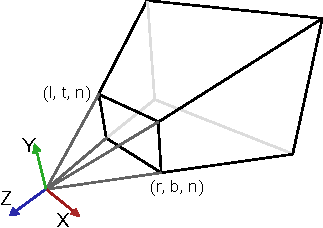
\includegraphics[width=0.4\textwidth]{figures/ProjectiveFrustum.pdf}
%\label{fig:subfig_proj_frustum}
%}
%\subbottom[Canonical view volume]
%{
%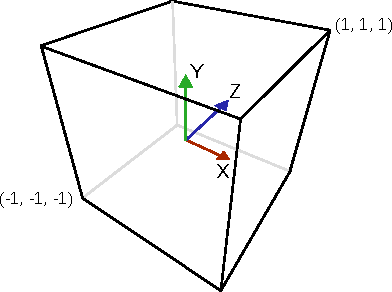
\includegraphics[width=0.4\textwidth]{figures/CanonicalCube.pdf}
%\label{fig:subfig_canonical_view_volume}
%}
%\caption{Left: An example view frustum in view space. Right: The same view frustum
%after applying projection and perspective division.}
%\label{fig:proj_frustum_ndc}
%\end{figure}
%%
%%
%As one can see, equations~\ref{eq:cs_bounds}
%and~\ref{eq:cs_to_ndc} imply
%\begin{equation}
%\label{eq:ndc_bounds}
 %\mvecx{n}, \mvecy{n}, \mvecz{n} \in \interval{-1}{1}
%\end{equation}
%which defines the space NDC reside in, namely the \textit{canonical view volume},
%see Figure~\ref{fig:proj_frustum_ndc}.\\
%
%
%The projected grid, on the other hand, starts inside the canonical view volume
%and needs to transform vertices back to world space. Let $\mvec{n}$ be the
%normalised device coordinate of a vertex, then
%\begin{equation}
%\label{eq:ndc_to_cs}
 %\mvec{c} = \transpose{(\mvecx{n}, \mvecy{n}, \mvecz{n}, 1)}
%\end{equation}
%where $\mvec{c}$ is a valid representation of $\mvec{n}$ in clip space. One may choose
%a value for $\mvecw{c}$ different from $1$, making it necessary to scale $\mvecx{n}$,
%$\mvecy{n}$ and $\mvecz{n}$ accordingly. Again, let $\mmat{V}$ be the view matrix and
%$\mmat{P}$ the projection matrix, then
%\begin{equation}
%\label{eq:cs_to_wsh}
 %\mvec{w} = \inverse{(\mmat{P} \mmat{V})} \mvec{c}
%\end{equation}
%where $\mvec{w}$ is a homogeneous world space coordinate of $\mvec{c}$. Conversion
%to three dimensional carthesian world space is accomplished as follows
%\begin{equation}
%\label{eq:wsh_to_ws}
 %\mvec{x} = \frac{1}{\mvecw{w}}\transpose{(\mvecx{w}, \mvecy{w}, \mvecz{w})}
%\end{equation}
%
%\subsection{Projection onto Plane}
%As noted before, the vertices of the projected grid are represented as normalised
%device coordinates. Assuming the plane the grid shall be projected on is specified
%in world space coordinates, the following steps need to be computed for each vertex:
%\begin{itemize}
 %\item Transform vertex from canonical view volume to world space
 %\item Setup vertex specific ray
 %\item Intersect ray with target plane to compute actual position
%\end{itemize}
%Step one is already covered by Section~\ref{sec:coordinate_systems}. Step two
%requires to setup a ray for each vertex, which implies both a position and a
%direction. The position we already have, but to create a direction we need two
%different positions. The solution is rather straightforward: let $\mvec{n}$ be
%a \textit{two-dimensional} vector representing the \textit{X} and \textit{Y}
%components of a position in normalised device coordinates, then
%\begin{align}
 %\mvec{a} & = (\mvecx{n}, \mvecy{n}, -1, 1)\\
 %\mvec{b} & = (\mvecx{n}, \mvecy{n}, +1, 1)
%\end{align}
%where $\mvec{a}$ corresponds to $\mvec{n}$ on the \textit{near plane} in clip space,
%and $\mvec{b}$ to $\mvec{n}$ on the \textit{far plane} in clip space. Let $\mvec{d}$
%and $\mvec{e}$ be the carthesian world space positions of $\mvec{a}$ and $\mvec{b}$
%respectively, then
%\begin{equation}
 %\label{eq:proj_grid_ray}
 %\mvec{p} = \mvec{d} + t(\mvec{e} - \mvec{d})
%\end{equation}
%where $\mvec{p}$ represents a ray starting at point $\mvec{d}$, pointing in direction
%$(\mvec{e} - \mvec{d})$ with variable parameter $t$ controlling the actual position on
%the ray.\\
%
%Step three is about intersecting ray $\mvec{p}$ resulting from step two with the target plane.
%We define the target plane using the \textit{Hesse normal form} as follows
%\begin{equation}
%\label{eq:proj_grid_plane}
 %\mvec{p}\transpose{\mvec{n}} - d = 0
%\end{equation}
%where $\mvec{n}$ is the plane's normal vector with unit length and $d$ the plane's distance
%from the origin. Next, we insert $\mvec{p}$ from equation~\ref{eq:proj_grid_ray}
%into equation~\ref{eq:proj_grid_plane}, resulting in
%%
%\begin{gather}
%\label{eq:plane_and_ray_intersection}
%(\mvec{d} + t(\mvec{e} - \mvec{d})\transpose{\mvec{n}} - d = 0\\
%\mvec{d}\transpose{\mvec{n}} + t(\mvec{e} - \mvec{d})\transpose{\mvec{n}} - d = 0\\
%\intertext{solve for $t$}
%t = \cfrac{d - \mvec{d}\transpose{\mvec{n}}}{(\mvec{e} - \mvec{d})\transpose{\mvec{n}}}
%\end{gather}
%%
%where $t$ in combination with equation~\ref{eq:proj_grid_ray} gives the point of intersection
%between the ray and the plane. In case $(\mvec{e} - \mvec{d})\transpose{\mvec{n}} = 0$,
%there is no point of intersection because the ray is parallel to the plane.
%
%\subsection{Projector}
%\fxnote*{JÖSSAS}{Backfiring, etc}

\section{Spectrum Synthesis}
\label{sec:spectrum_synthesis}
Recall Equation~\ref{eq:surface_elevation_discrete} in Chapter~\ref{sec:random_amplitudes},
where we defined surface elevation as follows:
\begin{equation}
\label{eq:dft_surface_elevation}
\eta(\mvec{x}, t) = 
\sum_{\mvec{k}}\frac{1}{\sqrt{2}}(\xi_r+\mathrm{i}\xi_i)
\sqrt{2\Theta(\mvec{k})\Delta k_x \Delta k_z} 
~\mathrm{e}^{-\mathrm{i}\omega(\mvec{k})t}
~\mathrm{e}^{\mathrm{i}\transpose{\mvec{k}}\mvec{x}}
\end{equation}
where $\xi_r$ and $\xi_i$ are random scalars drawn from the Standard Normal
Distribution. Both, the \wavevector domain $\mvec{k}$ and the
spatial domain $\mvec{x}$ are of resolution $N \times N$, where $N$ is a natural
number, and a power of two. The latter requirement is a concession to
the \FastFourierTransform algorithm, which works fastest at such
resolutions~\citep{Cooley:1965}.
Moreover, the spatial domain $\mvec{x}$ has an extent of $L \times L$, thus the
grid point spacing of the \wavevector domain is as follows:
\begin{equation*}
	\Delta k_x = \Delta k_z = \Delta k = \frac{2\pi}{L}
\end{equation*}
We may subsume part of Equation~\ref{eq:dft_surface_elevation} into the
following:
\begin{equation}
\label{eq:dft_h0_k}
h_0(\mvec{k}) = \frac{1}{\sqrt{2}}(\xi_r+\mathrm{i}\xi_i)\sqrt{2\Theta(\mvec{k})\Delta k_x \Delta k_z}
\end{equation}
where $h_0(\mvec{k})$ represents a random generated spectrum based on wave
energy spectrum $\Theta(\mvec{k})$. As long as the \wavevector domain and the
wave energy spectrum do not change, $h_0$ does not change either. Hence, it is
necessary to generate $h_0$ only once for a specific set of parameters such as
area, resolution, wind and fetch. As $h_0$ by itself has no notion of time,
we still need to take care of animation. Based on Equation~\ref{eq:dft_surface_elevation}
and \ref{eq:dft_h0_k} we may write:
\begin{equation}
\label{eq:dft_h_k_t}
h(\mvec{k},t) = h_0(\mvec{k})~\mathrm{e}^{-\mathrm{i}\omega(\mvec{k})t}
\end{equation}
where $t$ denotes the time.
Thus, $h$ as defined by Equation~\ref{eq:dft_h_k_t} has to be computed whenever
one requires a new keyframe for the animated ocean surface.
Equation~\ref{eq:dft_h0_k} on the other hand is only to be evaluated anew in
case parameters change, easing the computational workload by a
considerable margin.

\section{\DiscreteFourierTransform}
\label{sec:discrete_fourier_transform}
%
\newcommand{\ccellnum}[2]{\cellcolor{#1}\num{#2}}
\newcommand{\mcleft}[2]{\multicolumn{1}{!{\color{#1}\vline}S}{#2}}
\newcommand{\mcright}[2]{\multicolumn{1}{S !{\color{#1}\vline}}{#2}}
\newcommand{\mcleftright}[2]{\multicolumn{1}{!{\color{#1}\vline} S !{\color{#1}\vline}}{#2}}
\colorlet{Q1Color}{cyan!25}
\colorlet{Q2Color}{NavyBlue!50}
\colorlet{Q3Color}{violet!45}
\colorlet{Q4Color}{white}
\colorlet{Line1Color}{blue}
\colorlet{Line2Color}{black}
%
%
We compute surface elevation in the form of an \InvDiscreteFourierTransform as follows:
\begin{equation}
\label{eq:surface_elevation_h_k_t}
\eta(\mvec{x}, t) = \sum_{\mvec{k}}~h(\mvec{k},t)~\mathrm{e}^{\mathrm{i}\transpose{\mvec{k}}\mvec{x}}
\end{equation}
with
\begin{equation*}
\mvec{k} = (x,y)\in\{(\alpha\Delta k,\beta\Delta k)|
-\frac{N}{2}\leq\alpha<\frac{N}{2},-\frac{N}{2}<\beta\leq\frac{N}{2}\}
\end{equation*}
The \wavevector $\mvec{k} = (0,0)$ gives the location of the zero frequency component,
which encodes the average value of the signal in the spatial domain. In our specific
case that would be the mean surface elevation $\mathrm{E}[\eta] = 0$.
As one may read off the above definition of the \wavevector domain, the zero
frequency component is located near the center of the \wavevector domain,
where $\alpha=0$ and $\beta=0$. Actual implementations of the \InvFourierTransform,
such as FFTW~\citep{FFTW05}, expect the zero frequency component as the first element
i.e. at the upper left of the two-dimensional input array.
The \wavevector domain of such implementations is defined as follows:
\begin{equation*}
\mvec{k} = (x,y)\in\{(\alpha\Delta k,\beta\Delta k)|
0\leq\alpha,\beta<N\}
\end{equation*}
%
We know that the spectrum represents a periodic signal, therefore the spectrum
repeats itself at infinity in both directions. Hence, independent of where the
zero frequency is located inside the \wavevector domain, we may write:
%
\begin{align*}
 h(\mvec{k}(\alpha\Delta k,\beta\Delta k),t) = h(\mvec{k}((\alpha + lN)\Delta k, (\beta +mN)\Delta k),t) && l,m \in \mathbb{Z}
\end{align*}
%
%
\begin{figure}
\centering
%
\sisetup{
round-mode      = places,
round-precision = 1,
explicit-sign = +,
table-number-alignment=right
}
%
\begin{tabular}{cc}
	\subtop[]{
	\begin{tabular}{|SS|SS|}
	 \hline
	 \num{3.5886 + 0.0i}     & \num{0.5354 - 0.9111i}  & \num{-8.3447 + 0.0i}   & \num{0.5354 + 0.9111i} \\
	 \num{-2.0288 - 1.4957i} & \num{-0.2199 - 0.7443i} & \num{2.7433 + 2.5938i} & \num{0.1182 + 0.3465i} \\
	 \hline
	 \num{-0.5139 + 0.0i}    & \num{0.5448 - 0.2298i}  & \color{red}\num{0}     & \num{0.5448 + 0.2298i} \\
	 \num{-2.0288 + 1.4957i} & \num{0.1182 - 0.3465i}  & \num{2.7433 - 2.5938i} & \num{-0.2199 + 0.7443i} \\
	 \hline
	\end{tabular}
	\label{fig:spectrum:zfreq:center}
	}
	&
	\subtop[]{
	\begin{tabular}{cccc}
	 \hline
	 \multicolumn{2}{|c|}{\multirow{2}{*}{Q2}} & \multicolumn{2}{c|}{\multirow{2}{*}{Q1}} \\
	 \multicolumn{2}{|c|}{\multirow{2}{*}{}} & \multicolumn{2}{c|}{\multirow{2}{*}{}} \\
	 \hline
	 \multicolumn{2}{|c|}{\multirow{2}{*}{Q3}} & \multicolumn{2}{c|}{\multirow{2}{*}{\color{red}Q4}} \\
	 \multicolumn{2}{|c|}{\multirow{2}{*}{}} & \multicolumn{2}{c|}{\multirow{2}{*}{}} \\
	 \hline
	\end{tabular}
	\label{fig:zfreq:center}
	}
\end{tabular}
%
\begin{tabular}{c}
	\subtop[]{
	\begin{tabular}{cccccccc}
	 \hline
	 \multicolumn{2}{|c|}{\multirow{2}{*}{Q2}} & \multicolumn{2}{c|}{\multirow{2}{*}{Q1}} & \multicolumn{2}{c|}{\multirow{2}{*}{Q2}} & \multicolumn{2}{c|}{\multirow{2}{*}{Q1}} \\
	 \multicolumn{2}{|c|}{\multirow{2}{*}{}} & \multicolumn{2}{c|}{\multirow{2}{*}{}} & \multicolumn{2}{c|}{\multirow{2}{*}{}} & \multicolumn{2}{c|}{\multirow{2}{*}{}} \\
	 \hline
	 \multicolumn{2}{|c|}{\multirow{2}{*}{Q3}} & \multicolumn{2}{c|}{\multirow{2}{*}{\color{red}Q4}} & \multicolumn{2}{c|}{\multirow{2}{*}{Q3}} & \multicolumn{2}{c|}{\multirow{2}{*}{\color{red}Q4}} \\
	 \multicolumn{2}{|c|}{\multirow{2}{*}{}} & \multicolumn{2}{c|}{\multirow{2}{*}{}} & \multicolumn{2}{c|}{\multirow{2}{*}{}} & \multicolumn{2}{c|}{\multirow{2}{*}{}}\\
	 \hline
	 \multicolumn{2}{|c|}{\multirow{2}{*}{Q2}} & \multicolumn{2}{c|}{\multirow{2}{*}{Q1}} & \multicolumn{2}{c|}{\multirow{2}{*}{Q2}} & \multicolumn{2}{c|}{\multirow{2}{*}{Q1}} \\
	 \multicolumn{2}{|c|}{\multirow{2}{*}{}} & \multicolumn{2}{c|}{\multirow{2}{*}{}} & \multicolumn{2}{c|}{\multirow{2}{*}{}} & \multicolumn{2}{c|}{\multirow{2}{*}{}} \\
	 \hline
	 \multicolumn{2}{|c|}{\multirow{2}{*}{Q3}} & \multicolumn{2}{c|}{\multirow{2}{*}{\color{red}Q4}} & \multicolumn{2}{c|}{\multirow{2}{*}{Q3}} & \multicolumn{2}{c|}{\multirow{2}{*}{\color{red}Q4}} \\
	 \multicolumn{2}{|c|}{\multirow{2}{*}{}} & \multicolumn{2}{c|}{\multirow{2}{*}{}} & \multicolumn{2}{c|}{\multirow{2}{*}{}} & \multicolumn{2}{c|}{\multirow{2}{*}{}}\\
	 \hline
	\end{tabular}
	\label{fig:quadrants:periodic}
	}
\end{tabular}
%
\begin{tabular}{cc}
	\subtop[]{
	\begin{tabular}[b]{cccc}
	 \hline
	 \multicolumn{2}{|c|}{\multirow{2}{*}{\color{red}Q4}} & \multicolumn{2}{c|}{\multirow{2}{*}{Q3}} \\
	 \multicolumn{2}{|c|}{\multirow{2}{*}{}} & \multicolumn{2}{c|}{\multirow{2}{*}{}} \\
	 \hline
	 \multicolumn{2}{|c|}{\multirow{2}{*}{Q1}} & \multicolumn{2}{c|}{\multirow{2}{*}{Q2}} \\
	 \multicolumn{2}{|c|}{\multirow{2}{*}{}} & \multicolumn{2}{c|}{\multirow{2}{*}{}} \\
	 \hline
	\end{tabular}
	\label{fig:zfreq:upperleft}
	}
	&
	\subtop[]{
	\begin{tabular}{|SS|SS|}
	 \hline
	 \color{red}\num{0}     & \num{0.5448 + 0.2298i}  & \num{-0.5139 + 0.0i}    & \num{0.5448 - 0.2298i} \\
	 \num{2.7433 - 2.5938i} & \num{-0.2199 + 0.7443i} & \num{-2.0288 + 1.4957i} & \num{0.1182 - 0.3465i} \\
	 \hline
	 \num{-8.3447 + 0.0i}   & \num{0.5354 + 0.9111i}  & \num{3.5886 + 0.0i}     & \num{0.5354 - 0.9111i} \\
	 \num{2.7433 + 2.5938i} & \num{0.1182 + 0.3465i}  & \num{-2.0288 - 1.4957i} & \num{-0.2199 - 0.7443i} \\
	 \hline
	\end{tabular}
	\label{fig:spectrum:zfreq:upperleft}
	}
\end{tabular}
\caption{
\subcaptionref{fig:spectrum:zfreq:center} The spectrum of a real-valued signal ($N=4$),
the zero frequency component is highlighted in red.
\subcaptionref{fig:zfreq:center} Quadrant layout of the spectrum, the quadrant containig the zero frequency component is highlighted in red.
\subcaptionref{fig:quadrants:periodic} The signal is periodic, thus the spectrum is too. We may replicate the spectrum's quadrants along both dimensions, giving us alternative quadrant layouts to choose from.
\subcaptionref{fig:zfreq:upperleft} The quadrant layout we seek, where the zero frequency component is held by the quadrant at the origin. Compared to the
original layout, diagonally opposite quadrants have been swapped.
\subcaptionref{fig:spectrum:zfreq:upperleft} The spectrum is rearranged according to the modified quadrant layout, placing the zero frequency component at the origin.
}
\label{fig:quadrant:swapping}
\end{figure}
%
Figure~\ref{fig:quadrant:swapping} shows how we may use the periodical nature
of the spectrum to convert between the underlying layouts of the two different
\wavevector domains of interest.
%
%
\subsection{Hermitian Spectrum}
%https://www.cv.nrao.edu/course/astr534/FourierTransforms.html
%https://ccrma.stanford.edu/~jos/mdft/Even_Odd_Functions.html
%https://ccrma.stanford.edu/~jos/mdft/mdft.html
%https://web.eecs.umich.edu/~fessler/course/451/l/pdf/c5.pdf
The \FourierTransform of real-valued input is~\emph{hermitian} - the real part of the resulting spectrum
is an~\emph{even} function and the imaginary part is~\emph{odd}~\citep{book:bracewell2000fourier}.
A function $f(n)$ is said to be even if
$f(-n) = f(n)$. On the other hand, a function $f(n)$ is said to be odd if $f(-n) = -f(n)$,
with $f(0) = 0$. Let $\mathcal{F}(k)$ be the \FourierTransform of a real-valued function $f(n)$, then
the following is true:
\begin{equation}
\label{eq:dft_real_complex_conjugate}
 \mathcal{F}(-k) = \mathcal{F}(k)^*
\end{equation}
where $*$ denotes the complex conjugate operator. The relation is similar to a centrosymmetric one,
$\mathcal{F}(-k) = \mathcal{F}(k)$, with $\mathcal{F}(0)$ as a fixpoint at the center. The only
difference is the complex conjugation. \FourierTransform implementations such as FFTW~\citep{FFTW05}
take advantage of Equation~\ref{eq:dft_real_complex_conjugate} to be able to provide optimized
transform functionality for real-valued data. For example, for a forward \FourierTransform of real-valued data it is
necessary to compute only half of the spectrum, since the other half is implicitely given as the
complex conjugate of the first half. Likewise, for the \InvFourierTransform only half of the
spectrum is necessary, the other half is implicitely given. Such optimized transforms provide
gain in performance memory-wise, the spectrum's size is halved, as well as computation-wise, only
half the data is actually processed.
%
\begin{figure}
\footnotesize
\centering
\sisetup{
round-mode      = places,
round-precision = 1,
explicit-sign = +,
table-number-alignment=right
}
\setlength{\tabcolsep}{0pt}
\begin{tabular}{cc}
 \subtop[]{
	$\left(\begin{array}{lll}
	 a   &             b   & c   \\
	 d   & \color{red} e   & d^* \\
	 c^* &             b^* & a^* \\
	\end{array}\right)$
	\label{fig:symmetry:odd:layout}
 }
 &
 \subtop[]{
	$\left(\begin{array}{lll}
	 \num{-0.2199 - 0.7443i} & \num{2.7433 + 2.5938i} & \num{0.1182 + 0.3465i}  \\
	 \num{0.5448 - 0.2298i}  & \color{red}\num{0}     & \num{0.5448 + 0.2298i}  \\
	 \num{0.1182 - 0.3465i}  & \num{2.7433 - 2.5938i} & \num{-0.2199 + 0.7443i} \\
	\end{array}\right)$
	\label{fig:symmetry:odd:example}
 }
 \\
 \subtop[]{
	$\left(\begin{array}{lllll}
	a   & b   & c             & d   & e   \\
	f   & g   & h             & i   & j   \\
	k   & l   & \color{red} m & l^* & k^* \\
	j^* & i^* & h^*           & g^* & f^* \\
	e^* & d^* & c^*           & b^* & a^* \\
	\end{array}\right)$
	\label{fig:symmetry:even:layout}
 }
 &
 \subtop[]{
	$\left(\begin{array}{llll|l}
	 \num{3.5886 + 0.0i}     & \num{0.5354 - 0.9111i}  & \num{-8.3447 + 0.0i}   & \num{0.5354 + 0.9111i}  & \num{3.5886 + 0.0i} \\
	 \num{-2.0288 - 1.4957i} & \num{-0.2199 - 0.7443i} & \num{2.7433 + 2.5938i} & \num{0.1182 + 0.3465i}  & \num{-2.0288 - 1.4957i} \\
	 \num{-0.5139 + 0.0i}    & \num{0.5448 - 0.2298i}  & \color{red}\num{0}     & \num{0.5448 + 0.2298i}  & \num{-0.5139 + 0.0i} \\
	 \num{-2.0288 + 1.4957i} & \num{0.1182 - 0.3465i}  & \num{2.7433 - 2.5938i} & \num{-0.2199 + 0.7443i} & \num{-2.0288 + 1.4957i} \\
	 \hline
	 \num{3.5886 + 0.0i}     & \num{0.5354 - 0.9111i}  & \num{-8.3447 + 0.0i}   & \num{0.5354 + 0.9111i}  & \num{3.5886 + 0.0i} \\
	\end{array}\right)$
	\label{fig:symmetry:even:example}
 }
\end{tabular}
\caption{
The center element and the zero frequency component are highlighted in red respectively.
\subcaptionref{fig:symmetry:odd:layout} Hermitian matrix ($N=3$).
\subcaptionref{fig:symmetry:odd:example} Example spectrum matching the hermitian matrix layout.
\subcaptionref{fig:symmetry:even:layout} Hermitian matrix ($N=5$).
\subcaptionref{fig:symmetry:even:example} An even-sized spectrum ($N=4$), the elements of
the first row and column lack their complex conjugate counterparts.
Only after we replicate the spectrum until both its dimensions have an odd-numbered size ($N=5$),
we may find that for all elements of the spectrum there is a pair which satisfies the hermitian
condition $\mathcal{F}(-\mvec{k})=\mathcal{F}(\mvec{k})^*$.
%then for all elements of the spectrum there is a pair which satisfies the hermitian
%condition $\mathcal{F}(-\mvec{k})=\mathcal{F}(\mvec{k})^*$.
%An even-sized spectrum ($N=4$), which repeats itself in both directions, such as for all elements of the spectrum
%there is a pair which satisfies $\mathcal{F}(-\mvec{k})=\mathcal{F}(\mvec{k})^*$.
}
\label{fig:symmetry}
\end{figure}
%

Surface elevation $\eta$ is a real-valued function, therefore its \FourierTransform must be hermitian,
too. Let $\mathcal{F}(\mvec{k})$ be the \FourierTransform of surface elevation $\eta$, then
we may write:
\begin{equation}
\label{eq:h0_k_complex_conjugate}
 \mathcal{F}(-\mvec{k}) = \mathcal{F}(\mvec{k})^*
\end{equation}
where finding $\mathcal{F}(\mvec{k})^*$ for its counterpart $\mathcal{F}(-\mvec{k})$
has proven to be non-trivial for even-sized spectra.
Figure~\ref{fig:symmetry} shows that it is the periodic nature of the spectrum that
allows us to find matching complex conjugate pairs for all elements of an even-sized spectrum.

%Let the discretised wavevector domain be zero centered and of even size in both dimensions,
%then there is one row and one column of the spectrum which lacks
%matching complex conjugate elements inside said domain, see the example spectrum in Table~\ref{tab:spectrum_k_minusk}.
%Again, it is the periodic nature of the spectrum that gives us the solution. If we replicate
%the spectrum in both directions, we obtain an additional row and an additional column, which
%allows us to find matching pairs for all elements of the spectrum, see Table~\ref{tab:spectrum_k_minusk_border}.\\
\subsection{Hermitian Wave Spectrum}
The spectrum $h(\mvec{k},t)$ as we generate it with Equation~\ref{eq:dft_h_k_t} is~\emph{not}
hermitian for two reasons. First, the real-valued part of the spectrum, namely
the wave energy spectrum $\Theta(\mvec{k})$, would need to be an even function,
which is only the case if the directional spread employed by
the wave energy spectrum is centrosymmetric. Only two of the directional spreading functions
presented in this work are centrosymmetric, the Unified spectrum's and the Phillips spectrum's.
Second, each element of $h_0(\mvec{k})$ is generated in combination with a pair of random numbers,
which makes it close to impossible to end up with matching pairs $h_0(-\mvec{k})=h_0(\mvec{k})^*$.
As we would like to profit from the performance gains an optimized \InvFourierTransform
for real-valued functions offers, we are in need of a hermitian spectrum. Thus, we may
rewrite Equation~\ref{eq:dft_h_k_t} as follows:
%
\begin{equation}
\label{eq:dft_h_k_t_hermitian}
 h(\mvec{k}, t) =
 \frac{1}{2} h_0(\mvec{k})\mathrm{e}^{-\mathrm{i}\omega(\mvec{k})t}
 + \frac{1}{2} h_0(\mvec{-k})^*\mathrm{e}^{\mathrm{i}\omega(\mvec{k})t}
\end{equation}
%
which gives us a hermitian spectrum, independent both of the generated random numbers and 
whether the wave energy spectrum is an even function or not.

\emph{Note}: Surface elevation $\eta$ as computed by Equation~\ref{eq:surface_elevation_h_k_t}
gives the same results for Equation~\ref{eq:dft_h_k_t} and Equation~\ref{eq:dft_h_k_t_hermitian}.
Still, Equation~\ref{eq:dft_h_k_t} requires a standard \InvFourierTransform
with a complete complex-valued source spectrum and a
complex-valued result array of the same size. The real part of the result represents
the surface elevation, the imaginary part is to be discarded. Equation~\ref{eq:dft_h_k_t_hermitian},
on the other hand, allows for the aforementioned \InvFourierTransform
optimized for hermitian spectra, improving computation speed and memory usage
roughly by a factor of two~\citep{fftw:manual}.
%
\subsection{Combined \InvFourierTransform}
Given one hermitian spectrum, one may apply a specialized \InvFourierTransform
which requires only half of the actual spectrum. Given \emph{two} hermitian spectra,
one may combine them into a single spectrum and apply a standard \InvFourierTransform
to retrieve both real-valued signals at once \citep{fft:handbook}.
%The latter on the other hand allows for two different kinds of optimisation. We did discuss
%the first kind of optimisation already, a inverse Fourier Transform for real-valued
%functions which needs less memory and less time for the computation itself. The second kind
%of optimisation allows us to combine two inverse Fourier Transforms into one.
Let $a$ and $b$ be real-valued signals with identical underlying spatial domains.
Let us denote the \FourierTransform with $\mathcal{F}$, and the \InvFourierTransform
with $\mathcal{F}^{-1}$, then we may write:
%Let $\mathcal{F}(a)$ and $\mathcal{F}(b)$ be the Fourier Transforms of $a$ and
%$b$. Then we may write:
\begin{equation}
\label{eq:idft:combined}
c = \mathcal{F}^{-1}(\mathcal{F}(a)+\mathrm{i}\mathcal{F}(b))
\end{equation}
where $c$ is complex-valued. We are able to retrieve the original real-valued
signals from the real and imaginary components of $c$ respectively:
\begin{align*}
a &= \Re(c) & b &= \Im(c)
\end{align*}
%
We will make heavy use of this kind of optimization later on, because most
of our additional data required for rendering comes in pairs of hermitian spectra.
\subsection{Complex Conjugate Indices}
%
%To implement Equation~\ref{eq:dft_h_k_t_hermitian} we need to be able to retrieve
%matching pairs $(h_0(\mvec{k}),h_0(-\mvec{k}))$.
%Let us view $h_0$ as a two-dimensional array with size $N \times N$, where $N$ is an even number.
%Each element of $h_0$ is identified by a pair of indices $(i,j)$, with $0\leq i,j <N$. Then, for
%an element at index $(i,j)$, we may compute the index $(m,n)$ of the corresponding complex
%conjugate element as follows:
For implementation purposes, let us view the two-dimensional hermitian spectrum $h$
as a two-dimensional array with size $N \times N$.
Each element of $h$ is identified by a pair of indices $(i,j)$, with $0\leq i,j <N$. Then, for
an element at index $(i,j)$, we may compute the index $(m,n)$ of the corresponding complex
conjugate element as follows:
\begin{align}
\label{eq:complex:conjugate:indices}
m &= (N - i)\bmod N & n &= (N - j)\bmod N
\end{align}
We may write the hermitian property in terms of indices:
\begin{equation*}
 h(i,j) = h(m,n)^*
\end{equation*}
%
Moreover, let us view $h_0$ as a two-dimensional array with size $N \times N$,
with $h_0(\mvec{k}) = h_0(i,j)$. Then, we may employ Equation~\ref{eq:complex:conjugate:indices}
to retrieve $h_0(-\mvec{k})^*=h_0(m,n)^*$ as required by
Equation~\ref{eq:dft_h_k_t_hermitian}.
%

%
%Let $a(\mvec{k})$
%and $b(\mvec{k})$ be hermitian spectra with the same \wavevector domain $\mvec{k}$. Let $c(\mvec{x})$
%and $d(\mvec{x})$ be the corresponding real-valued signal of $a(\mvec{k})$ and $b(\mvec{k})$,
%then we may write:
%\begin{align}
%\label{eq:idft_combined}
 %e(\mvec{x}) &= \mathrm{IFT}(a(\mvec{k})+\mathrm{i}b(\mvec{k})) \\
 %c(\mvec{x}) &= \Re(e(\mvec{x})) \\
 %d(\mvec{x}) &= \Im(e(\mvec{x})) 
%\end{align}
%where $\mathrm{IFT}$ is shorthand for the standard inverse Fourier Transform.

%
\section{Slopes and Displacements}
\label{sec:slopes_and_displacements}
At this point we are able to compute surface elevation by application of the
\InvDiscreteFourierTransform on a spectrum we generate. For lighting
purposes we also need to find the surface's slope vectors to be able to compute
the surface's normal vectors. The most simple way to compute the slope is
through finite differences in the spatial domain of the surface. Such an
approach is efficient memory- and computation-wise, but may lack quality,
because it can be a poor approximation to the slope of waves with small
wavelengths~\citep{course:simulatingocean}. We are able to obtain more precise
slope vectors by employing \emph{spectral differentation}. Spectral
differentiation allows us to find the derivatives of a function via the
\FourierTransform~\citep{Trefethen:2000}.

First we will look at the more simple, one-dimensional case of spectral
differentiation. We reduce the spatial domain as well as the \wavevector domain
from beforehand to one dimension. Let $N$ be the resolution of the spatial
and \wavenumber domains, and $L$ the size of the spatial domain. Moreover, let
$\alpha \in \mathbb{N}$ with $-\frac{N}{2} \leq \alpha < \frac{N}{2}$,
let the spatial domain be $x \in \alpha \frac{L}{N}$, and let the \wavenumber
domain be $k \in \alpha \frac{2\pi}{L}$. Let $g(k)$ be the \DiscreteFourierTransform
of $f(x)$, then we may write the \InvDiscreteFourierTransform as follows:
\begin{equation*}
 f(x) = \sum_{k}g(k)~\mathrm{e}^{\mathrm{i}kx}
\end{equation*}
Note, that we omit the scaling factors involved in the standard \FourierTransform
because in the context of this work they are not needed. If we follow the
lead of the continuous \FourierTransform~\citep{Trefethen:2000},
then, in the discrete case, we may compute the $n$th derivative of $f(x)$ as follows:
\begin{equation}
\label{eq:dft:derivative:naive}
  \dod[n]{f(x)}{x} = \sum_{k}(\mathrm{i}k)^n~g(k)~\mathrm{e}^{\mathrm{i}kx}
\end{equation}
\citet{Johnson:2011} shows that Equation~\ref{eq:dft:derivative:naive} is not correct for odd $n$ in
combination with even $N$. For example, if $f(x)$ is a real function, then $g(k)$ is hermitian.
But $\mathrm{i}k~g(k)$ is~\emph{not} hermitian for even $N$, therefore the first
order derivative of $f(x)$ would end up a complex-valued function instead of a real-valued one.
To get correct results for all $n$ and $N$, we rewrite the above equation as follows:
\begin{align}
\label{eq:dft_derivative}
  \dod[n]{f(x)}{x} &= \sum_{k}d(k, n)~g(k)~\mathrm{e}^{\mathrm{i}kx} \\
\label{eq:dft_derivative_correction}
  d(k, n) &= \begin{cases}
                   0 &\text{if $n$ odd, and $N$ even, and $\abs{k}
= \frac{N}{2}\frac{2\pi}{L}$,} \\
                   (\mathrm{i}k)^n &\text{else.}
                   \end{cases}
\end{align}
%
\begin{figure}
 \centering
 \subtop[$\eta(\mvec{x},t)$]
 {
 \label{sfig:derivative_heights}
 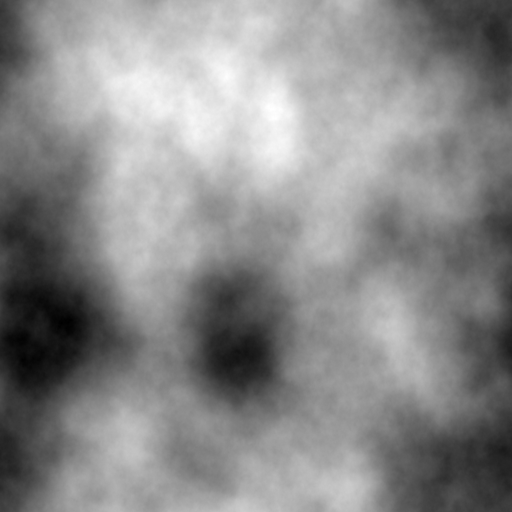
\includegraphics[scale=0.34]{figures/u_30_500km_heights.png}
 }
 \hfill
 \subtop[$\dpd{\eta(\mvec{x},t)}{x}$]
 {
 \label{sfig:derivative_x}
 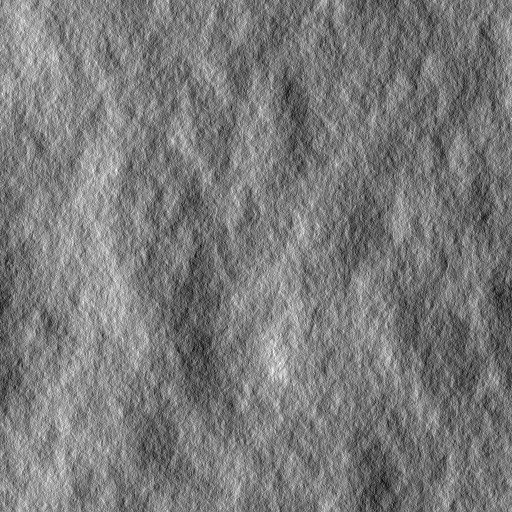
\includegraphics[scale=0.34]{figures/u_30_500km_gradient_x.png}
 }
 \hfill
 \subtop[$\dpd{\eta(\mvec{x},t)}{z}$]
 {
 \label{sfig:derivative_z}
 
\includegraphics[scale=0.34]{figures/u_30_500km_gradient_z.png}
 }
\caption{Brighter means larger values, darker means lower values.
\subcaptionref{sfig:derivative_heights} An example
surface wave height realization, displayed in greyscale (Unified spectrum, 
$U_{10}=30m\cdot s^{-1}$, $F=500km$). \subcaptionref{sfig:derivative_x} The 
first component of the slope vector. \subcaptionref{sfig:derivative_z} The 
second component of the slope vector.
}
\label{fig:derivatives}
\end{figure}
%
Now we may go back to the two-dimensional case, with our original two-dimensional
domains $\mvec{x}$ and $\mvec{k}$. The resolution of said domains is $N \times N$,
the size of the spatial domain is $L \times L$. Let $g(\mvec{k})$ be the
\DiscreteFourierTransform of $f(\mvec{x})$, then we may write the
\InvDiscreteFourierTransform in two dimensions as follows:
\begin{equation*}
 f(\mvec{x}) = \sum_{\mvec{k}}g(\mvec{k})~\mathrm{e}^{\mathrm{i}\transpose{\mvec{k}}\mvec{x}}
\end{equation*}
Based on Equation~\ref{eq:dft_derivative}, and by reusing Equation~\ref{eq:dft_derivative_correction}
because $N$ and $L$ are equal for both dimensions, we find the derivatives of $f(\mvec{x})$:
\begin{equation}
\label{eq:dft_derivates_2d}
 \dmd{f(\mvec{x})}{n+m}{x}{n}{z}{m} = \sum_{\mvec{k}}d(k_{x}, n)d(k_{z}, m)~g(\mvec{k})~\mathrm{e}^{\mathrm{i}\transpose{\mvec{k}}\mvec{x}}
\end{equation}
where $x$ and $z$ denote the two components of vector $\mvec{x}$, and $k_x$ and $k_z$ 
the two components of \wavevector $\mvec{k}$ respectively.
As we need to find the surface slope vector, we need to compute 
the surface elevation's first order partial derivatives. Given surface 
elevation $\eta(\mvec{x},t)$, we obtain the two-dimensional surface slope 
vector $\mvec{s}$ as follows:
\begin{equation}
\label{eq:dft_slope_2d}
 \mvec{s}(\mvec{x},t) = \left[\dpd{\eta(\mvec{x},t)}{x}, \dpd{\eta(\mvec{x},t)}{z}\right]
\end{equation}
We leave it as an exercise for the reader to substitute the terms $\eta(\mvec{x},t)$
and $h(\mvec{k},t)$ into Equation~\ref{eq:dft_derivates_2d} to be able to
compute the surface slope vector as given in Equation~\ref{eq:dft_slope_2d}.
Figure~\ref{fig:derivatives} depicts an example instance of surface 
elevation $\eta$ as well as its associated slopes in greyscale.
%One may notice that Figure~\ref{sfig:derivative_heights}, without prior
%knowledge, is not  recognizable as a wave heightfield. The wave heightfield's
%gradients in Figure~\ref{sfig:derivative_x} and \subcaptionref{sfig:derivative_z},
%on the other hand, are more easily identified as water waves by the human eye.

The two spectra which constitute the surface slope vector in the \wavevector domain
are hermitian. Therefore we are able to apply the optimisation from
Equation~\ref{eq:idft:combined} which allows us to combine both spectra into one,
obtaining both components of the surface slope vector with just one \InvFourierTransform.
%
\subsection{Normal Vectors}
%
In this work we employ a right-handed Carthesian coordinate system where the positive
Y-axis points in the opposite direction of earth's gravity.
The two-dimensional surface slope vector lies in the XZ-plane of the world space
coordinate system. Based on the surface slope vector we may find the unit
length surface normal vector $\mvec{n}$ as follows:
\begin{equation*}
 \mvec{n} = \frac{(-s_x, 1, -s_z)}{\norm{(-s_x, 1, -s_z)}}
\end{equation*}
where $s_x$ and $s_z$ denote the two components of slope vector $\mvec{s}$
as obtained by Equation~\ref{eq:dft_slope_2d}.
%
\subsection{Displacements}
\label{sec:displacements}
%
\begin{figure}
 \centering
 \subtop[$\eta(\mvec{x},t)$]
 {
 \label{sfig:displacement_heights}
 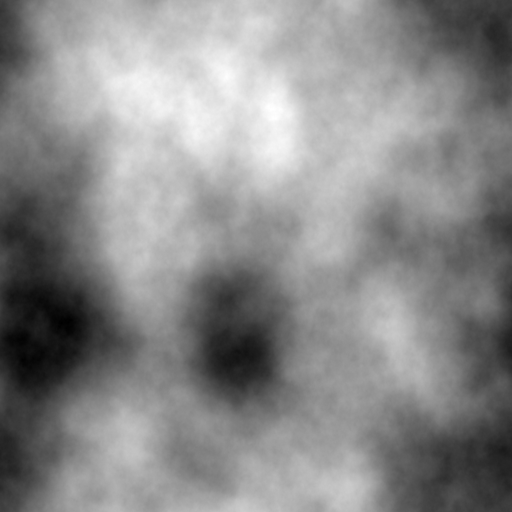
\includegraphics[scale=0.34]{figures/u_30_500km_heights.png}
 }
 \hfill
 \subtop[$D_x(\mvec{x},t)$]
 {
 \label{sfig:displacement_x}
 \includegraphics[scale=0.34]{figures/u_30_500km_displacement_x.png}
 }
 \hfill
 \subtop[$D_z(\mvec{x},t)$]
 {
 \label{sfig:displacement_z}
 \includegraphics[scale=0.34]{figures/u_30_500km_displacement_z.png}
 }
\caption{
Brighter means larger values, darker means lower values.
\subcaptionref{sfig:displacement_heights} An example surface wave height
realization, displayed in greyscale (Unified spectrum, $U_{10}=30m\cdot s^{-1}$, $F=500km$).
\subcaptionref{sfig:displacement_x} The first component of the displacement vector.
\subcaptionref{sfig:displacement_z} The second component of the displacement vector.
}
\label{fig:displacements}
\end{figure}
%
The waves generated with the methods presented up to now tend to have rounded peaks and troughs,
which is typical for fair weather conditions. But we also would like to be able to synthesize waves
matching poor weather conditions, such as strong winds or even storms. During such weather, ocean waves
are sharply peaked at their tops and flattened at the bottoms. \citet{course:simulatingocean}
describes a method based on the \FourierTransform to produce such choppy waves. The concept is simple: displace
the grid points of the spatial domain in the XZ-plane, with the displacement varying locally with the waves.
Note that the displacement is a two-dimensional vector, therefore we end up computing a vector field.
Similar to spectral differentiation, we compute an \InvFourierTransform of the spectrum $h$,
where the latter is modified by an additional term. We may write the displacement vector field as follows:
\begin{equation}
%\label{eq:dft_displacement}
 \mvec{D}(\mvec{x},t) = \left[D_x(\mvec{x},t), D_z(\mvec{x},t)\right]
\end{equation}
with
\begin{align}
\label{eq:displacement_x} D_x(\mvec{x},t) &= \sum_{\mvec{k}}d(k_x, 
k)~h(\mvec{k},t)~\mathrm{e}^{\mathrm{i}\transpose{\mvec{k}}\mvec{x}} \\
\label{eq:displacement_z} D_z(\mvec{x},t) &= \sum_{\mvec{k}}d(k_z, 
k)~h(\mvec{k},t)~\mathrm{e}^{\mathrm{i}\transpose{\mvec{k}}\mvec{x}} \\
%\label{eq:dft_displacement_correction}
 d(l, k) &= \begin{cases}
             0 &\text{if $N$ even, and $k = 0$ or $\abs{l} = 
\frac{N}{2}\frac{2\pi}{L}$,} \\
             -\mathrm{i}\frac{l}{k} &\text{else.}
            \end{cases}
\end{align}
where the term $d(l, k)$, in addition to make sure the resulting spectrum is 
hermitian, also avoids a division by zero at $k = 0$. 
Figure~\ref{fig:displacements} shows an example instance of surface elevation 
$\eta$ as well as its associated displacements in greyscale.
Because the spectra on the righthand side of Equations~\ref{eq:displacement_x} 
and~\ref{eq:displacement_z} are hermitian, we are again able to apply 
Equation~\ref{eq:idft:combined} and obtain both components of the displacement 
vector field with just one \InvFourierTransform.

% The grid points of the spatial domain are two-dimensional, $\mvec{x} = [x_x, 
% x_y]$, and lie in the XZ-plane of our three dimensional space. Embedded into 
% three dimensional space, they represent the ocean plane at rest, $\mvec{p} = 
% [x_x, 0, x_y]$. We may add surface elevation $\eta$ $[x_x, \eta(\mvec{x},t), 
% x_y]$

Given grid point $\mvec{x} = (x,z)$, time $t$ and surface elevation $\eta(\mvec{x},t)$, 
we may write the corresponding three dimensional, vertically displaced vertex 
coordinate as follows:
\begin{equation}
 \mvec{v}(\mvec{x},t) = \begin{bmatrix}x\\ \eta(\mvec{x},t)\\ z\end{bmatrix} 
\end{equation}
With displacement vector $\mvec{D}(\mvec{x},t)$ at hand, according to 
\citet{course:simulatingocean} we may compute the three dimensional,
vertically and horizontally displaced vertex coordinate as follows:
\begin{equation}
\label{eq:displacement_gridpoints}
 \mvec{w}(\mvec{x},t) =
 \begin{bmatrix}
  x + u D_x(\mvec{x},t)\\ 
  \eta(\mvec{x},t)\\
  z + u D_z(\mvec{x},t)
 \end{bmatrix}
\end{equation}
where $u\in\mathbb{R}$ is a user-controlled parameter to scale the importance of the
displacement vector. We have found that the above formula is correct as long as
$u \leq 0$, otherwise the effect is the opposite of what we want to achieve.
Looking at Equation~\ref{eq:displacement_gridpoints},
one can see that it is not the wave heights that are altered, but instead the grid
points on the XZ-plane are transformed based on the spatial structure of the
height field. This particular transformation accomplishes the effects we sought:
the waves' peaks are sharpened and the waves' valleys are broadened.
%
\begin{figure}
\centering
\begin{tikzpicture}
\begin{axis}[
	width=\textwidth,
	height=4cm,
    legend style={draw=none},
    %legend/.append style={nodes={right}},
	legend pos= south west,
	legend cell align=left,
	xtick = {-50, -40, -30, -20, -10, 0, 10, 20, 30, 40, 50},
	ytick = {-0.5, 0, 0.5},
    xlabel={Spatial domain coordinate~$x$~(\si{\metre})},
    ylabel={Surface height~$\eta$~(\si{\metre})},
	%enlarge y limits = 0.2,
]
\addplot[
    color=red,
    solid,
	]
    table [
		col sep=comma, 
		x expr=\thisrowno{0},
		y expr=\thisrowno{2},
	]
	{figures/u_30_500km_x_dx_h.dat};
\addlegendentry{$x$}
\addplot[
    color=blue,
    solid,
	]
    table [
		col sep=comma, 
		x expr=\thisrowno{0} - 3*\thisrowno{1},
		y expr=\thisrowno{2},
	]
	{figures/u_30_500km_x_dx_h.dat};
\addlegendentry{$x + u D_x(x,t)$}
\end{axis}
\end{tikzpicture}
\caption{Red: the original wave profile. Blue: the displaced wave profile, note 
the steep tops and the flattened valleys ($u = -3$).}
\label{fig:grid_displaced}
\end{figure}
%
Figure~\ref{fig:grid_displaced} shows two profiles of the wave height along one 
direction, where one profile uses displaced coordinates, while the other does 
not.
%
\subsection{Slopes after Displacement}
%
Based on Figure~\ref{fig:grid_displaced} one may see that the application 
of displacements does not only alter the underlying grid points, but as a 
direct consequence the surface's slopes, too. Hence, we need to adjust our 
computation of the slope vector to the new circumstances. Given surface 
elevation $\eta(\mvec{x},t)$, displacement vector $\mvec{D}(\mvec{x},t)$,
and grid point transformation $\mvec{x} + u\mvec{D}(\mvec{x},t)$,
according to \citet[private communication]{article:whitecaps} we obtain the
two-dimensional surface slope $\mvec{s}$ as follows:
\begin{equation}
\mvec{s}(\mvec{x},t) = \left[\frac{\dpd{\eta(\mvec{x},t)}{x}}{1 + u 
\dpd{D_x(\mvec{x},t)}{x}}, \frac{\dpd{\eta(\mvec{x},t)}{z}}{1 + u 
\dpd{D_z(\mvec{x},t)}{z}}\right]
\end{equation}
where $u$ is the displacement scale parameter. Now, in addition
to surface height $\eta$, displacement vector $\mvec{D}$, and the slopes of $\eta$,
we also need to compute a partial derivative of $D_x$ and $D_z$ each.
Again, we may compute the latter two by means of spectral
differentiation, see Equation~\ref{eq:dft_derivates_2d}. Morever, we are again
able to apply the optimisation from Equation~\ref{eq:idft:combined} which allows
us to transform the spectra of the two partial derivatives as one.
%
\subsection{Self-Intersections}
\label{sec:self_intersections}
%
\begin{figure}
\centering
\begin{tikzpicture}[
	spy using outlines={circle, magnification=5, connect spies}
]
\begin{axis}[
	width=\textwidth,
	height=4cm,
    legend style={draw=none},
    %legend/.append style={nodes={right}},
	legend pos= south west,
	legend cell align=left,
	xtick = {-50, -40, -30, -20, -10, 0, 10, 20, 30, 40, 50},
	ytick = {-0.5, 0, 0.5},
    xlabel={Spatial domain coordinate~$x$~($\text{m}$)},
    ylabel={Surface height~$\eta$~($\text{m}$)},
	axis lines = left,
	%enlarge y limits = 0.3,
]
\addplot[
    color=red!15!white,
    solid,
	forget plot
	]
    table [
		col sep=comma, 
		x expr=\thisrowno{0},
		y expr=\thisrowno{2},
	]
	{figures/u_30_500km_x_dx_h.dat};
%\addlegendentry{$x$}
\addplot[
    color=blue,
    solid,
	]
    table [
		col sep=comma, 
		x expr=\thisrowno{0} - 7.5*\thisrowno{1},
		y expr=\thisrowno{2},
	]
	{figures/u_30_500km_x_dx_h.dat};
\addlegendentry{$x + u D_x(x,t)$}
\coordinate (spypoint1) at (axis cs:-44,0.45);
\coordinate (magnifyglass1) at (axis cs:-44,2);

\coordinate (spypoint2) at (axis cs:-16,0);
\coordinate (magnifyglass2) at (axis cs:-16,2);

\coordinate (spypoint3) at (axis cs:5.5,-0.425);
\coordinate (magnifyglass3) at (axis cs:5.5,2);

\coordinate (spypoint4) at (axis cs:48.25,0.7);
\coordinate (magnifyglass4) at (axis cs:48.25,2);

\end{axis}
\spy [black, size=2cm] on (spypoint1) in node[fill=white] at (magnifyglass1);
\spy [black, size=2cm] on (spypoint2) in node[fill=white] at (magnifyglass2);
\spy [black, size=2cm] on (spypoint3) in node[fill=white] at (magnifyglass3);
\spy [black, size=2cm] on (spypoint4) in node[fill=white] at (magnifyglass4);
\end{tikzpicture}
\caption{
Background: the original wave profile.
Foreground: the displaced wave profile, with some of the self-intersections
highlighted. We chose a large displacement scaling parameter ($u=-7.5$) to
better emphasize the effect of self-intersection.
%The wave profile from Figure~\ref{fig:grid_displaced}, but with 
%displacement scaling parameter $u=-7.5$ to better emphasize the effect of 
%self-intersection. The non-displaced wave profile is shown in the background.
}
\label{fig:grid_displaced_self_intersection}
\end{figure}
%
The method by \citet{course:simulatingocean} we use to generate 
choppy waves is not devoid of drawbacks.
As shown in Figure~\ref{fig:grid_displaced_self_intersection}, some of the
displacement vectors we compute may be large enough to cause the displaced
geometry to self-intersect. Near the top of some 
waves the surface actually passes through itself, and as a consequence inverts, 
with the surface normal pointing inwards instead of outwards. We may get rid of 
this undesired side-effect in a rather simple way: reduce the magnitude of 
displacement scaling parameter $u$.
On the other hand, \citeauthor{course:simulatingocean} suggests that we use
said self-intersections to our advantage, because they may be able to signal
the breaking of waves, as well as the production of foam and spray. Hence, we
need to be able to test for such self-intersections in an efficient manner.
\citeauthor{course:simulatingocean} recommends to 
compute the determinant of the~\emph{Jacobian matrix} of the transformation 
from grid point $\mvec{x}$ to displaced grid point 
$\mvec{x}+u\mvec{D}(\mvec{x},t)$. Based on the determinant we may decide if 
self-intersection is taking place.
%
%
\begin{figure}
\centering
\begin{tikzpicture}
\begin{axis}[
  width=\textwidth,
  height=10cm,
  legend style={draw=none},
  %legend/.append style={nodes={right}},
  legend pos= south west,
  legend cell align=left,
  xtick = {-50, -40, -30, -20, -10, 0, 10, 20, 30, 40, 50},
  %ytick = {-0.5, 0, 0.5},
  xlabel={Spatial domain coordinate~$x$~($\text{m}$)},
  ylabel={Surface height~$\eta$~($\text{m}$)},
  axis lines = left,
  %enlarge y limits = 0.3,
]
\addplot[
  color=ForestGreen,
  dotted,
  ]
  table [
    col sep=comma, 
    x expr=\thisrowno{0} - 7.5*\thisrowno{1},
    y expr=(1-7.5*\thisrowno{3})*(1-7.5*\thisrowno{6}) - 
    ((-7.5*\thisrowno{5}) * (-7.5*\thisrowno{4})),
  ]
  {figures/u_30_500km_x_dx_h_dxx_dxz_dzx_dzz.dat};
%\addplot[
  %color=red!15!white,
  %solid,
  %forget plot
  %]
  %table [
    %col sep=comma, 
    %x expr=\thisrowno{0},
    %y expr=\thisrowno{2},
    %]
  %{figures/u_30_500km_x_dx_h_dxx_dxz_dzx_dzz.dat};
%\addlegendentry{$x$}
\addplot[
  color=blue,
  solid,
  ]
  table [
    col sep=comma, 
    x expr=\thisrowno{0} - 7.5*\thisrowno{1},
    y expr=\thisrowno{2},
    ]
  {figures/u_30_500km_x_dx_h_dxx_dxz_dzx_dzz.dat};
%\addlegendentry{$x + u D_x(x,t)$}
\addplot[
  color=black,
  solid,
  ]
  table [
    col sep=comma, 
    x expr=\thisrowno{0},
    y expr=0,
    ]
  {figures/u_30_500km_x_dx_h_dxx_dxz_dzx_dzz.dat};
%\addlegendentry{$x + u D_x(x,t)$}
\end{axis}
\end{tikzpicture}
\caption{Blue: the displaced wave profile ($u = -7.5$). Green: the Jacobian 
determinant. Note, that each instance of surface self-intersection is 
accompanied by negative Jacobian determinants.}
\label{fig:grid_displaced_j}
\end{figure}
%
First, we need the Jacobian matrix of the grid point transformation 
$\mvec{g}(\mvec{x},t)=\mvec{x}+u\mvec{D}(\mvec{x},t)$. The Jacobian matrix is 
the matrix of all first order partial derivatives of a vector valued function. 
As grid point transformation $\mvec{g}$ maps from $\mathbb{R}^2$ to 
$\mathbb{R}^2$, the Jacobian matrix is $2\times 2$ in size. Let $\mvec{J}$ be 
the Jacobian matrix of transformation $\mvec{g}$, then we may write:
%
\begin{equation*}
 \label{eq:jacobian_of_displacement}
 \mvec{J}(\mvec{x},t) =
 \begin{bmatrix}
 J_{xx} & J_{xz} \\
 J_{zx} & J_{zz}
 \end{bmatrix}
 =
 \begin{bmatrix}
   1 + u\dpd{D_x(\mvec{x},t)}{x} & u\dpd{D_x(\mvec{x},t)}{z} \\[1em]
   u\dpd{D_z(\mvec{x},t)}{x} & 1 + u\dpd{D_z(\mvec{x},t)}{z}
 \end{bmatrix}
\end{equation*}
Next, we compute the determinant of the Jacobian matrix:
\begin{equation*}
 det(\mvec{J}(\mvec{x},t)) = J_{xx}J_{zz}-J_{zx}J_{xz}
\end{equation*}
%
If the Jacobian determinant at $\mvec{x}$ is positive, then $\mvec{g}$ 
preserves orientation near $\mvec{x}$. If it is negative, $\mvec{g}$ reverses 
orientation. We are interested in the latter case, because wherever the 
surface self-intersects, it actually folds back on itself via a loop, and a 
loop requires a reversal of orientation. Figure~\ref{fig:grid_displaced_j} 
depicts a displaced surface, as well as the corresponding Jacobian 
determinants. One can see that wherever the surface self-intersects, the 
Jacobian determinant is negative.

% \begin{tabular}{lS[table-format = 3]S[table-format = 3.2]}
% \toprule
%   \textbf{Bus} & \multicolumn{2}{c}{\textbf{Bus Load (MVA)}} \\
%                & {Real} & {Complex} \\
%   \midrule
%   b1 &  50 &  30.99 \\
%   b2 & 170 & 105.35 \\
%   b3 & 200 & 123.94 \\
%   b4 & 150 &  49.58 \\
%   \bottomrule
% \end{tabular}

\section{Level of Detail}
\label{sec:level_of_detail}
The core of our ocean model are the spectra discussed in 
Section~\ref{sec:wave_spectra}. We sample the spectra in 
frequency space to obtain vertical and horizontal displacements produced by 
ocean waves. Because the sampling process is done by means of a \DiscreteFourierTransform,
the resulting data can be seamlessly tiled on the ocean surface. 
However, tiling a single perturbation pattern either leads to repetitive 
artifacts if the tile's footprint in world space is small, or to lack of detail 
if the tile's footprint in world space is large. We chose to tackle these 
issues like \citet{misc:oceanlightingfft} and \citet{article:whitecaps},
which compute not only one perturbation pattern, but a set of perturbation
patterns of different size, which are then superimposed over each other.
%, where each pattern is different in size and therefore may sample
%a different part of the spectrum.
Although this approach is not able to entirely remove the tiling artifacts from
the wave field, it is still able to reduce periodicity to the least common
multiple of the pattern periods.
Moreover, as the \wavenumber ranges of the different patterns complement each
other, we are able to extend the sum of waves to include shorter wavelengths,
even as far as into the gravity-capillary wave domain.
%each pattern samples a different part of the spectrum, we are able
%to extend the sum of waves to include shorter wavelengths, even as far as into
%the gravity-capillary wave domain.
Thus, given a sufficient number of patterns,
we may be able to consistently reproduce small-scale detail for closeups of the
water surface.
In practice, up to four different perturbation patterns may suffice to obtain
satisfactory results \citep{article:whitecaps}.

Since we position this work in the context of real-time rendering,
we need to make sure that the accumulated cost of pattern data synthesis
does not prevent us to keep real-time framerates. 
Thus, we may extend the level-of-detail approach by \citet{misc:oceanlightingfft} and
\citet{article:whitecaps} with a multi-resolution scheme, where specific pattern
datasets, such as surface elevation and displacements, are generated at a lower
resolution than the other datasets. 
%Consequentially, the potential reduction of computational workload is exclusively
%dependent on the actual difference between the two resolutions.
%We may conclude that, based on the number of patterns and the resolution(s) of pattern data,
%we are able to strike a well-adjusted balance between model detail and computational workload.

%Second, we reduce the amount of spectral data to transform. We achieve the
%latter by improving upon the level-of-detail approach by \citet{misc:oceanlightingfft}
%and \citet{article:whitecaps} with a multi-resolution scheme, where surface
%elevation and displacements are generated at a lower resolution
%than their respective first-order derivates.

In the remainder of this section we upgrade our equations to handle more than
one perturbation pattern, we explain how to parametrize the different pattern
periods to be able to reduce tiling artifacts as well as reproduce as much
detail as possible, and last we discuss our multi-resolution approach.
%
\subsection{Equations}
At this point, one perturbation pattern consists of surface
elevation $\eta$, displacement vector $\mvec{D}$, the slopes of $\eta$,
and the first order partial derivatives of $\mvec{D}$.
Because we compute the surface
displacements as a sum of waves, it is straightforward to extend our
computations to incorporate not just one perturbation pattern, but a set of
patterns. Let $l \in \mathbb{N}^+$ represent the number of different patterns,
then we may compute the combined surface elevation as follows:
\begin{equation}
 y(\mvec{x},t) = \sum\limits_{i=0}^{l-1}\eta_i(\mvec{x},t)
\end{equation}
In lockstep with the above we compute the slope of the combined surface elevation:
\begin{equation}
 \mvec{s}(\mvec{x},t) = \left[\dpd{y(\mvec{x},t)}{x},\dpd{y(\mvec{x},t)}{z}\right]
 = \left[\sum\limits_i \dpd{\eta_i(\mvec{x},t)}{x}, \sum\limits_i \dpd{\eta_i(\mvec{x},t)}{z}\right]
\end{equation}
Furthermore, we may extend the horizontal grid point transformation required by
the choppy wave algorithm to the following:
\begin{equation}
\mvec{g}(\mvec{x},t) = \mvec{x}+\sum\limits_{i=0}^{l-1}u_i\mvec{D}_i(\mvec{x},t) 
\end{equation}
Thus, we may write the slope of the combined displaced surface elevation as follows:
\begin{equation}
\mvec{s}(\mvec{x},t) = \left[\frac{\sum\limits_i \dpd{\eta_i(\mvec{x},t)}{x}}{1 
+ \sum\limits_i u_i \dpd{D_{xi}(\mvec{x},t)}{x}}, \frac{\sum\limits_i 
\dpd{\eta_i(\mvec{x},t)}{z}}{1 + \sum\limits_i 
u_i\dpd{D_{zi}(\mvec{x},t)}{z}}\right]
\end{equation}
Given the new grid point transformation, we are in need of the corresponding
Jacobian matrix to be able to locate surface self-intersections. We may write:
\begin{equation}
\label{eq:jacobian_of_displacement_multi}
 \mvec{J}(\mvec{x},t) =
 \begin{bmatrix}
 J_{xx} & J_{xz} \\
 J_{zx} & J_{zz}
 \end{bmatrix}
 =
 \begin{bmatrix}
   1 + \sum\limits_i u_i\dpd{D_{xi}(\mvec{x},t)}{x} & \sum\limits_i u_i\dpd{D_{xi}(\mvec{x},t)}{z} \\[1em]
   \sum\limits_i u_i\dpd{D_{zi}(\mvec{x},t)}{x} & 1 + \sum\limits_i u_i\dpd{D_{zi}(\mvec{x},t)}{z}
 \end{bmatrix}
\end{equation}
%
One can see that in case the number of patterns equals one, the new equations
simply fall back to the original ones.
%
\subsection{Tiling}
As mentioned before, we aim to reduce tiling artifacts as much as possible
by superimposing a set of patterns of different size \citep{misc:oceanlightingfft}.
To be able to do so we require a minimum of two patterns: a large one which defines
the general shape of the ocean surface, and a small one for closeup detail.
\citet{Bridson:2015} argues that if one takes such an approach to reduce
periodicity, then it would be best for the different pattern sizes to be related
to each other by an irrational number, because only then one may be able to
generate an aperiodic signal. In short, given pattern size $L$, then we may
obtain the next tile size as $\alpha L$, where $\alpha$ is an irrational number.
\citeauthor{Bridson:2015} goes even further, and states that it would
be best to choose scaling factor $\alpha$ based on the~\emph{golden ratio}
$\varphi = (1 + \sqrt{5})/2$.
Thus, we devised a simple automatism where the user specifies the size of the
largest pattern, and then each subsequent pattern is automatically shrunk in
size by factor $f$, with $f \in \{\varphi^{-1}, 1 - \varphi^{-1}\}$. The two
choices for $f$ represent the lengths of the line segments one obtains if a
line of length one is split in two based on the golden ratio.
Let $L$ be the size of the largest pattern, then we may compute sizes $L_i$ of
the successive patterns as follows:
\begin{align}
\label{eq:pattern_size_i}
 L_i = f^{i} L && 0 < i < l
\end{align}
where $l$ is the number of patterns.

Although the above gives us an aperiodic signal (not accounting for numerical
accuracy), we are not able to completely eliminate periodicity. In some cases
the human observer is still able to recognize that the underlying dominant
structure, as represented by the largest pattern, appears multiple times.
Still, we have found Equation~\ref{eq:pattern_size_i} to be a surprisingly
simple as well as adequate solution to the issue at hand.
Should one deem it necessary, he or she may always choose pattern
sizes via a different mechanism, based on other irrational numbers, or even by
hand as \citeauthor{article:whitecaps} did.

\subsection{\Wavenumber Range}
%
We employ multiple patterns of different size to reduce tiling artifacts. A
convenient side-effect of such an approach is that the combination of multiple
patterns includes more distinct \wavenumbers into the sum of waves than a single
pattern does. However, before we elaborate on the effect of
multiple patterns on \wavenumber sampling, we may concern ourselves with the
\wavenumbers sampled by a single pattern.
Recall that both, the spatial domain and the \wavevector domain, are defined
entirely by size $L$ and resolution $N$. The minimal, non-zero \wavenumber
representable by the \wavevector domain is $k = 2\pi/L$, it depends only on
size. Moreover, the distance between subsequent
sample points in both dimensions is defined as $\Delta k = 2\pi/L$.
Hence, $\Delta k$ depends only on size. Therefore, by choosing size $L$, we do
not only define the minimal \wavenumber we are able to sample, but also
how densely we are able to sample the spectrum. The largest \wavenumber contained
in the \wavevector domain is $k = \sqrt{2}\pi N/L$. So, given size $L$,
resolution $N$ defines how large the \wavenumbers are allowed to grow, giving us
an upper limit of the \wavenumbers involved in the sum of waves. In short, with
size $L$ and resolution $N$ specified for a pattern, we are able to compute the
pattern's \wavenumber range and sampling density.
%
\begin{figure}
\centering
\begin{tikzpicture}
\begin{groupplot}[
	group style={
		columns=4,
		rows=1,
		xlabels at=edge bottom,
		ylabels at=edge left,
	},
    xlabel={$k_d$},
    ylabel=\empty,
	width=0.3\textwidth,
	axis x line=bottom,
%	ymin = 0,
%	ymax = 0.001,
	]
\nextgroupplot[
	ytick=\empty,
	axis y line=none,
	title = {(a) $L=100m$},
	xmin = 0,
	xmax = 1.4,
	]
\addplot[
  color=red,
  %mark color=blue,
  %mark=halfdiamond*,
  fill,
  fill opacity=0.2,
  ]
  table [
    col sep=comma, 
  ]
  {figures/sampling_res_12_area_100.dat} \closedcycle;
\addplot[
  ycomb,
  color=red,
  ]
  table [
    col sep=comma, 
  ]
  {figures/sampling_res_12_area_100.dat};
\nextgroupplot[
	ytick=\empty,
	axis y line=none,
	title = {(b) $L=50m$},
	xmin = 0,
	xmax = 1.4,
	]
\addplot[
  color=red,
  fill,
  fill opacity=0.2,
  ]
  table [
    col sep=comma, 
  ]
  {figures/sampling_res_12_area_50.dat} \closedcycle;
\addplot[
  ycomb,
  color=red,
  ]
  table [
    col sep=comma, 
  ]
  {figures/sampling_res_12_area_50.dat};
\nextgroupplot[
	ytick=\empty,
	axis y line=none,
	title = {(c) $N=12$},
	xmin = 0,
	xmax = 1.5,
	]
\addplot[
  color=blue,
  fill,
  fill opacity=0.2,
  ]
  table [
    col sep=comma, 
  ]
  {figures/sampling_area_100_res_12.dat} \closedcycle;
\addplot[
  ycomb,
  color=blue,
  ]
  table [
    col sep=comma, 
  ]
  {figures/sampling_area_100_res_12.dat};
\nextgroupplot[
	ytick=\empty,
	axis y line=none,
	title = {(d) $N=24$},
	xmin = 0,
	xmax = 1.5,
	]
\addplot[
  color=blue,
  fill,
  fill opacity=0.2,
  ]
  table [
    col sep=comma, 
  ]
  {figures/sampling_area_100_res_24.dat} \closedcycle;
\addplot[
  ycomb,
  color=blue,
  ]
  table [
    col sep=comma, 
  ]
  {figures/sampling_area_100_res_24.dat};
\end{groupplot}
\end{tikzpicture}
\caption{Red: Equal resolution, $N=12$, different size $L$.
%Both, (a) and (b), consist of the same number of samples.
(a) covers a smaller \wavenumber range
than (b) because the former employs a smaller distance $\Delta k = 2\pi/L$
between consecutive sample points.
Blue: Equal size, $L=\SI{100}{\metre}$, different resolution $N$. The distance between
consecutive sample points is equivalent in (c) and (d). (d) covers a larger
\wavenumber range because it contains more samples than (c).}
\label{fig:sampling_area_vs_res}
\end{figure}
%

Let $k_d$ be a set of distinct \wavenumbers based on parameters $L$ and $N$.
With the \wavenumber set $k_d$ at hand we may sample a one-dimensional
\wavenumber spectrum. Figure~\ref{fig:sampling_area_vs_res} depicts a set of
reconstructions of the same one-dimensional \wavenumber spectrum, where one
can see the effects of size $L$ and resolution $N$ on the \wavenumber set $k_d$,
and thus on the reconstructed spectrum.

%\citet{Bridson:2015} argues that if one wants to reduce periodicity by
%superimposing two tiling patterns with different size, then one should employ
%irrational numbers as scaling factors. In short, given pattern size $L$, then
%we may obtain the next tile size as $\alpha L$, where $\alpha$ is an irrational
%number. \citeauthor{Bridson:2015} goes even further, and states that it would
%be best to choose scaling factor $\alpha$ based on the~\emph{golden ratio}
%$\varphi = (1 + \sqrt{5})/2$.

\subsection{\Wavenumber Sampling}
\begin{figure}[p]
\centering
\begin{tikzpicture}
\begin{groupplot}[
	group style={
		columns=4,
		rows=2,
		%xlabels at=edge bottom,
		xlabels at=all,
		ylabels at=edge left,
	},
    xlabel={$k$},
    ylabel=\empty,
	width=0.3\textwidth,
	axis x line=bottom,
%	ymin = 0,
%	ymax = 0.001,
	]
\nextgroupplot[
	ytick=\empty,
	axis y line=none,
	]
\addplot[
  color=red,
  fill,
  fill opacity=0.2,
  unbounded coords=discard,
  ]
  table [
    col sep=comma, 
  ]
  {figures/sampling_scale_03_lod_1.dat} \closedcycle;
\nextgroupplot[
	ytick=\empty,
	axis y line=none,
	]
\addplot[
  color=blue,
  fill,
  fill opacity=0.2,
  unbounded coords=discard,
  ]
  table [
    col sep=comma, 
  ]
  {figures/sampling_scale_03_lod_2.dat} \closedcycle;
\nextgroupplot[
	ytick=\empty,
	axis y line=none,
	]
\addplot[
  color=green,
  fill,
  fill opacity=0.2,
  unbounded coords=discard,
  ]
  table [
    col sep=comma, 
  ]
  {figures/sampling_scale_03_lod_3.dat} \closedcycle;
\nextgroupplot[
	ytick=\empty,
	axis y line=none,
	]
\addplot[
  color=orange,
  fill,
  fill opacity=0.2,
  unbounded coords=discard,
  ]
  table [
    col sep=comma, 
  ]
  {figures/sampling_scale_03_lod_4.dat} \closedcycle;
\nextgroupplot[
	ytick=\empty,
	axis y line=none,
	]
\addplot[
  color=red,
  fill,
  fill opacity=0.2,
  unbounded coords=discard,
  ]
  table [
    col sep=comma, 
  ]
  {figures/sampling_scale_06_lod_1.dat} \closedcycle;
\nextgroupplot[
	ytick=\empty,
	axis y line=none,
	]
\addplot[
  color=blue,
  fill,
  fill opacity=0.2,
  unbounded coords=discard,
  ]
  table [
    col sep=comma, 
  ]
  {figures/sampling_scale_06_lod_2.dat} \closedcycle;
\nextgroupplot[
	ytick=\empty,
	axis y line=none,
	]
\addplot[
  color=green,
  fill,
  fill opacity=0.2,
  unbounded coords=discard,
  ]
  table [
    col sep=comma, 
  ]
  {figures/sampling_scale_06_lod_3.dat} \closedcycle;
\nextgroupplot[
	ytick=\empty,
	axis y line=none,
	]
\addplot[
  color=orange,
  fill,
  fill opacity=0.2,
  unbounded coords=discard,
  ]
  table [
    col sep=comma, 
  ]
  {figures/sampling_scale_06_lod_4.dat} \closedcycle;
\end{groupplot}
\end{tikzpicture}
\caption{
A one-dimensional \wavenumber spectrum reconstructed at resolution $N = 128$,
with initial pattern size $L = \SI{1750}{\metre}$, and subsequent, reduced
pattern sizes obtained by Equation~\ref{eq:pattern_size_i}.
Top row: pattern sizes are reduced by factor $f=1-\varphi^{-1}$.
Bottom row: pattern sizes are reduced by factor $f = \varphi^{-1}$.
Note the difference in \wavenumber range between top and bottom row.
}
\label{fig:sampling_pattern_size_reduction}
\end{figure}
%
%
\begin{figure}[p]
\centering
\begin{tikzpicture}
\begin{groupplot}[
	group style={
		columns=3,
		rows=2,
		%xlabels at=edge bottom,
		xlabels at=all,
		ylabels at=edge left,
	},
    xlabel={$k$},
    ylabel=\empty,
	width=0.35\textwidth,
	axis x line=bottom,
%	ymin = 0,
%	ymax = 0.001,
	]
\nextgroupplot[
	ytick=\empty,
	axis y line=none,
	]
\addplot[
  color=red,
  fill,
  fill opacity=0.2,
  ]
  table [
    col sep=comma, 
  ]
  {figures/sampling_scale_03_lod_1.dat} \closedcycle;
\addplot[
  color=blue,
  fill,
  fill opacity=0.2,
  ]
  table [
    col sep=comma, 
  ]
  {figures/sampling_scale_03_lod_2_capped.dat} \closedcycle;
\nextgroupplot[
	ytick=\empty,
	axis y line=none,
	]
\addplot[
  color=red,
  fill,
  fill opacity=0.2,
  ]
  table [
    col sep=comma, 
  ]
  {figures/sampling_scale_03_lod_1.dat} \closedcycle;
\addplot[
  color=blue,
  fill,
  fill opacity=0.2,
  ]
  table [
    col sep=comma, 
  ]
  {figures/sampling_scale_03_lod_2_capped.dat} \closedcycle;
\addplot[
  color=green,
  fill,
  fill opacity=0.2,
  ]
  table [
    col sep=comma, 
  ]
  {figures/sampling_scale_03_lod_3_capped.dat} \closedcycle;
\nextgroupplot[
	ytick=\empty,
	axis y line=none,
	]
\addplot[
  color=red,
  fill,
  fill opacity=0.2,
  ]
  table [
    col sep=comma, 
  ]
  {figures/sampling_scale_03_lod_1.dat} \closedcycle;
\addplot[
  color=blue,
  fill,
  fill opacity=0.2,
  ]
  table [
    col sep=comma, 
  ]
  {figures/sampling_scale_03_lod_2_capped.dat} \closedcycle;
\addplot[
  color=green,
  fill,
  fill opacity=0.2,
  ]
  table [
    col sep=comma, 
  ]
  {figures/sampling_scale_03_lod_3_capped.dat} \closedcycle;
\addplot[
  color=orange,
  fill,
  fill opacity=0.2,
  ]
  table [
    col sep=comma, 
  ]
  {figures/sampling_scale_03_lod_4_capped.dat} \closedcycle;
\nextgroupplot[
	ytick=\empty,
	axis y line=none,
	]
\addplot[
  color=red,
  fill,
  fill opacity=0.2,
  ]
  table [
    col sep=comma, 
  ]
  {figures/sampling_scale_06_lod_1.dat} \closedcycle;
\addplot[
  color=blue,
  fill,
  fill opacity=0.2,
  ]
  table [
    col sep=comma, 
  ]
  {figures/sampling_scale_06_lod_2_capped.dat} \closedcycle;
\nextgroupplot[
	ytick=\empty,
	axis y line=none,
	]
\addplot[
  color=red,
  fill,
  fill opacity=0.2,
  ]
  table [
    col sep=comma, 
  ]
  {figures/sampling_scale_06_lod_1.dat} \closedcycle;
\addplot[
  color=blue,
  fill,
  fill opacity=0.2,
  ]
  table [
    col sep=comma, 
  ]
  {figures/sampling_scale_06_lod_2_capped.dat} \closedcycle;
\addplot[
  color=green,
  fill,
  fill opacity=0.2,
  ]
  table [
    col sep=comma, 
  ]
  {figures/sampling_scale_06_lod_3_capped.dat} \closedcycle;
\nextgroupplot[
	ytick=\empty,
	axis y line=none,
	]
\addplot[
  color=red,
  fill,
  fill opacity=0.2,
  ]
  table [
    col sep=comma, 
  ]
  {figures/sampling_scale_06_lod_1.dat} \closedcycle;
\addplot[
  color=blue,
  fill,
  fill opacity=0.2,
  ]
  table [
    col sep=comma, 
  ]
  {figures/sampling_scale_06_lod_2_capped.dat} \closedcycle;
\addplot[
  color=green,
  fill,
  fill opacity=0.2,
  ]
  table [
    col sep=comma, 
  ]
  {figures/sampling_scale_06_lod_3_capped.dat} \closedcycle;
\addplot[
  color=orange,
  fill,
  fill opacity=0.2,
  ]
  table [
    col sep=comma, 
  ]
  {figures/sampling_scale_06_lod_4_capped.dat} \closedcycle;
\end{groupplot}
\end{tikzpicture}
\caption{
Gradual assembly of the reconstructed spectra from Figure
\ref{fig:sampling_pattern_size_reduction} into one coherent spectrum.
The transition from data from one spectrum to data from the next
spectrum takes place at the maximum \wavenumber of the spectrum with the
smaller \wavenumber range.
}
\label{fig:sampling_pattern_assembly}
\end{figure}
%
For us to generate a believable, as well as visually pleasing ocean surface, we
are required to include into our sum of waves a finite set of distinct
\wavenumbers such that it is representative of the whole energy.
We have seen in Figure~\ref{fig:sampling_area_vs_res} that if we generate only
one pattern, based on size and resolution, we either sparsely sample inside a
large \wavenumber range, or we densely sample inside a small \wavenumber range.
If, on the other hand, we generate multiple patterns of differing size, then
the patterns' \wavenumbers ranges complement each other. Thus, we are able
to sample a significantly larger \wavenumber range at a varying, but reasonable
density. Varying, because the sampling density changes from pattern to pattern
based on pattern size.
The enlarged \wavenumber range may contain short \wavelengths up to, and
including the gravity-capillary wave domain, which represents waves with a
length from one to several centimeters. With such short waves involved in the
sum of waves we have no difficulties to reproduce sufficient detail for
close-ups of the water surface. Still, we need to make sure to set a lower
limit of $\lambda_{min} = \SI{1.73}{\centi\metre}$ for the \wavelengths included
by any of the patterns, because for waves shorter than $\lambda_{min}$ gravity is
replaced by surface tension as the major restoring force, making them
capillary waves. The latter are not modeled correctly by any of the wave
spectra presented in Section~\ref{sec:wave_spectra}, because those wave spectra
concern themselves exclusively with gravity waves.

%Given the enlarged \wavenumber range, we are able to
%include shorter \wavelengths into the sum of waves, allowing us to reproduce
%sufficient detail for close-ups of the water surface.

Figure~\ref{fig:sampling_pattern_size_reduction} shows that the \wavenumber
ranges of the different patterns are partially overlapping,
therefore we need to make sure to sample each \wavenumber only once.
Thus, if the spectrum of one pattern already covers a specific
\wavenumber range, a second spectrum covering parts or the entirety of that same
range, has to be zeroed in the region of overlap. Moreover, it is the spectrum
of the pattern with larger size that should have precedence, as it has higher
sampling density.
Figure~\ref{fig:sampling_pattern_assembly} shows the assembly of the overlapping
spectra from Figure~\ref{fig:sampling_pattern_size_reduction} into one coherent
spectrum. We get the best sampling density, if the transition from data from
one spectrum to data from the next spectrum takes place at the maximum
\wavenumber of the spectrum with the smaller \wavenumber range.
%Care has to be taken not to sample the same part of the spectrum multiple times.
%FIXME: Double negative. Not doing so, would imply including the same \wavenumber(s) multiple times in the
%sum of waves. Thus, if the spectrum of one pattern already covers a specific
%\wavenumber range, a second spectrum covering parts or the entirety of that same
%range, has to be zeroed in the region of overlap.
%Figure~\ref{fig:sampling_pattern_assembly} shows the assembly of the overlapping
%spectra from Figure~\ref{fig:sampling_pattern_size_reduction} into one coherent
%spectrum. The transition from data from one spectrum to data from the next
%spectrum always happens at the maximum \wavenumber of the spectrum with the
%smaller \wavenumber range.
%include a larger number of distinct \wavenumbers into the sum of waves
%compared to a single pattern.
%The
%former results in a poor reconstruction of a larger part of the spectrum, the
%latter in a better reconstruction of a smaller part of the spectrum, but
%possibly missing other relevant parts of the spectrum. 
%Fortunately, we already generate more than one pattern 
%Thus, if we generate more
%than one pattern, then we may be able to sample as many distinct \wavenumbers as
%possible. As explained before, each pattern has its specific \wavenumber range
%based on pattern resolution and pattern size.
%For simplicity's sake our implementation uses the same resolution for a dataset across all patterns.
%

\emph{Note}: The typical profile of a one-dimensional \wavenumber spectrum suggests
that it would be beneficial to employ an adaptive sampling scheme which allows
for tight sampling in the low \wavenumber range, especially near the peak
\wavenumber, and sparse sampling in the high \wavenumber range
\citep{article:frechot2007}. Because we employ a \DiscreteFourierTransform to
compute the sum of waves, we are subject to its constraints. One of
those constraints is that the spacing between successive coordinates is constant,
namely $\Delta k$. Hence, in combination with a \DiscreteFourierTransform, we
are not allowed to employ a sampling scheme where $\Delta k$ changes dependent
on which part of the \wavenumber profile is being sampled.
%
%
%For us to generate a believable, as well as visually pleasing ocean surface, we
%are required to include into our sum of waves a finite set of \wavenumbers such
%that it is representative of the whole energy. If we generate only one pattern,
%based on size and resolution, we either sparsely sample inside a large
%\wavenumber range, or we densely sample inside a small \wavenumber range. The
%former results in a poor reconstruction of a larger part of the spectrum, the
%latter in a better reconstruction of a smaller part of the spectrum, but
%possibly missing other relevant parts of the spectrum. Thus, we generate more
%than one pattern, where the goal is to sample as many distinct
%\wavenumbers as possible.
%
%\subsection{Pattern Sizes}
%%
%We would like to sample the spectrum at as many \wavenumbers as possible,
%therefore we need to minimize overlap of the \wavenumber ranges of different
%patterns. Because our implementation shares the same dataset resolution(s) $N$
%across all patterns, we are forced to focus on pattern size $L$ to reduce
%\wavenumber overlap.
%%In our implementation each dataset shares the same resolution across
%%all patterns, therefore we focus on pattern size to reduce \wavenumber overlap.
%We need at least one large pattern size, to avoid repetitive artifacts as much
%as possible, and one small pattern size for closeup detail.
%\citet{Bridson:2015} argues that if one wants to reduce periodicity by
%superimposing two tiling patterns with different size, then one should employ
%irrational numbers as scaling factors. In short, given pattern size $L$, then
%we may obtain the next tile size as $\alpha L$, where $\alpha$ is an irrational
%number. \citeauthor{Bridson:2015} goes even further, and states that it would
%be best to choose scaling factor $\alpha$ based on the~\emph{golden ratio}
%$\varphi = (1 + \sqrt{5})/2$.
%
%
%In addition, we have to make sure that the different sizes are not integral
%multiples of each other, otherwise the surface may seem repetitive at a smaller
%scale than expected. 
%FIXME: irrational number~\citet{Bridson:2015}
%We chose to tackle both requirements by
%employing multiples based on the golden ratio $\varphi = (1 + \sqrt{5})/2$. The
%user sets the largest desired pattern size, each following pattern size is
%reduced by the same multiplicative factor $f$, where $f \in \{\varphi^{-1},
%1 - \varphi^{-1}\}$.
%
%
%In case we choose $f = 1-\varphi^{-1} \approx 0.382$, the combined patterns
%allow for tight sampling around the spectral peak as well as in the high
%\wavenumber range. Hence, the sum of waves includes both, large wavelengths which
%give the overall surface its shape, and small wavelengths for close-up detail.
%The drawback of this choice are the smaller pattern sizes, which results in
%repetitive artifacts at a smaller scale than expected. In case we choose
%$f = \varphi^{-1} \approx 0.618$, the combined patterns allow for even more
%tight sampling around the spectral peak, but missing most of the energy in the
%high \wavenumber range. Thus, it is the large wavelengths we are able to
%reconstruct, but missing close-up detail. On the other hand, we have less issues
%with repetitive artifacts. The two rows in Figure~\ref{fig:sampling_pattern_size_reduction}
%depict the reconstructions of one and the same spectrum, based on patterns with
%the same resolution $N$, but initial size $L$ reduced by the two different
%factors.
%
\subsection{Multiple Resolutions}
%
%
\begin{figure}[p]
\centering
\begin{tikzpicture}
\begin{groupplot}[
	group style={
		columns=4,
		rows=2,
		%xlabels at=edge bottom,
		xlabels at=all,
		ylabels at=edge left,
	},
    xlabel={$k$},
    ylabel=\empty,
	width=0.3\textwidth,
	axis x line=bottom,
%	ymin = 0,
%	ymax = 0.001,
	]
\nextgroupplot[
	ytick=\empty,
	axis y line=none,
	xmin = 0,
	xmax = 0.46,
	]
\addplot[
  color=red!20!white,
  ]
  table [
    col sep=comma, 
  ]
  {figures/sampling_multires_scale_06_res_128_8_lod_1.dat};
\addplot[
  ycomb,
  color=red,
  ]
  table [
    col sep=comma, 
  ]
  {figures/sampling_multires_scale_06_res_64_8_lod_1.dat};
\addplot[
  color=red,
  %draw=red,
  fill,
  fill opacity=0.2,
  ]
  table [
    col sep=comma, 
  ]
  {figures/sampling_multires_scale_06_res_64_8_lod_1.dat} \closedcycle;
\nextgroupplot[
	ytick=\empty,
	axis y line=none,
	xmin = 0,
	xmax = 0.74,
	]
\addplot[
  color=blue!20!white,
  ]
  table [
    col sep=comma, 
  ]
  {figures/sampling_multires_scale_06_res_128_8_lod_2.dat};
\addplot[
  ycomb,
  color=blue,
  ]
  table [
    col sep=comma, 
  ]
  {figures/sampling_multires_scale_06_res_64_8_lod_2.dat};
\addplot[
  color=blue,
  fill,
  fill opacity=0.2,
  ]
  table [
    col sep=comma, 
  ]
  {figures/sampling_multires_scale_06_res_64_8_lod_2.dat} \closedcycle;
\nextgroupplot[
	ytick=\empty,
	axis y line=none,
	xmin = 0,
	xmax = 1.2,
	]
\addplot[
  color=green!20!white,
  ]
  table [
    col sep=comma, 
  ]
  {figures/sampling_multires_scale_06_res_128_8_lod_3.dat};
\addplot[
  ycomb,
  color=green,
  ]
  table [
    col sep=comma, 
  ]
  {figures/sampling_multires_scale_06_res_64_8_lod_3.dat};
\addplot[
  color=green,
  fill,
  fill opacity=0.2,
  ]
  table [
    col sep=comma, 
  ]
  {figures/sampling_multires_scale_06_res_64_8_lod_3.dat} \closedcycle;
\nextgroupplot[
	ytick=\empty,
	axis y line=none,
	xmin = 0,
	xmax = 1.94,
	]
\addplot[
  color=yellow!20!white,
  ]
  table [
    col sep=comma, 
  ]
  {figures/sampling_multires_scale_06_res_128_8_lod_4.dat};
\addplot[
  ycomb,
  color=yellow,
  ]
  table [
    col sep=comma, 
  ]
  {figures/sampling_multires_scale_06_res_64_8_lod_4.dat};
\addplot[
  color=yellow,
  fill,
  fill opacity=0.2,
  ]
  table [
    col sep=comma, 
  ]
  {figures/sampling_multires_scale_06_res_64_8_lod_4.dat} \closedcycle;
\nextgroupplot[
	ytick=\empty,
	axis y line=none,
	xmin = 0,
	xmax = 0.46,
	]
\addplot[
  color=red,
  fill,
  fill opacity=0.2,
  ]
  table [
    col sep=comma, 
  ]
  {figures/sampling_multires_scale_06_res_128_8_lod_1.dat} \closedcycle;
\addplot[
  ycomb,
  color=red,
  ]
  table [
    col sep=comma, 
  ]
  {figures/sampling_multires_scale_06_res_128_8_lod_1.dat};
\nextgroupplot[
	ytick=\empty,
	axis y line=none,
	xmin = 0,
	xmax = 0.74,
	]
\addplot[
  color=blue,
  fill,
  fill opacity=0.2,
  ]
  table [
    col sep=comma, 
  ]
  {figures/sampling_multires_scale_06_res_128_8_lod_2.dat} \closedcycle;
\addplot[
  ycomb,
  color=blue,
  ]
  table [
    col sep=comma, 
  ]
  {figures/sampling_multires_scale_06_res_128_8_lod_2.dat};
\nextgroupplot[
	ytick=\empty,
	axis y line=none,
	xmin = 0,
	xmax = 1.2,
	]
\addplot[
  color=green,
  fill,
  fill opacity=0.2,
  ]
  table [
    col sep=comma, 
  ]
  {figures/sampling_multires_scale_06_res_128_8_lod_3.dat} \closedcycle;
\addplot[
  ycomb,
  color=green,
  ]
  table [
    col sep=comma, 
  ]
  {figures/sampling_multires_scale_06_res_128_8_lod_3.dat};
\nextgroupplot[
	ytick=\empty,
	axis y line=none,
	xmin = 0,
	xmax = 1.94,
	]
\addplot[
  color=yellow,
  fill,
  fill opacity=0.2,
  ]
  table [
    col sep=comma, 
  ]
  {figures/sampling_multires_scale_06_res_128_8_lod_4.dat} \closedcycle;
\addplot[
  ycomb,
  color=yellow,
  ]
  table [
    col sep=comma, 
  ]
  {figures/sampling_multires_scale_06_res_128_8_lod_4.dat};
\end{groupplot}
\end{tikzpicture}
\caption{A one-dimensional \wavenumber spectrum as reconstructed by multiple
patterns of different size.
Pattern size $L$ shrinks with each consecutive column, it follows that both rows have
matching distances between successive samples. Top row uses resolution $N = 8$,
whereas bottom row uses $N = 16$. One can see that each reconstruction in top
row is a subset of the reconstruction in bottom row.
%Top and bottom row use equal pattern sizes, it follows that both rows have matching distances between
%subsequent samples. Top row employs half the resolution of bottom row, therefore
%each of its reconstructions is equal the left half of the correspondig
%reconstruction in bottom row.
}
\label{fig:sampling_different_resolutions}
\end{figure}
%
%
Recall, that one perturbation pattern consists of surface elevation $\eta$,
displacement vector $\mvec{D}$, the slopes of $\eta$, and the first order
partial derivatives of $\mvec{D}$. Moreover, we have a set of such patterns. The
computational load to synthesize all the cumulated pattern data has proven to be
substantial. To improve upon the status quo, we chose to implement an approach
common in computer graphics: augment low-resolution geometry with high-resolution
surface information to generate detailed lighting. For our specific case, that
means we may synthesize vertical and horizontal displacements at a lower
resolution than the associated derivatives.
%
%
Given pattern size $L$, grid point spacing $\Delta k = 2\pi/L$, pattern
resolutions $N_h,N_l \in \mathbb{N}$ with $N_l < N_h$, then we may define the
two following \wavevector domains:
%
\begin{align}
\mvec{h} = (k_x,k_z)~&\in~\{(\alpha\Delta k,\beta\Delta k)|-\frac{N_h}{2}\leq\alpha<\frac{N_h}{2},-\frac{N_h}{2}<\beta\leq\frac{N_h}{2}\}\\
\mvec{l} = (k_x,k_z)~&\in~\{(\alpha\Delta k,\beta\Delta k)|-\frac{N_l}{2}\leq\alpha<\frac{N_l}{2},-\frac{N_l}{2}<\beta\leq\frac{N_l}{2}\}
\end{align}
where \wavevector domain $\mvec{h}$ is based on the higher resolution $N_h$ and therefore contains
more pairs $(k_x, k_z)$ than \wavevector domain $\mvec{l}$. One may notice that $\mvec{l}$ is a
subset of $\mvec{h}$ as long as both \wavevector domains share the same grid point
spacing, and thus the same underlying pattern size. Because all pairs $(k_x, k_z)$ in $\mvec{l}$ are also to be found
in $\mvec{h}$, it follows that wave energy $\Theta(\mvec{l})$ is a subset of
$\Theta(\mvec{h})$. Hence, there is no need to generate two separate instances
of the wave energy spectrum with differing resolutions.
% As long as the two different wavevector domains are based on
% the same pattern size, $\mvec{l}$ is a subset of $\mvec{h}$, it follows that
% $\Theta(\mvec{l})$ is a subset of $\Theta(\mvec{h})$. In short, 
The low resolution variant of the wave energy spectrum is already embedded inside the
high resolution variant, see Figure~\ref{fig:sampling_different_resolutions}.
The same applies to the surface elevation spectrum $h$ as defined
by Equation~\ref{eq:dft_h_k_t}, as well as to the spectra of all derived datasets.
If the high-resolution spectrum $ds(\mvec{h})$ of any dataset has been computed and stored,
then we may generate a low-resolution spectrum of said dataset simply by extracting
the respective subset $ds(\mvec{l})$ from $ds(\mvec{h})$. However, as stated before,
we are content with a low-resolution variant of surface elevation $\eta$ and
displacement vectors $\mvec{D}$ respectively.

%If we compute $h(\mvec{h},t)$ and store the results,
%then we may generate a low-resolution variant of the surface simply by
%extracting the subset $h(\mvec{l},t)$ from the stored results.
%
%
\begin{figure}[p]
\centering
\begin{tikzpicture}
\begin{groupplot}[
	group style={
		columns=3,
		rows=2,
		%xlabels at=edge bottom,
		xlabels at=all,
		ylabels at=edge left,
	},
    xlabel={$k$},
    ylabel=\empty,
	width=0.375\textwidth,
	axis x line=bottom,
%	ymin = 0,
%	ymax = 0.001,
	]
\nextgroupplot[
	ytick=\empty,
	axis y line=none,
	xmin = 0,
	xmax = 0.74,
	]
\addplot[
  color=red,
  fill,
  fill opacity=0.2,
  ]
  table [
    col sep=comma, 
  ]
  {figures/sampling_multires_scale_06_res_64_8_lod_1_capped.dat} \closedcycle;
\addplot[
  color=blue,
  fill,
  fill opacity=0.2,
  ]
  table [
    col sep=comma, 
  ]
  {figures/sampling_multires_scale_06_res_64_8_lod_2_capped.dat} \closedcycle;
\nextgroupplot[
	ytick=\empty,
	axis y line=none,
	xmin = 0,
	xmax = 1.2,
	]
\addplot[
  color=red,
  fill,
  fill opacity=0.2,
  ]
  table [
    col sep=comma, 
  ]
  {figures/sampling_multires_scale_06_res_64_8_lod_1_capped.dat} \closedcycle;
\addplot[
  color=blue,
  fill,
  fill opacity=0.2,
  ]
  table [
    col sep=comma, 
  ]
  {figures/sampling_multires_scale_06_res_64_8_lod_2_capped.dat} \closedcycle;
\addplot[
  color=green,
  fill,
  fill opacity=0.2,
  ]
  table [
    col sep=comma, 
  ]
  {figures/sampling_multires_scale_06_res_64_8_lod_3_capped.dat} \closedcycle;
\nextgroupplot[
	ytick=\empty,
	axis y line=none,
	xmin = 0,
	xmax = 1.94,
	]
\addplot[
  color=red,
  fill,
  fill opacity=0.2,
  ]
  table [
    col sep=comma, 
  ]
  {figures/sampling_multires_scale_06_res_64_8_lod_1_capped.dat} \closedcycle;
\addplot[
  color=blue,
  fill,
  fill opacity=0.2,
  ]
  table [
    col sep=comma, 
  ]
  {figures/sampling_multires_scale_06_res_64_8_lod_2_capped.dat} \closedcycle;
\addplot[
  color=green,
  fill,
  fill opacity=0.2,
  ]
  table [
    col sep=comma, 
  ]
  {figures/sampling_multires_scale_06_res_64_8_lod_3_capped.dat} \closedcycle;
\addplot[
  color=yellow,
  fill,
  fill opacity=0.2,
  ]
  table [
    col sep=comma, 
  ]
  {figures/sampling_multires_scale_06_res_64_8_lod_4_capped.dat} \closedcycle;
\nextgroupplot[
	ytick=\empty,
	axis y line=none,
	xmin = 0,
	xmax = 0.74,
	]
\addplot[
  color=red,
  fill,
  fill opacity=0.2,
  ]
  table [
    col sep=comma, 
  ]
  {figures/sampling_multires_scale_06_res_128_8_lod_1_capped.dat} \closedcycle;
\addplot[
  color=blue,
  fill,
  fill opacity=0.2,
  ]
  table [
    col sep=comma, 
  ]
  {figures/sampling_multires_scale_06_res_128_8_lod_2_capped.dat} \closedcycle;
\nextgroupplot[
	ytick=\empty,
	axis y line=none,
	xmin = 0,
	xmax = 1.2,
	]
\addplot[
  color=red,
  fill,
  fill opacity=0.2,
  ]
  table [
    col sep=comma, 
  ]
  {figures/sampling_multires_scale_06_res_128_8_lod_1_capped.dat} \closedcycle;
\addplot[
  color=blue,
  fill,
  fill opacity=0.2,
  ]
  table [
    col sep=comma, 
  ]
  {figures/sampling_multires_scale_06_res_128_8_lod_2_capped.dat} \closedcycle;
\addplot[
  color=green,
  fill,
  fill opacity=0.2,
  ]
  table [
    col sep=comma, 
  ]
  {figures/sampling_multires_scale_06_res_128_8_lod_3_capped.dat} \closedcycle;
\nextgroupplot[
	ytick=\empty,
	axis y line=none,
	xmin = 0,
	xmax = 1.94,
	]
\addplot[
  color=red,
  fill,
  fill opacity=0.2,
  ]
  table [
    col sep=comma, 
  ]
  {figures/sampling_multires_scale_06_res_128_8_lod_1_capped.dat} \closedcycle;
\addplot[
  color=blue,
  fill,
  fill opacity=0.2,
  ]
  table [
    col sep=comma, 
  ]
  {figures/sampling_multires_scale_06_res_128_8_lod_2_capped.dat} \closedcycle;
\addplot[
  color=green,
  fill,
  fill opacity=0.2,
  ]
  table [
    col sep=comma, 
  ]
  {figures/sampling_multires_scale_06_res_128_8_lod_3_capped.dat} \closedcycle;
\addplot[
  color=yellow,
  fill,
  fill opacity=0.2,
  ]
  table [
    col sep=comma, 
  ]
  {figures/sampling_multires_scale_06_res_128_8_lod_4_capped.dat} \closedcycle;
\end{groupplot}
\end{tikzpicture}
\caption{Gradual assembly of the reconstructed spectra from Figure
\ref{fig:sampling_different_resolutions} into one coherent spectrum.
Due to the difference in resolution it follows that top row and bottom row
transition between two successive reconstructions at different \wavenumbers.
One can see that the low-resolution variant of the spectrum in top row is still
able to adequately sample the low \wavenumbers which contain most of the energy
of the entire spectrum.
}
\label{fig:sampling_different_resolutions_pattern_assembly}
\end{figure}
%
%
Because of our multi-resolution approach, we now have two sets of
reconstructions of the wave energy spectrum, based on two different
dataset resolutions.
It follows that the two sets of reconstructions are assembled into two
different coherent spectra.
%For each set of reconstructions we still need to assemble
%the overlapping spectral data into one coherent spectrum.
As before, the transition from one reconstruction to the next takes place at
the maximum \wavenumber of the reconstruction with the smaller \wavenumber
range.
In addition, as to be seen in Figure \ref{fig:sampling_different_resolutions_pattern_assembly},
we must take into consideration that the two sets of
spectral data have different \wavenumber ranges, therefore the transitions from
one reconstruction to the next may take place at different \wavenumbers for
each set.

The goal of our multi-resolution approach is to reduce the computational
workload of pattern data synthesis. One can see that the improvement we are
able to achieve is directly dependent upon the reduction in resolution
of the horizontal and vertical displacements. Thus, we seek to make do with
a minimum of data for surface elevation $\eta$ and displacement vectors
$\mvec{D}$, without compromising the visual end result. Chapter~\ref{ch:summary}
will elaborate on the equilibrium we found between resolution and visual
fidelity of the resulting ocean surface.
%
%Recall Equation~\ref{eq:dft_h0_k}, which synthesizes a random ocean surface
%based on a wave spectrum, and Equation~\ref{eq:dft_h_k_t}, which animates said
%surface. Let us compute the two equations for the high-resolution \wavevector
%domain $\mvec{h}$ and store the results. Now, if we would like to generate an
%instance of the same surface at a lower resolution, we need to take the
%following steps:
%\begin{itemize}
%\item Define a \wavevector domain $\mvec{l}$ with a lower resolution than
 %\wavevector domain $\mvec{h}$, but the same underlying size $L$.
%\item Extract subset $h(\mvec{l},t)$ from $h(\mvec{h},t)$.
%\end{itemize}



%based on \wavevector domain $\mvec{k}$. For each \wavevector we compute
%wave energy $\Theta(\mvec{k})$ and generate a pair of standard normal
%distributed random numbers $(\xi_r,\xi_i)$. Now, if we would like to generate
%an instance of the same surface at a lower resolution, we need to take the
%following steps:
%\begin{itemize}
 %\item Define a \wavevector domain $\mvec{l}$ with a lower resolution than
 %\wavevector domain $\mvec{k}$, but the same underlying size $L$.
 %\item Extract subset $\Theta(\mvec{l})$ from $\Theta(\mvec{k})$.
 %\item For each extracted element of $\Theta(\mvec{k})$, also copy its
 %associated random number pair $(\xi_r,\xi_i)$.
%\end{itemize}
%The last step makes sure that each \wavevector is associated with one specific
%pair of random numbers, be it as part of the low resolution surface as well as
%part of the high resolution surface. The random number pair basically defines
%the amplitude associated with a \wavevector. To be able to reproduce the same
%random surface at different resolutions, the pairing between amplitude and
%\wavevector needs to remain the same across resolutions.

\section{Demo Application}
\label{sec:demo_application}
At this point we have all building blocks of our work in place, therefore we
may proceed with a compact overview of our showcasing application which puts
all the constituent parts into a coherent whole. We implemented a compact demo
application on Linux, it is written in Objective-C and employs the
\citet{misc:gnustep} Base Library, where the latter provides container classes
as well as basic algorithms.
For rendering we use the compatibility profile of OpenGL 3.3 \citep{misc:opengl,misc:opengl33},
where the GLFW library~\citep{misc:glfw}
handles the creation of a window with the desired OpenGL context. Moreover,
it is GLFW which gives us the means to handle mouse and keyboard input.

All of the ocean energy spectra presented in this work were, in a first step,
implemented in \citet{misc:matlab}. This allowed for easy analysis,
debugging and visualization. Only in a second step did we integrate the wave
energy spectra into the demo application, making sure the results matched the
ones of the MATLAB version. In addition, we chose to employ the same library for
\FastFourierTransforms as MATLAB, namely \citet{misc:fftw}. FFTW does
not only provide a standard complex-to-complex \DFT, but also a more specialized
complex-to-real \DFT, which has proven to be beneficial for our use case.

The user is given a wide range of control over frequency spectrum generation:
he or she may configure the number of patterns, the resolution of the vertical
and horizontal displacements, the resolution of the first order partial
derivatives, wind velocity $U_{10}$, fetch $F$, size $L$ of the largest pattern,
and scaling factor $f$ for the automatic pattern size reduction.
Moreover, the user may select the wave energy spectrum model, where all
of the spectra presented in Section~\ref{sec:wave_spectra} are available
options.

The application consists of three running threads: the first thread continuously
generates frequency spectra for the desired number of patterns, then hands them
to a second thread which applies the \IDFT on said spectra. The transformed
data, which represents the animated ocean surface, is then given to the main
thread for rendering.
%
\subsubsection{Surface Mesh}
%
\begin{figure}
\centering
\subtop[Classic Grid]
{
\includegraphics[scale=0.75]{figures/ProjectedGrid_UniformWS.pdf}
\label{fig:subfigprojgrid1}
}
\subtop[Projected Grid]
{
\includegraphics[scale=0.75]{figures/ProjectedGrid_UniformSS.pdf}
\label{fig:subfigprojgrid2}
}
\caption{
\subcaptionref{fig:subfigprojgrid1}
A uniform grid in world space, its projection onto the image plane is not
uniformly spaced though.
\subcaptionref{fig:subfigprojgrid2}
A uniform grid on the image plane, its associated world space positions
are not uniformly spaced.
}
\label{fig:dprojectedgrid}
\end{figure}
%
With all the ocean data synthesized, we may proceed to actually visualize it.
First and foremost we need to take care of the mesh representation of the ocean
surface.
We have already seen that the ocean surface requires a meshing scheme which is
able to automatically adapt to highly distinct viewing situations, such as
closeups of the water surface as well as views with the ocean spanning to the
horizon.
Based on these criteria, we chose to employ the projected grid
~\citep{Hinsinger:2002,thesis:johanson}. The projected grid is based on a
simple concept: to achieve a uniform distribution of detail on the image plane,
a uniformly spaced grid is created in post-perspective space, transformed to
world space and projected onto the $y=0$ plane, see
Figure~\ref{fig:dprojectedgrid}.
Thus, we have constant memory consumption, as the resolution of the grid in
screen space is constant, and we have adaptive level of detail, because all
screen space grid points are projected to points inside the view frustum,
independent of the actual viewing situation. After the vertices have been
projected onto the $y=0$ plane, they are displaced vertically and horizontally
by surface elevation $y(\mvec{x},t)$ and displacement $\mvec{D}(\mvec{x},t)$,
respectively. Last, all vertices are projected normally on the screen via the
viewing pipeline.
%
\subsubsection{Ocean Lighting}
%
% \begin{figure}
%  \centering
%  \subtop[Sky]
%  {
%  \includegraphics[scale=0.125]{figures/preetham_1.png}
%  }
%  \subtop[Sky + Solar Disc]
%  {
%  \includegraphics[scale=0.125]{figures/preetham_solar_disk_1.png}
%  }
%  \subtop[Sky + Solar Disc + Irradiance]
%  {
%  \includegraphics[scale=0.125]{figures/preetham_solar_disk_irradiance_1.png}
%  }
%  \subtop
%  {
%  \includegraphics[scale=0.125]{figures/preetham_2.png}
%  }
%  \subtop
%  {
%  \includegraphics[scale=0.125]{figures/preetham_solar_disk_2.png}
%  }
%  \subtop
%  {
%  \includegraphics[scale=0.125]{figures/preetham_solar_disk_irradiance_2.png}
%  }
%  \subtop
%  {
%  \includegraphics[scale=0.125]{figures/preetham_3.png}
%  }
%  \subtop
%  {
%  \includegraphics[scale=0.125]{figures/preetham_solar_disk_3.png}
%  }
%  \subtop
%  {
%  \includegraphics[scale=0.125]{figures/preetham_solar_disk_irradiance_3.png}
%  }
% \caption{Brak.}
% \label{fig:preetham}
% \end{figure}
\begin{figure}
 \centering
 \subtop[$\theta_{sun} = \ang{0}$]
 {
 \includegraphics[scale=0.125]{figures/preetham_sRGB_D65_turbidity_2_thetaSun_0.png}
 }
 \hfill
 \subtop[$\theta_{sun} = \ang{30}$]
 {
 \includegraphics[scale=0.125]{figures/preetham_sRGB_D65_turbidity_2_thetaSun_30.png}
 }
 \hfill
 \subtop[$\theta_{sun} = \ang{60}$]
 {
 \includegraphics[scale=0.125]{figures/preetham_sRGB_D65_turbidity_2_thetaSun_60.png}
 }
 \hfill
 \subtop[$\theta_{sun} = \ang{90}$]
 {
 \includegraphics[scale=0.125]{figures/preetham_sRGB_D65_turbidity_2_thetaSun_90.png}
 }
 \subtop
 {
 \includegraphics[scale=0.125]{figures/preetham_sRGB_D65_turbidity_4_thetaSun_0.png}
 }
 \hfill
 \subtop
 {
 \includegraphics[scale=0.125]{figures/preetham_sRGB_D65_turbidity_4_thetaSun_30.png}
 }
 \hfill
 \subtop
 {
 \includegraphics[scale=0.125]{figures/preetham_sRGB_D65_turbidity_4_thetaSun_60.png}
 }
 \hfill
 \subtop
 {
 \includegraphics[scale=0.125]{figures/preetham_sRGB_D65_turbidity_4_thetaSun_90.png}
 }
 \subtop
 {
 \includegraphics[scale=0.125]{figures/preetham_sRGB_D65_turbidity_6_thetaSun_0.png}
 }
 \hfill
 \subtop
 {
 \includegraphics[scale=0.125]{figures/preetham_sRGB_D65_turbidity_6_thetaSun_30.png}
 }
 \hfill
 \subtop
 {
 \includegraphics[scale=0.125]{figures/preetham_sRGB_D65_turbidity_6_thetaSun_60.png}
 }
 \hfill
 \subtop
 {
 \includegraphics[scale=0.125]{figures/preetham_sRGB_D65_turbidity_6_thetaSun_90.png}
 }
\caption{
Example instances of the Preetham skylight model: the solar zenith angle
$\theta_{sun}$ increases from left to right, turbidity $T$ increases from top
to bottom.
}
\label{fig:preetham}
\end{figure}
%
Now that we have dealt with the ocean surface mesh, we may move on to the next
aspect of ocean surface rendering, namely the illumination of the water surface.
We chose to implement the illumination model introduced by
\citet{article:oceanlighting} for three reasons. First, it gives visually
pleasing as well as convincing results. Second, in step with our work,
it is tailored to the deep water of the open ocean. Third, it has been adapted by
\citet{misc:oceanlightingfft} in such a way, that the wave energy spectrum has
become an integral part of the lighting model itself.

The lighting term for the water surface, as presented by
\citeauthor{article:oceanlighting} consists of three parts:
reflected light from the sun, reflected light from the sky dome, and refracted
light from the water. The latter term describes the fraction of light from
the sun and sky which has entered the water due to refraction, and leaves it
again due to multiple scattering.
%Because we are in deep water,
%\citeauthor{article:oceanlighting} assume that no light which has entered the
%water body is reflected from the sea bed back to the water surface.
To model the sky dome and the sun \citeauthor{article:oceanlighting} employ the
work of \citet{Bruneton:2008}, where the latter compute the interaction of
light and the atmosphere in its entirety. We, on the other hand, chose not to
extend the scope of this thesis any further with such a complex technique, and
therefore opted for the well-established work of \citet{Preetham:1999}, which
is easy to implement and requires no preprocessing steps.
The Preetham skylight model, as presented in \citet[Section 3.1]{Preetham:1999},
takes only two parameters: one, the position of the sun on the hemisphere, and two,
the haziness of the atmosphere i.e. turbidity.
Figure~\ref{fig:preetham} depicts the effect of the two parameters on
the resulting sky dome.
With the skylight taken care of, we may turn towards the sunlight. We assume
the sun to be a directional light source, which is uniform in color and
intensity for the entire scene. \cite[Section 3.2]{Preetham:1999} gives us
intensity and color of the sunlight based on the position of the sun, where
the result is consistent with the corresponding skylight.
%That is, because 
%\citeauthor{article:oceanlighting} employ an approximation of the BRDF presented
%by \citet{Ross:2005}, where said BRDF is specifically tailored to the
%statistical properties of ocean surfaces. And we have seen in
%Section~\ref{sec:random_sea} that the wave spectrum itself is a statistical
%description of the ocean surface, and thus may provide all data the Ross
%BRDF requires.
%
%which has been adapted for wave spectra by
%\cite{misc:oceanlightingfft}. \citeauthor{article:oceanlighting} employ
%an approximation of the BRDF presented by \citet{Ross:2005}, where said BRDF is
%specifically tailored to the statistical properties of ocean surfaces. And since
%the wave spectrum itself represents a statistical description of the ocean surface,
%it fits very well with said BRDF.
%
%in because it gives believable as well as
%visually pleasing results. Moreover, it has not only been adapted to work
%with a wave spectrum \citep{misc:oceanlightingfft}, the wave spectrum itself
%represents an integral part of the illumination model.

%\citet{article:oceanlighting} augment the work of \citeauthor{Hinsinger:2002} in
%various areas, the most prominent improvement being an adaptive lighting scheme.
%The latter is based on a hierarchical representation which combines geometry,
%normals and a BRDF~\citep{Ross:2005}, where the BRDF is specifically tailored to
%the statistical properties of ocean surfaces. Based on distance from the viewer,
%the algorithm transitions seamlessy from lighting computed with geometry and per
%pixel normals to lighting computed based solely on the statistical distribution
%of ocean surface slopes as modeled by the BRDF, see Figure~\ref{fig:bruneton:transitions}.
%To save computation time for vertex positions, wavetrains are filtered according
%to the size of their associated projected grid cell in world space.
%For the gradient computation in the pixel shader there is an additional step,
%where wavetrains are filtered according to the projected size of the current pixel
%in world space. In addition, \citeauthor{article:oceanlighting} show the
%integration of the BRDF by \citeauthor{Ross:2005} into the computation of
%all necessary lighting terms, namely the reflected light from the sun and from
%the skydome, and the refracted light from the water, as seen in
%Figure~\ref{fig:bruneton:lightingterms}.
%
%\citet{misc:oceanlightingfft} combines the adaptive lighting scheme
%from \citet{article:oceanlighting} with an ocean surface synthesized
%from the wave spectrum presented in~\citet{article:Elfouhaily1997}.
%Wave heights, gradients, as well as the horizontal displacements
%required for the choppy wave algorithm by \citet{course:simulatingocean}
%are computed entirely on the GPU. In an additional step,
%\citet{article:whitecaps} add whitecaps to the ocean lighting model,
%see Figure~\ref{fig:dupuy:whitecaps}.
%
%At this point we make a number of assumptions about the interaction of light
%with the ocean surface, which in part are attributed to the fact that we concern
%ourselves exclusively with deep water. First, the water is deep, therefore no
%light is reflected from the bottom of the ocean back to the surface. Second,
%there are no light sources within the water body.
%
%We concern ourselves only with deep water, allowing us to make a number of
%assumptions about the interaction of light with the water body.
%We concern ourselves only with deep water, therefore we may assume no light is
%reflected from the bottom of the ocean to the ocean surface. It follows that
%the only light exiting the ocean surface from within has previously entered the
%water body via refraction, and leaves it due to scattering.
%Deep water, no light reflected from the ground, only scattering allows for refracted light to reach the surface. Therefore, the appearance of deep water depends largely on the part of the
%incoming light that gets reflected. And most of the incoming light consists of
%direct sunlight and sunlight inscattered via the sky. Therefore we are in need
%of a skylight model. We chose to implement the Preetham Skylight model
%\cite{Preetham:1999}.
\subsubsection{Whitecaps}
The ocean lighting scheme by \citet{article:oceanlighting} does not account for
the breaking of waves on the open ocean. Neither the geometric deformations,
nor the changes in reflectance caused by foam and spray, so called
whitecaps, are incorporated in their model. \citet{article:whitecaps},
on the other hand, extend the work of \citet{misc:oceanlightingfft}
to include whitecaps.
Their contribution is an optimized algorithm to compute for each pixel the
coverage caused by whitecaps. Said coverage depends on the amount of self
intersections taking place inside the world space footprint of the pixel on
the ocean surface. With the whitecap coverage at hand,
\citeauthor{article:whitecaps} then proceed to modify the lighting term at each
pixel accordingly.
The aforementioned self intersections are located using the approach by
\citet{course:simulatingocean}, whereas the computation of the whitecap
coverage is based on fast linear prefiltering methods \citep{Bruneton:2012},
allowing it to leverage the hardware accelerated mipmap generator of modern GPUs.

%Their approach is based on the method by
%\citet{course:simulatingocean} to locate self intersections on the ocean
%surface (Section~\ref{sec:self_intersections}). Given the
%location of a self intersection, the reflectance at that surface position may
%be modified to account for foam and spray.
%
%\citeauthor{article:whitecaps} contribute an optimized algorithm to compute
%the whitecap fractional coverage inside a pixel. Said coverage depends on the
%amount of self intersections which take place inside the world space footprint
%of the pixel on the ocean plane. The algorithm is based on fast linear
%prefiltering methods \citep{Bruneton:2012}, allowing it to leverage the
%hardware accelerated mipmap generator on modern GPUs.
%
%We may generate whitecaps whenever the following function gives a result equal
%one:
%\begin{equation}
 %whitecap(\mvec{x},t) = H(\epsilon - det(\mvec{J}(\mvec{x},t)))
%\end{equation}
%where $det(\mvec{J}(\mvec{x},t))$ is the Jacobian determinant of the horizontal
%displacement function $\mvec{y}(\mvec{x},t) = \mvec{x}+u\mvec{D}(\mvec{x},t)$,
%$H$ is the Heaviside function and the variable $\epsilon$ controls the amount of
%breaking. According to Dupuy et al. we may approximate the whitecap fractional
%coverage $W$ inside a pixel as follows:
%\begin{equation}
 %W = \frac{1}{A}\iint\limits_A whitecap(\mvec{x},t)\mathrm{d}\mvec{x}
%\end{equation}
%where $A$ represents the footprint of the pixel on the ocean plane. Dupuy et al.
%contribute an optimized algorithm to compute $W$ per pixel on the GPU. Their
%algorithm is based on fast linear prefiltering methods, allowing it to leverage
%the hardware accelerated mipmap generator on modern GPUs. It requires an
%additional preprocessing step, with the first order partial derivatives of
%displacements $\mvec{D}(\mvec{x},t)$ of all patterns as input. The output
%consists of variables $k_i$ and $k_i^2$ from Equation 7 and 8 in
%\cite{article:whitecaps}, which are used to compute the per-pixel whitecap
%fractional coverage $W$ via Equation 6 in \cite{article:whitecaps}.

% Given the Jacobian determinant $det(\mvec{J}(\mvec{x},t))$ of the horizontal
% displacement function $\mvec{y}(\mvec{x},t) = \mvec{x}+u\mvec{D}(\mvec{x},t)$,
% we may generate whitecaps whenever the following function gives a result equal
% one:
% \begin{equation}
%  whitecap(\mvec{x},t) = H(\epsilon - det(\mvec{J}(\mvec{x},t)))
% \end{equation}
% where $H$ is the Heaviside function and the variable $\epsilon$ controls the
% amount of breaking.

%  Said modification is based on
% the magnitude of the Jacobian determinant $det(\mvec{J}(\mvec{x},t))$ of the
% horizontal displacement $\mvec{x}+u\mvec{D}(\mvec{x},t)$.

\subsubsection{Tonemapping}
Rendering the ocean illuminated by the Preetham sunlight and skylight results
in an image with a high dynamic range. For proper display of the image, we
need to map it to the lower dynamic range of a standard monitor by means of
a tonemapping operator. We chose to employ the global tonemapping operator
by \citet[Equation 4]{Reinhard:2002} because it is straightforward to implement
and works well on the class of images our demo application renders.
As the dynamic range of the image may change from frame to frame, we found it
beneficial to emulate the behavior of the temporal luminance adaptation process
of human vision. For simplicity's sake we chose to use the temporal luminance
adaptation algorithm by \citet[Equations 5, 6, 7, 12]{Krawczyk:2005}, which
gives acceptable results and is easily integrated with the global tonemapping
operator by \citeauthor{Reinhard:2002}.

%\emph{Note}: For the interested reader we may mention that
%\citet[Equation 1]{Reinhard:2002} is incorrect, for the correct
%version see \citet{Reinhard:2002:erratum}.

%Rendering the Preetham sky and the ocean results in an image with a high dynamic range.
%We need to map said image to the lower dynamic range of a standard monitor, by means
%of a tonemapping operator. We chose Reinhard's global tonemapping operator, see
%Equation 4 in \cite{Reinhard:2002}. It is straightforward to implement and
%works well on the class of images the demo application renders.
%
%In a first step we compute the log-average luminance $\bar L_w$ of the input image.
%Note, that Equation 1 in\cite{Reinhard:2002} is incorrect, see\cite{Reinhard:2002:erratum}.
%The correct form to compute the log-average luminance of an image is as follows:
%\begin{equation}
 %\bar L_w = \exp\left(\frac{1}{N}\sum\limits_{x,y}\log(\delta + L_w(x,y))\right)
%\end{equation}
%where $N$ is the number of pixels in the image, $L_w(x,y)$ is the ''world'' luminance
%for pixel $(x,y)$, and $\delta$ is small positive value to avoid the singularity at
%$\log(0)$. The value of $\bar L_w$ serves as an approximation to the~\emph{key} of
%the scene. The key indicates whether a scene appears subjectively light, normal, or
%dark. Next we define what luminance the log-average luminance is mapped to in the
%result image. We may write:
%\begin{equation}
%\label{eq:luminance_scaling_reinhard}
 %L(x,y) = \frac{a}{\bar L_w}L_w(x,y)
%\end{equation}
%where $L(x,y)$ denotes the scaled luminance, and $a$ represents the value
%$\bar L_w$ is mapped to.
%We may call $a$ the key value, because it controls the key of the resulting image.
%According to Reinhard et. al. for a scene with normal key it is desirable to
%map the log-average luminance to the subjective middle brightness of the
%displayed image, hence to $a=0.18$, where $a$ lies in the interval
%$\interval{0}{1}$. Lower values for $a$ result in a more darker image, higher
%values in a more brighter image. It is in the last step that we actually
%compute the luminance for each pixel of the result image:
%\begin{equation}
%\label{eq:reinhard_operator}
 %L_d(x,y) = \frac{L(x,y)\left(1+\frac{L(x,y)}{L^2_{white}}\right)}{1+L(x,y)}
%\end{equation}
%where $L_{white}$ is the smallest luminance that will be mapped to pure white.
%This formulation brings all luminances $L \leq L_{white}$ within displayable
%range, whereas all luminances $L > L_{white}$ will appear as pure white,
%simulating a simple oversaturation effect.
%
%As luminance conditions may change from frame to frame, we would like to emulate
%the behaviour of the temporal luminance adaptation process of human vision. We
%employ the temporal luminance adaptation algorithm by Krawczyk et. al.
%\cite{Krawczyk:2005}, namely Equations 5, 6, 7 on page three, and Equation 12 on
%page 5. In short, we replace the $\bar L_w$ term in Equation\ref{eq:luminance_scaling_reinhard}
%with a filtered value $\bar L_a$. Based on our notation from above, we may write
%$\bar L_a$ as follows:
%\begin{subequations}
%\begin{align}
 %\bar L_a^{new} &= \bar L_a + (\bar L_w - \bar L_a) (1-e^{-\frac{T}{\tau}}) \\
%\intertext{with}
 %\tau &= \sigma(\bar L_w)\tau_{rod} + (1-\sigma(\bar L_w))\tau_{cone} \\
 %\sigma(L) &= \frac{0.04}{0.04 + L}\\
 %\tau_{rod} &= 0.4\text{s} \\
 %\tau_{cone} &= 0.1\text{s}
%\end{align}
%\end{subequations}
%where $T$ denotes the timestep between two frames, and $\tau$ represents the
%speed of the adaptation process. For further details the reader may consult
%Krawczyk et. al.\cite{Krawczyk:2005}.

%The implementation of the overall tonemapping algorithm is simple: first convert
%each source pixel from RGB to CIE xyY, where the luminance component Y acts as
%the pixel's ''world'' luminance $L_w$. Next, we update the luminance component Y
%according to Equation~\ref{eq:reinhard_operator}, and as a last step convert the
%luminance adjusted xyY color back to RGB and store it in the target. The actual
%colorimetric conversion functions we use are documented in \cite{misc:colorconversion}.
%The log-average luminance $\bar L_w$ is computed for each frame by simple means
%directly on the GPU. We employ a render target the same size as the source image,
%where for each pixel of the source image we compute $\log(\delta + L_w(x,y))$ and
%write it to the render target. Next, we generate the mipmap pyramid for our render
 %target. The highest mipmap level is one pixel in size and gives us
%$\frac{1}{N}\sum\log(\delta + L_w(x,y))$. Hence, we are able to get $\bar L_w$ by sampling
%the highest mipmap level of our render target and then applying $\exp$ on the result.
%Given $\bar L_w$ we are also able to compute the adapted log-average luminance $\bar L_a$.

%%%%%%%%%%%%%%%%%%%%%%%%%%%%%%%%%%%%%%%%%
%%%%%%%%%%%%%%%%%%%%%%%%%%%%%%%%%%%%%%%%%

%\chapter{Results}
\label{ch:results}
%
% The scope of this thesis includes the generation, animation and rendering of the
% surface of an open ocean in real-time. We focus our interest on the synthesis of
% animated ocean surface geometry, for which we will adopt a set of models from
% oceanographic research.

The previous chapter discussed in detail the approach we took to synthesize
the animated ocean surface, including, one, a number of optimizations to reduce
the computational workload, and, two, a level of detail mechanism which does
not only give us fine-grained control over model detail, but also allows us to
reduce potential tiling artifacts. Additionally, we gave an overview of our demo
application, which integrates our approach to ocean surface synthesis
with real-time rendering algorithms which have been developed specifically for
the display of the open ocean.
Thus, with our demo application at hand, we may move on to discuss the
actual results we were able to achieve.

The remainder of this chapter is organized as follows:
Section \ref{sec:results:performance} gives a compact overview of the performance
improvements which we were able to attain for the generation of the ocean
surface spectra as well as for the computation of the sum of waves via the
\InvFourierTransform.
Section \ref{sec:results:synthesis} delineates the pitfalls we encountered
in the context of ocean surface synthesis with wave spectra, and what measures
we took to either overcome or sidestep them.
Last, Section \ref{sec:results:fidelity} discusses the level of visual fidelity
we were able to obtain, with focus on the different wave spectra, as well as
our level of detail approach.
% Before we delve into details, one may look at Figure~\ref{fig:results} which
% depicts all componenents which are part of our ocean lighting implementation.
% compare lighting of all spectrum types (same parameters)
%
\section{Performance}
\label{sec:results:performance}
%
% \begin{table}
% \centering
% \begin{tabular}{@{}l*2{S[table-format=1.2]}*2{S[table-format=2.2]}*2{S[table-format=3.2]}@{}}
% \toprule
% Spectrum & \multicolumn{6}{c}{Time [\si{\ms}]}       \\ \midrule
%          & \multicolumn{6}{c}{Resolution} \\ \cmidrule(l){2-7} 
%          & {$32\times32$} & {$64\times64$}  & {$128\times128$}  & {$256\times256$}  & {$512\times512$} & {$1024\times1024$} \\
% \midrule
% \csvreader[late after line=\\,late after last line=\\\bottomrule]{figures/benchmark_H0_i5_5300u.csv}{}{\csvcoli & \csvcoliv & \csvcolv & \csvcolvi & \csvcolvii & \csvcolviii & \csvcolix}
% \end{tabular}
% \caption{Computation times for the static part of the spectrum at various resolutions
% with different underlying wave energy spectra. One can see that at larger resolutions
% we would be unable to synthesize the static part of the spectrum more than a few times
% a second, much less so in case of more than one level of detail.}
% \label{tab:results:h0}
% \end{table}
%
% \begin{table}
% \centering
% \begin{tabular}{@{}l*2{S[table-format=1.2]}*2{S[table-format=2.2]}*2{S[table-format=3.2]}@{}}
% \toprule
% Spectrum & \multicolumn{6}{c}{Time [\si{\ms}]}       \\ \midrule
%          & \multicolumn{6}{c}{Resolution} \\ \cmidrule(l){2-7} 
%          & {$32\times32$} & {$64\times64$}  & {$128\times128$}  & {$256\times256$}  & {$512\times512$} & {$1024\times1024$} \\
% \midrule
% Heights         & 0.0 & 0.0 & 0.0 & 0.0 & 0.0 & 0.0 \\
% + Displacements & 0.0 & 0.0 & 0.0 & 0.0 & 0.0 & 0.0 \\
% + Gradients     & 0.0 & 0.0 & 0.0 & 0.0 & 0.0 & 0.0 \\
% + Displ Deriv   & 0.0 & 0.0 & 0.0 & 0.0 & 0.0 & 0.0 \\
% \bottomrule
% \end{tabular}
% \caption{Computation times for a single pattern at various resolutions, where
% each row adds the spectra of the respective dataset to the pattern. Thus, at
% first we have one pattern with only the height spectrum, and in the final row
% we have one pattern with all nine spectra: one for height, two for displacements,
% two for gradients, and four for displacement derivatives.
% As all datasets share most of the arithmetic, it is the extra stores to memory
% that require the bulk of the additional CPU time.}
% \label{tab:results:all}
% \end{table}
%
We have seen in Section~\ref{sec:spectrum_synthesis} that the underlying
spectrum of the animated ocean surface consists of two parts, a static part
and a time-dependent part.
As long as the \wavevector domain and the wave energy spectrum's parameters do
not change, the static part of the spectrum has to be computed only once for
the entire lifetime of the animated ocean surface.
Moreover, as it is the static part of the spectrum that incorporates the wave
energy spectrum, we are relieved of a significant computational burden.
That is because evaluating the wave energy spectrum for a large set of
\wavevectors has proven to be extensive in terms of computational complexity.
%
\begin{figure}
\centering
%\tikzset{external/force remake}
\pgfplotstableread[col sep = comma]{figures/benchmark_H0_i5_5300u.dat}\mydata
\begin{tikzpicture}[trim axis left]
  \begin{axis}[
%     ybar,
%     bar width = 6pt,
    legend pos = north west,
    xticklabels from table={\mydata}{Resolution},
    xtick=data,
    xlabel={Resolution [\si{\pixel}]},
    ylabel={Time [\si{\ms}]},
    legend style={draw=none},
    every axis legend/.append style={nodes={right}},
    ]
    \addplot [color=blue] table[x expr=\coordindex, y index = {1}]{\mydata};
    \addplot [color=green!70!black] table[x expr=\coordindex, y index = {2}]{\mydata};
    \addplot [color=black] table[x expr=\coordindex, y index = {3}]{\mydata};
    \addplot [color=red] table[x expr=\coordindex, y index = {4}]{\mydata};

    \addplot[color=black,dashed] coordinates {
    (0,200)
    (4,200)
    }
    node[below,pos=0.5] {$5$ fps};
    \addplot[color=black,dotted] coordinates {
    (0,400)
    (4,400)
    }
    node[below,pos=0.5] {$2.5$ fps};

    % assemble legend
    \pgfplotstablegetcolsof{\mydata}
    \pgfmathparse{\pgfplotsretval-1}
    \foreach \n in {1,...,\pgfmathresult} {
      \pgfplotstablegetcolumnnamebyindex{\n}\of{\mydata}\to{\colname}
      \addlegendentryexpanded{\colname}
    }
  \end{axis}
\end{tikzpicture}
\caption[Computation times for the static part of the spectrum at various
resolutions with different underlying wave energy spectra.]{
Computation times for the static part of the spectrum at various
resolutions with different underlying wave energy spectra.
One can see that at higher resolutions we would be unable to synthesize the
static part of the spectrum more than a few times a second, much less so if we
would employ more than one ocean surface pattern.
Moreover, one may notice that the computation times of the different wave
energy spectra diverge significantly. That is expected, considering
the difference in complexity of the wave energy models in question.
}
\label{fig:results:h0}
\end{figure}
%
See Figure~\ref{fig:results:h0}, which gives an overview of measurements we
have taken for the computation time of the static part of the spectrum for a
single ocean surface pattern.

With the static part of the spectrum on hand in a precomputed form, we are able
to compute the spectra of all datasets within a fraction of time so short that
we may synthesize at least one animated ocean surface pattern in real-time on
a single CPU thread.
%
%
\begin{figure}
\centering
% \tikzset{external/force remake}
\pgfplotstableread[col sep = comma]{figures/benchmark_H_i5_5300u.dat}\mydata
\begin{tikzpicture}[trim axis left]
  \begin{axis}[
    legend pos = north west,
    stack plots = y,
    area style,
    xticklabels from table={\mydata}{Resolution},
    xtick=data,
    xlabel={Resolution [\si{\pixel}]},
    ylabel={Time [\si{\ms}]},
    legend style={draw=none},
    every axis legend/.append style={nodes={right}},
    ]
    \addplot [color=black,fill=black,fill opacity=0.25] table [x expr=\coordindex,y=Heights] from \mydata \closedcycle; 
    \addplot [color=red,fill=red,fill opacity=0.25] table [x expr=\coordindex,y=Slopes] from \mydata \closedcycle;
    \addplot [color=green,fill=green,fill opacity=0.25] table [x expr=\coordindex,y=Displacements] from \mydata \closedcycle;
    \addplot [color=blue,fill=blue,fill opacity=0.25] table [x expr=\coordindex,y=Displacement Derivatives] from \mydata \closedcycle;
    
    \addplot[color=black,dashed,stack plots=false] coordinates {
      (0,20)
      (4,20)
      }
      node[below,pos=0.5] {$50$ fps};
    \addplot[color=black,dotted,stack plots=false] coordinates {
      (0,40)
      (4,40)
      }
    node[below,pos=0.5] {$25$ fps};
%     assemble legend
    \pgfplotstablegetcolsof{\mydata}
    \pgfmathparse{\pgfplotsretval-1}
    \foreach \n in {1,...,\pgfmathresult} {
      \pgfplotstablegetcolumnnamebyindex{\n}\of{\mydata}\to{\colname}
      \addlegendentryexpanded{\colname}
    }
  \end{axis}
\end{tikzpicture}
\caption[Accumulated computation times for the generation of spectral datasets at
various resolutions for a single ocean surface pattern.]{
Accumulated computation times for the generation of spectral datasets at
various resolutions for a single ocean surface pattern.
We start at the bottom with the computation times we measured for the height
spectrum, and step by step add the timings of the remaining datasets.
One can see that the height spectrum alone takes the better
part of the entire computation time.
That is because all datasets share most of the arithmetic operations.
The bulk of the CPU time spent on the supplemental datasets is caused by the
additional stores to memory.
Moreover, one can see that for all resolutions in question, except the highest
one, we are able to generate all spectral datasets of the ocean surface pattern
in real-time.}
\label{fig:results:h}
\end{figure}
%
%
Figure~\ref{fig:results:h} gives an overview of the measurements we have taken
for the accumulated computation time of all spectral datasets for a single
ocean surface pattern. Based on said measurements, one can see that, depending
on pattern resolution, there may be computational resources left at our
disposal.
We may employ those resources to generate additional ocean surface patterns,
i.e., levels of detail.
%
\begin{figure}
\centering
% \tikzset{external/force remake}
\pgfplotstableread[col sep = comma]{figures/benchmark_lods_h_g_d_dd_i5_5300u.dat}\mydata
\begin{tikzpicture}
  \begin{axis}[
    legend pos = north west,
    stack plots = y,
    area style,
    xticklabels from table={\mydata}{Resolution},
    xtick=data,
    xlabel={Resolution [\si{\pixel}]},
    ylabel={Time [\si{\ms}]},
    legend style={draw=none},
    every axis legend/.append style={nodes={right}},
    ]
    \addplot [color=black,fill=black,fill opacity=0.25] table [x expr=\coordindex,y=1] from \mydata \closedcycle; 
    \addplot [color=red,fill=red,fill opacity=0.25] table [x expr=\coordindex,y=2] from \mydata \closedcycle;
    \addplot [color=green,fill=green,fill opacity=0.25] table [x expr=\coordindex,y=3] from \mydata \closedcycle;
    \addplot [color=blue,fill=blue,fill opacity=0.25] table [x expr=\coordindex,y=4] from \mydata \closedcycle;

    \addplot[color=black,dashed,stack plots=false] coordinates {
      (1,20)
      (4,20)
      }
    node[centered,pos=-0.15] {\small{$50$ fps}};
    \addplot[color=black,dotted,stack plots=false] coordinates {
      (1,40)
      (4,40)
      }
    node[centered,pos=-0.15] {\small{$25$ fps}};
%     assemble legend
    \pgfplotstablegetcolsof{\mydata}
    \pgfmathparse{\pgfplotsretval-1}
    \foreach \n in {1,...,\pgfmathresult} {
      \pgfplotstablegetcolumnnamebyindex{\n}\of{\mydata}\to{\colname}
      \addlegendentryexpanded{LOD~\colname}
    }
  \end{axis}
\end{tikzpicture}
\caption[Accumulated computation times for the generation of up to four
ocean surface patterns at various resolutions, where each pattern consists of
all four datasets.]{
Accumulated computation times for the generation of up to four
ocean surface patterns at various resolutions, where each pattern consists of
all four datasets.
For each resolution, the computation times among different LODs diverge only
by a small margin.
One can see that up to a resolution of $256 \times 256$ we are able to generate
four ocean surface patterns at a rate of fifty times per second, whereas at a
resolution of $512 \times 512$ we already have to reduce the number of patterns
to two, and still only reach a rate of twenty-five times per second.}
\label{fig:results:lods}
\end{figure}
%
As all of our ocean surface patterns are self-contained, we may assume
that the computation time to generate $l$ patterns of the same resolution
roughly matches the computation time to generate one pattern, multiplied by
$l$. Figure~\ref{fig:results:lods} corroborates said assumption.
Thus, given the computation time of a single pattern, we may easily estimate
the maximum number of patterns we are able to generate in real-time on a
single CPU thread. Still, we are content with a maximum of four patterns.

Due to performance considerations, we chose the IEEE 754 single-precision
floating-point format \citep{IEEE:754} as the underlying data type for
the implementation of our spectrum generation code. Compared to the
double-precision format, it simultaneously allowed us to cut our memory
requirements in half, as well as accelerate arithmetic operations by taking
advantage of the C99 \citep{C99} math library functions tailored to
single-precision floating point numbers.
%
%\emph{Note}: For our implementation of the spectrum generation code we chose
%to perform all computations in . Thus, compared to double precision, we were able to
%cut our requirements regarding memory in half.
%Besides, take advantage of the C99 \citep{C99} math library functions tailored to
%single-precision floats \citep{loosemore:glibc}
% Initially we were dissatisfied with the resulting estimates, as they were
% correct in telling us that we are unable to generate four fully-fledged ocean
% surface patterns in real-time at a resolution larger than $256 \times 256$.
% Still, that realization has been part of our  motivation to develop the
% multi-resolution approach as presented in Section~\ref{sec:level_of_detail}.
% But it turns out that said approach does very little to ease the computational
% workload for the spectrum generation thread, even though it brings distinct
% performance improvements for both the \FourierTransform thread and the
% rendering thread.
% The underlying cause is twofold. First, the static part of the spectrum is
% required to be available at the largest desired resolution, it follows that the
% necessary memory reads maintain the same access pattern for all spectra,
% independent of their resolution.
% Moreover, as all datasets share most of their arithmetic operations, only a
% small portion of the latter are actually skipped for spectra
% with a lower resolution. Therefore we may conclude that if any non-negligible gain
% in computation time occurs at all, then it is due to the reduced amount of
% stores to memory.
%
% Unfortunately it turns out, that our multi-resolution approach contributes
% only near-negligible improvements when it comes to ocean surface pattern
% generation. As described in Section~\ref{sec:level_of_detail}, the static
% spectrum has to be genereated for the larger of the resolutions of our choosing.
% Moreover, all datasets share most of the arithmetic operations, thus they have
% to be executed for the larger resolution, no savings there. The only real gain
% is a reduction of stores to memory.


%We have seen in Section~\ref{sec:level_of_detail} that all our ocean surface
%patterns are self-contained, 
%
%because each pattern employs a unique
%set of \wavenumbers for the sum of waves. Although \Wavenumber overlap
%we may conclude that the computational cost to generate $l$ patterns of
%the same resolution roughly equals the computational cost to generate one
%pattern, multiplied by $l$. TODO: Explain independence better, each pattern
%stands on its own, all knowledge they reuire to share are the wavenumber ranges,
%and thats only relevant for the static part of the spectrum.

% depending on pattern resolution, we still have computation time at our disposal
\subsubsection{Fourier Transform}
\label{sec:performance:fft}
%
\begin{figure}
\centering
% \tikzset{external/force remake}
\pgfplotstableread[col sep = comma]{figures/benchmark_fftwf_i5_5300u.dat}\fftwf
\pgfplotstableread[col sep = comma]{figures/benchmark_fftw_i5_5300u.dat}\fftw
\begin{tikzpicture}
  \begin{axis}[
    width = 0.75\textwidth,
    ybar,
    xtick pos=left,
    bar width = 6pt,
    legend pos = north west,
    xticklabels from table={\fftw}{Resolution},
    xtick=data,
    xlabel={Resolution [\si{\pixel}]},
    ylabel={Time [\si{\ms}]},
    legend style={draw=none},
    every axis legend/.append style={nodes={right}},
    enlarge y limits = upper,
    %nodes near coords,
    ]
    \addplot [color=red,fill=red]     table[x expr=\coordindex, y expr = \thisrowno{1}*9]{\fftw};
    \addlegendentry{$\text{Double Precision} \times 9$}
%     \addplot [color=green,fill=green]    table[x expr=\coordindex, y expr = \thisrowno{1}*5]{\fftw};
%     \addlegendentry{$\text{Double Precision} \times 5$}
    \addplot [color=black,fill=black]   table[x expr=\coordindex, y expr = \thisrowno{1}*9]{\fftwf};
    \addlegendentry{$\text{Single Precision} \times 9$}
    \addplot [color=blue,fill=blue] table[x expr=\coordindex, y expr = \thisrowno{1}*5]{\fftwf};
    \addlegendentry{$\text{Single Precision} \times 5$}
    
    \draw[dashed] ({rel axis cs:0.025,0}|-{axis cs:0,20}) -- ({rel axis cs:0.975,0}|-{axis cs:0,20}) node[above,pos=0.5] {$50$ fps};
    \draw[dotted] ({rel axis cs:0.025,0}|-{axis cs:0,40}) -- ({rel axis cs:0.975,0}|-{axis cs:0,40}) node[above,pos=0.5] {$25$ fps};
  \end{axis}
\end{tikzpicture}
\caption[Comparison of computation times for the \InvDiscreteFourierTransform
for all nine spectra of a single ocean surface pattern at various resolutions.]{
Comparison of computation times for the \InvDiscreteFourierTransform
for all nine spectra of a single ocean surface pattern at various resolutions.
One can see that the single precision variant of the
\InvDiscreteFourierTransform already reduces the computational workload roughly
by a factor of two compared to the double precision variant. Moreover, if we
transform pairs of hermitian spectra at once, we are able to cut the number
of required \IDFTs from nine to five, further reducing the
computational workload by about forty-five percent.}
\label{fig:idft}
\end{figure}
%
\begin{figure}
\centering
% \tikzset{external/force remake}
\pgfplotstableread[col sep = comma]{figures/benchmark_lods_h_g_d_dd_i5_5300u.dat}\lods
\pgfplotstableread[col sep = comma]{figures/benchmark_fftwf_i5_5300u.dat}\fftwf
\begin{tikzpicture}
  \begin{axis}[
    %set layers,
    ybar stacked,
    xtick pos=left,
    xtick align=outside,
    bar shift = -6pt,
    bar width = 6pt,
    xticklabels from table={\lods}{Resolution},
    xtick=data,
    enlarge y limits = upper,
    enlarge x limits,
    ymin = 0,
    ymax = 260,
    ]
    \addplot [color=violet,fill=violet, forget plot] table[x expr=\coordindex, y=1]{\lods};
    \addplot [color=violet!75!white,fill=violet!75!white, forget plot] table[x expr=\coordindex, y=2]{\lods};
    \addplot [color=violet!50!white,fill=violet!50!white, forget plot] table[x expr=\coordindex, y=3]{\lods};
    \addplot [color=violet!25!white,fill=violet!25!white, forget plot] table[x expr=\coordindex, y=4]{\lods};
  \end{axis}
  \begin{axis}[
    %set layers,
    ybar stacked,
    xtick pos=left,
    xtick align=outside,    
    bar shift = 6pt,
    bar width = 6pt,
    xticklabels from table={\fftwf}{Resolution},
    xtick=data,
    xlabel={Resolution [\si{\pixel}]},
    ylabel={Time [\si{\ms}]},
    legend style={draw=none},
    every axis legend/.append style={nodes={right}, at={(0.05,0.95)}, anchor=north west},
    enlarge y limits = upper,
    enlarge x limits,
    ymin = 0,
    ymax = 260,
    ]
    
    \addplot [color=blue,fill=blue, forget plot] table[x expr=\coordindex, y expr = \thisrowno{1}*5]{\fftwf};
    \addplot [color=blue!75!white,fill=blue!75!white, forget plot] table[x expr=\coordindex, y expr = \thisrowno{1}*5]{\fftwf};
    \addplot [color=blue!50!white,fill=blue!50!white, forget plot] table[x expr=\coordindex, y expr = \thisrowno{1}*5]{\fftwf};
    \addplot [color=blue!25!white,fill=blue!25!white, forget plot] table[x expr=\coordindex, y expr = \thisrowno{1}*5]{\fftwf};
    \addlegendimage{ybar stacked, color=violet, fill=violet} \addlegendentry{Generation}
    \addlegendimage{ybar stacked, color=blue, fill=blue} \addlegendentry{\IDFT}
    
    %\pgfplotsextra{\begin{scope}[on layer=axis foreground]
    \draw[dashed] ({rel axis cs:0.2,0}|-{axis cs:0,20}) -- ({rel axis cs:1,0}|-{axis cs:0,20}) node[centered,pos=-0.1] {\small{$50$ fps}};
    \draw[dotted] ({rel axis cs:0.2,0}|-{axis cs:0,40}) -- ({rel axis cs:1,0}|-{axis cs:0,40}) node[centered,pos=-0.1] {\small{$25$ fps}};    
    %\end{scope}}
  \end{axis}
\end{tikzpicture}
\caption[Accumulated computation times for the generation and transformation
of up to four ocean surface patterns at various resolutions.]{
Accumulated computation times for up to four ocean surface patterns at
various resolutions. For each pattern, all datasets are generated with
single-precision and packed into five spectra. Said spectra are then
transformed with the \IDFT, again with single-precision. One can see that the
generation of the spectra actually takes more time than their transformation
via the \IDFT. Still, up to a resolution of $256 \times 256$ we are
able to keep real-time framerates for both the generation and the transformation
of four ocean surface patterns. Whereas at the next higher resolution,
$512 \times 512$, only the transformation stage is close to real-time
framerates for four patterns.
}
\label{fig:gen:idft}
\end{figure}
%
Recall, that a single ocean surface pattern consists of up to nine spectra:
one for surface elevation $\eta$, two for displacement vector $\mvec{D}$,
two for the slopes of $\eta$, and four for the first order partial derivatives
of $\mvec{D}$.
%Depending on resolution, the computational workload caused by
%nine distinct \InvDiscreteFourierTransforms may already be significant.
%Even more so in case of more than one 
Moreover, we employ up to four distinct ocean surface patterns.
It follows that in the worst case we have to compute the
\InvDiscreteFourierTransform for thirty-six spectra. Depending on pattern
resolution, such a number of \IDFTs may represent a massive computational
burden, especially because all \IDFTs have to be computed for each keyframe
of the animated ocean surface.
Fortunately, all our spectra are hermitian, and as we have seen in
Section~\ref{sec:discrete_fourier_transform}, we may apply the
\InvDiscreteFourierTransform on two hermitian spectra at once.
Therefore the maximum number of required \IDFTs for a single ocean surface
pattern drops from nine to five: two for the displacement derivatives,
one for the displacements, one for the slopes, and one for surface elevation.
It follows that for four distinct ocean surface patterns we have to compute
only twenty \IDFTs instead of the full thirty-six, which represents a decrease
of nearly forty-five percent.

%We did not reproduce the current state of art with regard to the \FourierTransform,
%i.e. compute the \IDFT on the GPU (GPGPU, CUDA, clfft). The reasons are varying,
%but the most compelling is debugging. We have found it difficult to make sure
%that the spectrum is synthesized correctly, because it is essentially gaussian noise,
%thus deviations caused by a faulty implementation still lead to results which hold
%up to casual scrutiny. Thus, keeping all spectrum related computation on the
%CPU side allowed us to assert corretness more easily.
%As we already did a MATLAB implementation and a native one
%in ObjC, an additional one would have expanded the scope of this work unreasonably.
%Still, FFTW does an acceptable job performancewise. Note, that we employed the
%float precision variant of FFTW, since it has proven to provide sufficient
%numerical accuracy for our use case, and outperforms the double precision variant
%by a factor of 1.5.
With the large number of \InvDiscreteFourierTransforms taken care of, we have to
focus on the \IDFT itself to improve performance even further.
As stated earlier in Section~\ref{sec:demo_application}, we employ the FFTW
library~\cite{FFTW05} to compute the \InvDiscreteFourierTransform.
FFTW has support for different floating point
precisions, such as IEEE 754~\citep{IEEE:754} single-precision,
double-precision, as well as quad-precision. Initially we used the
double-precision variant of FFTW, but later on we switched to the
single-precision variant, FFTWF. The reasons are twofold: one, our spectra
are already on hand in single-precision, and two, the
FFTW documentation~\citep{misc:fftw:speed} states that FFTWF outperforms
the double-precision variant roughly by a factor of 1.5.
Moreover, we found that for our specific use case, where all spectra have
power-of-two resolutions, FFTWF consistently outperforms FFTW by an even larger
factor of two. Thus, by switching to single-precision, we are not only able to
double the computational performance of the \IDFT, but also to keep the low
memory requirements of single-precision floating point numbers throughout the
entire process of ocean surface synthesis.

For a compact overview of the performance improvements we have been able to
achieve for the \IDFTs of a single ocean surface pattern, one may look at
Figure~\ref{fig:idft}. It is important to note that said improvements take
effect equally for all the ocean surface patterns we generate, independent of
their number.
Furthermore, one may inspect Figure~\ref{fig:gen:idft}
for a performance comparison between the pattern generation stage and the
\InvDiscreteFourierTransform stage.

%Figure~\ref{fig:idft} gives an overview of the performance improvements
%we have been able to achieve for the \IDFTs of a single ocean surface pattern.
%Figure~\ref{fig:gen:idft}, on the other hand, compares the performance of
%the ocean surface pattern generation stage with that of the
%\InvDiscreteFourierTransform stage, based on up to four distinct patterns.

%Initially we used the standard version of FFTW, which works
%exclusively with floating point numbers in the IEEE 754 double-precision format
%\citep{IEEE:754}.
%But according to FFTW's documentation , the
%single-precision variant of FFTW, in short ~\emph{FFTWF}, outperforms the
%double-precision variant by an overall factor of 1.5. Thus, after careful
%testing, we switched to FFTWF. We found that for our specific use case, where
%all spectra have a power-of-two resolution, FFTWF consistently outperforms
%FFTW roughly by a factor of two. Thus, by switching to FFTWF, we were not only
%able to double performance, but also to reduce the memory requirements of our
%spectra by half.
%\cite{misc:fftw:speed}\cite{misc:cudafft}\cite{misc:clfft}
% Therefore we are able to apply the optimisation from
% Equation~\ref{eq:idft:combined}, which allows us to combine both spectra into one,
% described in Section~\ref{sec:discrete_fourier_transform}\ref{sec:slopes_and_displacements}
%

% \begin{figure}
% \centering
% \tikzset{external/force remake}
% \pgfplotstableread[col sep = comma]{figures/benchmark_lods_h_i5_5300u.dat}\lodsh
% \pgfplotstableread[col sep = comma]{figures/benchmark_lods_h_g_i5_5300u.dat}\lodshg
% \pgfplotstableread[col sep = comma]{figures/benchmark_lods_h_g_d_i5_5300u.dat}\lodshgd
% \pgfplotstableread[col sep = comma]{figures/benchmark_lods_h_g_d_dd_i5_5300u.dat}\lodshgddd
% 
% \begin{tikzpicture}
% \begin{groupplot}[
% 	group style={
% 	  columns=2,
% 	},
% % 	xlabel={\Wavenumber~$k$~(\si{\radian\per\meter})},
% 	width=0.5\textwidth,
% 	%scaled ticks=false,
% 	legend columns=-1,
% 	legend style={/tikz/every even column/.append style={column sep=0.5cm}},
% 	]
% \nextgroupplot[
% %     legend pos = north west,
%     legend to name=grouplegend,
%     stack plots = y,
%     area style,
%     xticklabels from table={\lodsh}{Resolution},
%     xtick=data,
%     xlabel={Resolution [\si{\pixel}]},
%     ylabel={Time [\si{\ms}]},
%     ymax = 295,
%     title = {Heights},
% %     y post scale = 1.5,
% %     legend style={draw=none},
% %     every axis legend/.append style={nodes={right}},
%     ]
%     \addplot [color=black,fill=black,fill opacity=0.25] table [x expr=\coordindex,y=1] from \lodsh \closedcycle; 
%     \addplot [color=red,fill=red,fill opacity=0.25] table [x expr=\coordindex,y=2] from \lodsh \closedcycle;
%     \addplot [color=green,fill=green,fill opacity=0.25] table [x expr=\coordindex,y=3] from \lodsh \closedcycle;
%     \addplot [color=blue,fill=blue,fill opacity=0.25] table [x expr=\coordindex,y=4] from \lodsh \closedcycle;
%     
%     %     assemble legend
%     \pgfplotstablegetcolsof{\lodsh}
%     \pgfmathparse{\pgfplotsretval-1}
%     \foreach \n in {1,...,\pgfmathresult} {
%       \pgfplotstablegetcolumnnamebyindex{\n}\of{\lodsh}\to{\colname}
%       \addlegendentryexpanded{LOD~\colname}
%     }
% \nextgroupplot[
% %     legend pos = north west,
%     stack plots = y,
%     area style,
%     xticklabels from table={\lodshgddd}{Resolution},
%     xtick=data,
%     xlabel={Resolution [\si{\pixel}]},
%     ymax = 295,
%     title = {All Datasets},
% %     y post scale = 1.5,
% %     ylabel={Time [\si{\ms}]},
% %     legend style={draw=none},
% %     every axis legend/.append style={nodes={right}},
%     ]
%     \addplot [color=black,fill=black,fill opacity=0.25] table [x expr=\coordindex,y=1] from \lodshgddd \closedcycle; 
%     \addplot [color=red,fill=red,fill opacity=0.25] table [x expr=\coordindex,y=2] from \lodshgddd \closedcycle;
%     \addplot [color=green,fill=green,fill opacity=0.25] table [x expr=\coordindex,y=3] from \lodshgddd \closedcycle;
%     \addplot [color=blue,fill=blue,fill opacity=0.25] table [x expr=\coordindex,y=4] from \lodshgddd \closedcycle;
% \end{groupplot}
% \node at ($(group c1r1.south)!0.5!(group c2r1.south)$)
% [below,
% yshift=-3\pgfkeysvalueof{/pgfplots/every axis title shift}
% ] 
% {\pgfplotslegendfromname{grouplegend}};
% \end{tikzpicture}
% \caption{KABUMM.}
% \end{figure}



%
% \begin{table}[]
% \centering
% % H generation with quadrant swapping
% % #Lods   8     16    32    64   128   256    512    1024 
% %     1 0.006 0.024 0.080 0.280 1.124  4.511 18.301  75.322 
% %     2 0.009 0.036 0.141 0.581 2.336  9.274 38.325 153.983 
% %     3 0.014 0.054 0.216 0.879 3.523 14.222 58.711 234.903 
% %     4 0.018 0.073 0.294 1.207 4.798 19.733 80.774 319.490
% \begin{tabular}{@{}c*2{S[table-format=1.2]}*2{S[table-format=2.2]}*2{S[table-format=3.2]}@{}}
% \toprule
% \#Lods & \multicolumn{6}{c}{Time [\si{\ms}]}       \\ \midrule
%          & \multicolumn{6}{c}{Resolution} \\ \cmidrule(l){2-7} 
%          & {$32\times32$} & {$64\times64$}  & {$128\times128$}  & {$256\times256$}  & {$512\times512$} & {$1024\times1024$} \\
% \midrule
% 1 & 0.080  & 0.280   & 1.124    &  4.511    & 18.301   &  75.322    \\
% 2 & 0.141  & 0.581   & 2.336    &  9.274    & 38.325   & 153.983    \\
% 3 & 0.216  & 0.879   & 3.523    & 14.222    & 58.711   & 234.903    \\
% 4 & 0.294  & 1.207   & 4.798    & 19.733    & 80.774   & 319.490    \\
% \bottomrule
% \end{tabular}
% \caption{}
% \label{tab:results:h:equal:resolution}
% \end{table}
%
%
%Table~\ref{tab:results:h:equal:resolution} timings for spectrum synthesis
%(geometry, displacements, gradients, displacement derivatives) with
%different number of level of detail. Then a table with FFTW timings.
%Then a H generation table where geometry resolution lower than gradient resolution.
% The static part has to be recomputed only in
% case the \wavevector domain or parameters for the wave energy spectrum change.
% 
% as long parameters do
% not change, the spectrum is static, except for the animation term. Thus, we are
% able to lighten the computational load significantly, because evaluating the
% wave energy at a large number of \wavenumbers is expensive.
% \ref{eq:dft_h0_k}
% \ref{eq:dft_h_k_t_hermitian}
% \ref{sec:discrete_fourier_transform}

% H generation
% #Lods 8 16 32 64 128 256 512 1024 
% 1 0.006 0.024 0.081 0.273 1.095 4.397 17.409 70.361 
% 2 0.008 0.034 0.138 0.566 2.264 9.005 36.332 142.816 
% 3 0.013 0.052 0.213 0.867 3.449 13.660 54.651 220.256 
% 4 0.018 0.071 0.291 1.189 4.707 18.817 75.083 298.944 

% H generation with quadrant swapping
% #Lods 8 16 32 64 128 256 512 1024 
% 1 0.006 0.024 0.080 0.280 1.124 4.511 18.301 75.322 
% 2 0.009 0.036 0.141 0.581 2.336 9.274 38.325 153.983 
% 3 0.014 0.054 0.216 0.879 3.523 14.222 58.711 234.903 
% 4 0.018 0.073 0.294 1.207 4.798 19.733 80.774 319.490

% FFTW
% 8 16 32 64 128 256 512 1024 
% 0.0002 0.0008 0.0036 0.0129 0.0500 0.2640 1.2314 7.0269

%
%Simple \InvFourierTransform vs \InvFourierTransform of two hermitian spectra
%Pattern synthesis at full resolution for all datasets
%Pattern synthesis with our multi-resolution approach
%
\subsection{Multi-Resolution}
% with a multi-resolution scheme, where specific pattern
% datasets, such as surface elevation and displacements, are generated at a lower
% resolution than the other datasets
We have seen in Section~\ref{sec:level_of_detail} that in the context of our
level-of-detail approach we may generate surface elevation $\eta$ and
displacement vector $\mvec{D}$ at a lower resolution than their respective
first order derivatives. We expected the resulting performance gains to be twofold: one,
less data to generate, and two, less data to transform via the \IDFT.
The latter point takes effect as expected, but the former does not.
That is because spectrum generation performance is dominated by a set of
arithmetic operations which are shared by all datasets. As said
arithmetic has to be computed for the datasets with the higher resolution
anyway, the only gain in performance arises from a cutback in memory operations.
We found that said cutback improves spectrum generation performance by at most
ten percent, where the actual improvement is dependent on the difference between
the two resolutions of choice. We must admit, that ten percent are far from
enough to allow us to generate the ocean surface patterns at a significantly
higher rate than before, or at least to use the next-higher resolution for the
derivative datasets. But still, it is a betterment, and the reduced resolution
eases the strain on the subsequent tranformation stage considerably.
% That is
% because the \FastFourierTransform algorithm is $O(n\log{}n)$ \citep{Cooley:1965},
% which means for each time we lower the resolution to the
% next-smaller power-of-two, runtime improves by a factor a bit larger than four.
As one may surmise from Figure~\ref{fig:idft}, at a resolution of $128\times128$
or less, the computation time of a single \IDFT becomes basically negligible.
Thus, in case we employ such a low resolution for surface elevation $\eta$ and
displacements $\mvec{D}$, then we are left with the computation time required
by three \IDFTs instead of five, which represents an improvement of forty percent.
Although such an improvement to the transformation stage does not change
the fact that spectrum generation is the bottleneck of our implementation,
it still frees up resources which may be employed elsewhere.
Furthermore, with two datasets on hand at a lower resolution, we may obtain some
gain in rendering performance because less data needs to be transfered to,
and processed by the GPU.
%\subsection{Conclusions}
%At this point we may give a short summary of our performance work.
%We began with a simple proof-of-concept implementation where we
%were barely able to synthesize a single ocean surface pattern a few times per
%second.
%Given two CPU threads and given that we precompute the static part of the spectrum,
%we are able to generate the spectra of all datasets for four level of details at a
%resolution of $256\times256$ at a rate of about fifty times per second.
%At a resolution of $512\times512$ we may synthesize one level of detail at fifty
%times per second, or two at 25 times per second. Multiresolution approach may improve
%said rates to an extent of ten percent.
%
%In future, generate static part of the spectrum on the CPU, do further steps on the
%GPU, such as generate the spectra for the animated surface and apply \InvDiscreteFourierTransform. 
%
%TODO Summing up: we got performance to the point where we are able to synthesize four
%distinct levels of detail at a resolution of 256 x 256 in real-time with two
%cpu threads. 

% In short, dependening on the choice of lower resolution, we may further improve
% spectrum transformation performance by up to forty percent.
% surface synthesis and rendering.
% the derivative datasets at the next-higher resolution, or to significantly
% improve the rate at which we generate the coean surface patterns.
% Still, given two datasets of lower resolution,
% $\eta$ and $\mvec{D}$, which are packed into two spectra, 
% which still represents an adequate betterment.
% \IDFT performance on the other hand scales linearly, $O(n\log{}n)$
% one for surface elevation $\eta$, two for displacement vector $\mvec{D}$,
% two for the slopes of $\eta$, and four for the first order partial derivatives
% of $\mvec{D}$.
% Little to no performance gain for spectrum generation, way more for \IDFT.
% Indirect profits, because of less upload bandwith to GPU, faster texture sampling
% with reduced resolution.

\emph{Note}: All results of benchmarking shown throughout this section
have been collected on an off-the-shelf laptop running an Intel\textregistered
Core\texttrademark i5-5300U Mobile Processor \citep{intel:5300u}.
All our benchmarking code runs on a single CPU thread and gives the average
computation time after repeating the desired task for several thousand iterations.
%
\section{Ocean Surface Synthesis}
\label{sec:results:synthesis}
%Independent of performance, we encountered two major issues with respect to
%the qualitative aspects of ocean surface synthesis: one, wave geometry is
%inadequate, two, ocean surface lighting is inconsistent across different
%wave spectra.
%TODO Two issues: one with geometry (integral domains), one with lighting (mss).
Now that we have discussed the performance aspects of our approach
to ocean surface synthesis, we may focus on the qualitative aspects.
Recall, that we set out to generate and render a visually pleasing,
as well as believable ocean surface. Performance aside, we had to tackle two
major challenges to reach said goal: one, generate convincing wave geometry, and two, 
render the generated ocean with a lighting algorithm which gives plausible results.
For each of the two tasks we encountered at least one major pitfall, which we will
discuss subsequently.
\subsection{Wave Geometry}
Initially, after having implemented all the wave energy
spectra presented in this work, we were dissatisfied with the results.
There was always something \emph{off} about the resulting ocean surface, more
specifically, there seemed to be a mismatch in scale between the length of the
waves and their respective amplitudes. Neither the geometry nor the animation of
the ocean surface looked believable to the observer. It was even worse if we
applied the choppy-wave algorithm to the ocean surface. Hence, in a first step we
tried to mitigate the issue by introducing several fudge factors which allowed
us, one, to rescale the ocean surface's geometry during rendering, and two,
to directly influence the magnitude of the spectrum's energy output. 
By carefully tuning said fudge factors, we were at least able to obtain
acceptable results. Still, each time we switched to a different wave energy
spectrum or modified any of the parameters involved
in the synthesis of the ocean surface, we had to adapt our fudge factors too.
A most cumbersome and error-prone task for the user.
It was only later on that we found the underlying cause of the issue:
we were missing the proper integral domain conversions for all of our wave energy
spectra. %(Section~\ref{subsec:integral_domain_conversion}).
After implementing said conversions, the issue simply vanished.
%according to Section \ref{subsec:integral_domain_conversion},
We finally got believable, comprehensible as well as consistent results across
all wave energy spectra presented in this work, with the only exception being
the Phillips spectrum. Since the latter does not model the ocean surfaces'
underlying physical processes in an appropriate manner, it
is neither consistent with the other spectra nor does it give acceptable
results without significant tuning of the fudge factors. Thus, we decided to
drop the Phillips spectrum from our implementation, and all of the now unused
fudge factors with it.
% and therefore is unable
%to give results up to par with the wave energy spectra that stem from oceanographic
%research.
%Given that the Phillips spectrum is neither consistent with the other spectra, nor
%does it give acceptable results without significant tuning of the fudge factors,
%we decided to drop it, and all of the fudge factors with it.
%to model the ocean surfaces' underlying physical processes in an appropriate
%manner.
%drop all of the fudge factors as they were not needed anymore. 
%That is because from then on  except
%
%and still obtain not only acceptable results, but
%actually believable ones. Except for \citeauthor{course:simulatingocean}'s
%Phillips spectrum, which in its ad-hoc nature is unable to model the underlying
%physical processes in an appropriate manner (Section \ref{sec:phillips_spectrum}).
\subsection{Ocean Surface Lighting}
\label{sec:results:lighting}
%
\begin{figure}
\centering
\subtop[Pierson-Moskowitz]
{
	\includegraphics[width=0.225\textwidth]{figures/ross_pm_complete.png}
}
\hfill
\subtop[JONSWAP]
{
	\includegraphics[width=0.225\textwidth]{figures/ross_jonswap_complete.png}
}
\hfill
\subtop[Unified]
{
	\includegraphics[width=0.225\textwidth]{figures/ross_unified_complete.png}
}
\hfill
\subtop[Donelan]
{
	\includegraphics[width=0.225\textwidth]{figures/ross_donelan_complete.png}
}
\subtop
{
	\includegraphics[width=0.225\textwidth]{figures/ross_pm.png}
}
\hfill
\subtop
{
	\includegraphics[width=0.225\textwidth]{figures/ross_jonswap.png}
}
\hfill
\subtop
{
	\includegraphics[width=0.225\textwidth]{figures/ross_unified.png}
}
\hfill
\subtop
{
	\includegraphics[width=0.225\textwidth]{figures/ross_donelan.png}
}
\caption[Example rendering of the sun reflectance for each spectrum.]{
Example rendering of the same scene for each of the remaining four spectra
($U_{10}=\SI{10}{\metre\per\second}$, $F=\SI{250}{\km}$).
First row: the ocean surface rendered with the lighting algorithm by
\cite{article:oceanlighting}.
Second row: the respective sun reflectance term.
One can see that the sun reflectance of the Donelan spectrum significantly
exceeds that of the other spectra.
}
\label{fig:sun_reflectance}
\end{figure}
%
\begin{figure}
\centering
\begin{tikzpicture}
\begin{groupplot}[
group style={
	columns=2,
	ylabels at=edge left,
	xlabels at=edge bottom,
	horizontal sep=2.0cm,
},
width=0.475\textwidth,
ylabel = {mss~($\si{\meter\radian}$)},
%scaled ticks=false,
legend columns=-1,
legend style={/tikz/every even column/.append style={column sep=0.1cm}},
]
\nextgroupplot[
xlabel = {Wind Speed~$U_{10}$~(\si{\meter\per\second})},
legend to name=grouplegend,
]
\addplot[
color=blue,
solid,
]
table [col sep=comma]{figures/mss_pm_wind_0_30_fetch_250km.dat};
\addlegendentry{Pierson-Moskowitz}
\addplot[
color=green!70!black,
solid,
]
table [col sep=comma]{figures/mss_jonswap_wind_0_30_fetch_250km.dat};
\addlegendentry{JONSWAP}
\addplot[
color=black,
solid,
]
table [col sep=comma]{figures/mss_donelan_wind_0_30_fetch_250km.dat};
\addlegendentry{Donelan}
\addplot[
color=red,
solid,
]
table [col sep=comma]{figures/mss_unified_wind_0_30_fetch_250km.dat};
\addlegendentry{Unified}

\nextgroupplot[
%ylabel={},
xlabel = {Fetch~$F$~(\si{\km})},
scaled ticks = false,
yticklabel style={/pgf/number format/.cd,fixed,fixed zerofill,precision=2},
every axis x label/.style={
	at={(ticklabel* cs:0.5,15pt)},
	anchor=north,
},
%ytick pos=right,	
]
\addplot[
color=blue,
solid,
]
table [col sep=comma]{figures/mss_pm_fetch_5km_100km_wind_10.dat};
\addplot[
color=green!70!black,
solid,
]
table [col sep=comma]{figures/mss_jonswap_fetch_5km_100km_wind_10.dat};
\addplot[
color=black,
solid,
]
table [col sep=comma]{figures/mss_donelan_fetch_5km_100km_wind_10.dat};
\addplot[
color=red,
solid,
]
table [col sep=comma]{figures/mss_unified_fetch_5km_100km_wind_10.dat};
%\draw [black, dashed] (axis cs:0,0.035) rectangle (axis cs:40,0.05);
\end{groupplot}
\node at ($(group c1r1.north)!0.5!(group c2r1.north)$)
[below,
yshift=3\pgfkeysvalueof{/pgfplots/every axis title shift}
] 
{\pgfplotslegendfromname{grouplegend}};
\end{tikzpicture}
\caption[The total mean square slope over wind speed and fetch.]{
Left: the total mean square slope $mss$ over wind speed $U_{10}$ ($F=\SI{250}{\km}$).
One can see that the Donelan spectrum severely overestimates
the total mean square slope of the ocean surface.
Right: the total mean square slope over fetch $F$ ($U_{10} =\SI{10}{\meter\per\second}$).
%Not only the Donelan spectrum overestimates
%the total mean square slope, under low-fetch conditions the JONSWAP spectrum does
%too, but not by such a large amount.
One can see that under low-fetch conditions the JONSWAP spectrum overestimates the
total mean square slope too, but not by such a large amount as the Donelan spectrum
does.
%One can see that under low fetch conditions
%the JONSWAP spectrum overestimates the total mean square slope too.
}
\label{fig:mss_wind_fetch}
\end{figure}
%
Now that we have dropped the Phillips spectrum, we are left with four wave energy
spectrum models. Although all of them give convincing results geometry-wise,
it is only three of them that work well with the lighting algorithm by
\cite{article:oceanlighting}: the Pierson-Moskowitz spectrum, the JONSWAP
spectrum, and the Unified spectrum. The fourth spectrum, namely the Donelan
spectrum, is not eligible because in combination with \cite{article:oceanlighting}
it results in an ocean surface which reflects too much of the incoming sunlight.
%and therefore does not look believable to the observer.
Figure~\ref{fig:sun_reflectance} depicts an example of said shortcoming.
We found that the underlying cause is that the Donelan spectrum does not give
a good approximation of the ocean surface's actual \emph{mean square slopes}
(Appendix~\ref{app:mss}).
The mean square slopes of the ocean surface represent statistical moments
which describe the distribution of the surface waves' slopes~\citep{Massel:2011},
and as such give a measure of the roughness of the ocean surface.
Moreover, the mean square slopes are an essential component of the
lighting model by \cite{article:oceanlighting}, where they are required for
the computation of the sun reflectance term.

Given the importance of the mean square slopes with respect to the
quality of the visual appearance of the ocean surface, we came to
the conclusion that it would be best to employ only wave energy
spectra which give an as good as possible approximation of the mean
square slopes for the entire parameter space of wind speed $U_{10}$
and fetch $F$.
Figure~\ref{fig:mss_wind_fetch} shows that the Donelan spectrum
unconditionally fails to meet this specific requirement. The JONSWAP
spectrum, on the other hand, tends to overestimate the mean square slopes
only for low-fetch conditions, but not by an amount so large that it
would noticeably compromise the plausibility of the end result.
But still, that leaves only two of the five wave energy models presented
in this work to be unconditionally able to measure up to the challenge,
namely the Pierson-Moskowitz spectrum and the Unified spectrum.

%
%it is only the Pierson-Moskowitz
%spectrum and the Unified spectrum which are able to meet this specific
%requirement.
%Figure~\ref{fig:sun_reflectance} depicts an example where the shortcoming
%of the Donelan spectrum is easy to identify.
%few examples where these three spectra give better results than the Donelan
%spectrum.
%
% where all of them give
%convincing results geometry-wise. But still, it is the Pierson-Moskowitz spectrum and the
%Unified spectrum that give the best results with the lighting algorithm
%by \cite{article:oceanlighting}.
%Figure~\ref{fig:sun_reflectance} depicts a few examples where
%the Donelan spectrum and the JONSWAP spectrum do not give results as good
%as the other two spectra.
%The root cause for the shortcomings of the latter two spectra is that
%both do not give that good an approximation of the ocean surface's
%actual \emph{mean square slopes} (Appendix~\ref{app:mss}).
%
%That is because the JONSWAP
%spectrum and the Donelan spectrum do not give that good an approximation
%of the ocean surface's actual \emph{mean square slopes} (Appendix~\ref{app:mss}).
%The mean square slopes are an essential component of the lighting model by
%\cite{article:oceanlighting}, as they are required for the computation of
%the ocean surface's sun reflectance term.

%Thus it is favorable for the wave spectrum to give a good
%approximation of the mean square slopes for as much of the parameter space
%for wind speed and fetch as possible.

%Figure~\ref{fig:mss_wind_fetch} on the other
%hand shows the different approximations of the total mean square slope
%by the four spectra.

%The mean square slopes are a statistical measure of the ocean surface's
%wave slopes.
%Although all spectrum types give convincing results geometry-wise, it is the
%Preetham spectrum and the Unified spectrum that work best with the lighting
%algorithm by \cite{article:oceanlighting}. Probable cause is that the JONSWAP
%spectrum and the Donelan spectrum give not that good an approximation of the
%ocean surface's mean square slope (\ref{app:mss}).
%The mean square slope is a
%core component of the lighting model by \cite{article:oceanlighting}, and thus
%has large influence on the result.

\section{Visual Fidelity}
\label{sec:results:fidelity}
%
Now that we have taken care of the pitfalls which we encountered during
our work on ocean surface generation, we may focus on the overall visual
quality we were able to achieve.

Let us begin with the most fundamental building block, namely the wave spectrum.
Given any one of the wave energy spectra presented in this work
that stem from oceanographic research, one is able to synthesize an ocean
surface where the shape and the animation of the waves does
not only look plausible, but convincing to the observer.
Thus, the only remaining question left for the user is what
kind of sea does he want to generate, and which spectrum would best
fit his choice. We may give some direction on that matter.
If one has a gentle sea in mind, then it would be best to use the Pierson-Moskowitz spectrum, whereas for highly turbulent seas
one should prefer the JONSWAP spectrum. For all the kinds of sea that reside
between those two extrema, the Unified spectrum is the wave energy model of
choice. Even more so, because of the spectra presented in this work it is the
only one to handle gravity-capillary waves in a sensible manner, and is therefore the one
best suited for closeups where short waves are visible to the observer.
%
%
\begin{figure}
\centering
 \subtop[]
 {
  \includegraphics[width=0.48\textwidth]{figures/20-06-2018_14-49-57_complete.png}
 }
 \hfill
 \subtop[]
 {
  \includegraphics[width=0.48\textwidth]{figures/21-06-2018_10-44-51_complete.png}
 } 
\caption[Overview of results.]{The ocean surface under a variety of conditions.}
\label{fig:results:overview}
\end{figure}
%
%
\begin{figure}
\centering
 \subtop[Projected Grid]
 {
  \includegraphics[width=0.48\textwidth]{figures/28-05-2018_10-56-10_grid.png}
 \label{fig:results:grid}
 }
 \hfill
 \subtop[Sun Contribution]
 {
  \includegraphics[width=0.48\textwidth]{figures/28-05-2018_10-56-10_ross.png}
	\label{fig:results:ross}
 }
 \hfill
 \subtop[Sky Contribution]
 {
  \includegraphics[width=0.48\textwidth]{figures/28-05-2018_10-56-10_sky.png}
	\label{fig:results:sky}
 }
 \hfill
 \subtop[Sea Contribution]
 {
  \includegraphics[width=0.48\textwidth]{figures/28-05-2018_10-56-10_sea.png}
	\label{fig:results:sea}
 }
 \hfill
 \subtop[Whitecaps Contribution]
 {
  \includegraphics[width=0.48\textwidth]{figures/28-05-2018_10-56-10_whitecaps.png}
	\label{fig:results:whitecaps}
 }
 \hfill
 \subtop[Final Result]
 {
  \includegraphics[width=0.48\textwidth]{figures/28-05-2018_10-56-10_complete.png}
	\label{fig:results:complete}
 }
\caption[An overview of the meshing scheme and all ocean lighting terms involved
in our implementation.]{
An overview of the meshing scheme and all ocean lighting terms involved in our
implementation.
\subcaptionref{fig:results:grid} The ocean surface as represented by the projected grid.
\subcaptionref{fig:results:ross} Sun light reflected by the water surface.
\subcaptionref{fig:results:sky} Sky light reflected by the water surface.
\subcaptionref{fig:results:sea} Light refracted from the water body.
\subcaptionref{fig:results:whitecaps} Whitecap foam.
\subcaptionref{fig:results:complete} The final result.
}
\label{fig:results:lighting}
\end{figure}
%
%
\begin{figure}
\centering
\includegraphics[width=\textwidth]{figures/19-06-2018_17-10-50_tiles.png}
\caption[Depiction of ocean surface tiles.]{A top down view of the ocean
overlayed with a simple depiction of its four pattern sizes.}
\label{fig:results:tiling}
\end{figure}
%
%

Now, given the wave spectrum of our choosing, we synthesize all datasets
for the desired number of ocean surface patterns and use them to render
the ocean. We have found that for most viewing conditions two complementary
ocean surface patterns provide sufficient visual quality for the
average observer. For closeups, though, it has proven beneficial to
include at least one additional pattern which adds short wave detail to
the water surface. Also for wide spanning camera views, where the ocean
is visible up to the horizon, we settled not for two, but for three to
four patterns to keep tiling artifacts in check. As for pattern resolution,
we chose $256\times256$ because it is the highest resolution which
still allows us to keep real-time framerates with four active patterns.

Given we are satisfied with the visual appearance of the ocean for a specific
number of patterns, then we may employ our multi-resolution approach
to lighten the computational load of CPU and GPU. By simple visual inspection
we have found that for most scenes we are able to reduce the resolution of
the horizontal and vertical displacements as far as to $32\times32$ without
noticing a significant drop in visual quality, on condition that we keep a
resolution of $256\times256$ for the slopes and the first order derivatives.
%
With surface heights and displacements synthesized at such a low resolution,
the computational cost required by them shrinks to nearly zero, freeing
up resources which we may employ elsewhere.
%
Still, there are cases where the observer may notice a distinct drop in
visual quality: one, in closeups, and two, in scenes with highly turbulent
seas where the low resolution may deny the waves their distinctive narrow
peaks.
%
%But still, with surface heights
%and displacements synthesized at such a low resolution, the computational cost
%required by them shrinks to nearly zero.

Now that we have discussed the factors which have most impact on the visual
fidelity of the result, we may give an overview of the variety of
ocean surfaces which we are able to display by means of this work, see
Figure~\ref{fig:results:overview}.
For a rough breakdown of our approach to ocean surface lighting,
one may look at Figure~\ref{fig:results:lighting},
which shows the actual mesh representation of the ocean, all involved
lighting terms, and the final result.
Figure~\ref{fig:results:tiling}, on the other hand, depicts an example
instance of the ocean surface tiles. 
%At this point we conclude the
%discussion of our results and move on to the next chapter, the summary.

%At last, Figure~\ref{fig:results:overview} gives an overview
%of the variety of ocean surfaces we are able to display by means of this work.

%Figure~\ref{fig:results:lighting} depicts an example where one
%can see the actual mesh representation of the ocean, all involved lighting
%terms, and the final result. Figure~\ref{fig:results:tiling}, on the other
%hand, highlights the ocean's tiling pattern. At last,
%Figure~\ref{fig:results:overview} gives an overview of the variety of
%ocean surfaces we are able to synthesize and render using our approach.

%Now, given the wave geometry of our choosing, we may move on to the actual
%process of rendering the ocean surface.
%We have seen that for rendering, wave geometry alone is not sufficient.
%Figure~\ref{fig:results}
%Thus, given all four datasets 
%Given wave geometry data (elevation adn displacements) and its associated datasets
%(slopes and derivatives)


%The Unified spectrum covers the
%remaining ground between those two variants, but is neither able to reach
%the degree of calmness of the Pierson-Moskowitz spectrum nor the overly
%agitated state of the JONSWAP spectrum at low fetch. That makes the Unified
%spectrum the spectrum of choice for most situations, especially because it
%is the one that gives the best results for closeups, as it is the only model
%to handle short waves in a sensible manner.
%
%The latter two follow the general rule, where the general rule
%is, the lower the fetch the more agitated the sea becomes.
%On the geometry side we are satisfied with the results, as both the waves
%themselves and their animation look believable to the observer.
%For wave geometry it is the Pierson-Moskowitz spectrum which
%gives the most calm sea, whereas the JONSWAP spectrum results in a
%more rough and turbulent sea. The Unified spectrum is able to bridge
%those two variants, but never reaching the degree of calmness of the Pierson-Moskowitz spectrum. Also for closeups it is the Unified spectrum which gives the best results, as it is the only model to handle really short waves well.

 
%Regarding our multi-resolution approach to level of detail we have seen that we are able to reduce the resolution of the horizontal
%and vertical displacements as far as to $32\times32$ without
%noticing a large drop in visual quality, as long as we keep a
%resolution of $128\times128$ or higher for the slopes and first
%order derivatives.
%
%Morevoer, it is obvious that the whitecaps algorithm takes a huge
%toll on both CPU and GPU side, four spectra at high resolution,
%which then need all to be sampled per pixel to compute the
%whitecpas coverage. Maybe use another, more simpler approach altogether.
%
%Lets discuss our overall results
%Images of all partial terms involved in ocean lighting (specular by sun,
%reflection of sky, refracted light, whitecaps)
%Image of ocean geometry (wireframe)
%
%Troubles with reflection vectors below horizon
%Troubles with bright patches caused by reflection
%Troubles with dark patches caused by reflection
%Troubles with sundisk (XYZ to sRGB)
%
%Tiling images
%
%Comparison full resolution patterns vs multi-resolution scheme
%
%Maybe different tonemapping settings

%%%%%%%%%%%%%%%%%%%%%%%%%%%%%%%%%%%%%%%%%
%%%%%%%%%%%%%%%%%%%%%%%%%%%%%%%%%%%%%%%%%

%\chapter{Summary}
\label{ch:summary}
%Paste the actual text from the introduction.
%We may approach a more specific subject, namely the synthesis of animated ocean
%surfaces which are both believable and computationally feasible.
%
%The scope of this thesis includes the generation, animation and rendering of the
%surface of an open ocean in real-time. We focus our interest on the synthesis of
%animated ocean surface geometry, for which we will adopt a set of models from
%oceanographic research. Specific properties of said models allow for
%easy addition and reduction of detail, as well as for a range of algorithmic
%optimizations. The former combined with the latter gives us the opportunity to
%strike a well-adjusted balance between model detail and computational workload,
%and thereby to improve upon the status quo of current implementations.
%
We stated in the introduction that in this work we seek to synthesize
animated ocean surfaces which are both believable and computationally feasible.
%We stated in the introduction that in this work we seek to synthesize the open
%ocean in such a manner that it does not only look believable to the observer,
%but is computationally feasible as well.
%
%We stated in the introduction that in this work we seek to generate and render the
%open ocean in real-time. Moreover, we aim for an ocean surface which does not only
%look visually pleasing, but also believable to the observer. Given that context,
%we chose to focus our efforts on wave geometry, because no lighting algorithm
%is able to make good on unrealistic wave shapes.
To achieve said objective, we picked the choppy wave algorithm by \citet{course:simulatingocean},
which adopts the wave spectrum concept from oceanographic research for
computer graphics purposes.
\citeauthor{course:simulatingocean} approximates the
perturbations produced by the water surface by sampling the wave
spectrum in frequency space via the \FastFourierTransform algorithm.
%
%we adopt the wave spectrum concept from
%oceanographic research for computer graphics purposes, as shown in
%\citet{course:simulatingocean}.
%
%The latter approximates the
%perturbations produced by the water surface by sampling the wave
%spectrum in frequency space via the \FastFourierTransform algorithm.
%For the purpose of ocean surface synthesis we opted for the approach by
%\citet{course:simulatingocean}, where the perturbations produced
%by the water surface are approximated by sampling the wave spectrum via
%the \FastFourierTransform algorithm.
The \FFT algorithm is highly efficient and has the additional advantage
of generating a perturbation pattern which seamlessly tiles the ocean surface.
A further upside of the wave spectrum approach is that oceanographic
research includes a wide range of wave spectra which are specifically
tailored to the deep water of the open ocean. Said wave spectra are
employed for oceanographic forecasts and simulations, therefore they
provide a high degree of realism.
Thus, we chose to implement four such wave energy spectra,
%\citep{article:PiersonMoskowitz1964, article:Hasselman1973, article:Donelan1985, article:Elfouhaily1997}, \citep{course:simulatingocean}
all well established in oceanographic literature, plus the wave
spectrum introduced by \citeauthor{course:simulatingocean} (Section~\ref{sec:wave_spectra}).
The latter spectrum was unable to produce results which meet the high
standard given by the other spectra, and therefore we dropped it
(Section \ref{sec:phillips_spectrum} and \ref{sec:results:synthesis}).
The remaining four spectra, on the other hand, allowed us to obtain
animated wave geometry at the level of quality we sought after,
but only after we had made sure that each wave spectrum had been converted
to the correct integral domain (Section~\ref{subsec:integral_domain_conversion}).
%

For the purpose of ocean surface lighting we decided to implement the
algorithm by \citet{misc:oceanlightingfft} as it gives believable results
and it has specifically been tailored to the wave spectrum of the open ocean.
After a successful implementation it turned out that only two of our
remaining wave spectra were able to unconditionally match the algorithms
stringent requirements, with a third spectrum keeping up under most
conditions (Section~\ref{sec:results:lighting}).
Furthermore, we implemented the work by \citet{article:whitecaps} to
incorporate whitecaps into the ocean surface's lighting model.

With ocean surface synthesis and lighting taken care of, we found that
as long as we employ only one perturbation pattern, we may not
be able to reproduce a high-quality ocean surface for all possible
viewing situations. Depending on the observer's viewpoint, we may be
faced with tiling artifacts or lack of detail.
Therefore we adopted the approach by~\citet{misc:oceanlightingfft},
which addresses both matters by superimposing multiple, complementary perturbation
patterns of different size (Section~\ref{sec:level_of_detail}).
With multiple patterns at hand, where for each pattern we have to
generate and Fourier transform up to nine separate spectra (one for vertical
perturbation, two for horizontal perturbation, two for gradients,
four for whitecaps), pattern generation had become computationally too
expensive to still allow for real-time operation.
Therefore we took a number of measures to restore real-time behaviour.
First, we split surface synthesis into two separate threads, where the first
one generates the pattern's actual spectra, and the second one
applies the \InvFourierTransform on said spectra (Section~\ref{sec:demo_application}).
%First, we moved pattern generation as well as 
%and transformation via \FFT to separate threads each (Section~\ref{sec:demo_application}).
Second, as the spectrum consists of a static part and a time-dependent part,
we made sure to compute only the time-dependent part of the spectrum for each
frame (Section~\ref{sec:spectrum_synthesis}).
Third, as all of our spectra are hermitian, we were able to compute the
\InvFourierTransform of two spectra at once (Section~\ref{sec:discrete_fourier_transform}).
%Hence,
%we were able to reduce the maximum number of \InvFourierTransforms per pattern
%from nine to five.
Fourth, we switched the \InvFourierTransform from double precision to single
precision, accelerating its computation by a factor of two
(Section~\ref{sec:performance:fft}).

With performance back to real-time framerates, we improved upon the work by
\citet{misc:oceanlightingfft} with a multi-resolution variant, where
the water surface's wave geometry is synthesized at a lower resolution
than its respective normal vectors and whitecaps
(Section~\ref{sec:implementation:multires}).
The lower resolution lead to a considerable speedup of the \FourierTransform
stage, but not to a significant degradation in visual quality for most scenes
(Section~\ref{sec:results:fidelity}).
%For a large range of distinct scenes the reduced resolution did not seem
%to degrade visual quality in a significant way.
Thus we decided to permanently keep the multi-resolution approach, as it
allows for an even more fine-grained balance between model detail and performance.
%

%Furthermore, we implemented the lighting algorithm by \cite{article:whitecaps},
%which has been specifically tailored to wave spectra.

%
%
%Thus we are given the
%means to further improve performance by 
%
%The latter approach
%allowed us for a more fine-grained balance between model detail and performance. 

%Naturally, multiple patterns imply an increase in computational cost of
%pattern generation. To still be able to generate the ocean surface in
%real-time
%
%With only one perturbation pattern at hand, one may be faced with tiling
%artifacts or lack of detail, depending on the observer's viewpoint.


%First, discretisation and multiple patterns, for proper sampling. Then,
%hermitian spectra to improve performance. Then multi-resolution, again,
%for performance.

%Ocean lighting scheme tailored to the above (Bruneton, Dupuy), another spectrum
%disqualified.

%With our goal being to render the open ocean, we found that discretisation
%of the wave spectrum had proven to be an issue, as we were not sampling enough
%distinct \wavenumbers to reproduce a high-quality ocean surface for all
%possible viewing situations. We addressed the matter by using multiple,
%complementary wave patterns which sample different, non-overlapping parts
%of the wave spectrum. During this work, up to four of such patterns where
%always sufficient.

%but only after we made sure to meet a set of preconditions. First and
%foremost, we had to ensure that each wave spectrum of interest is
%converted to the correct integral domain. Second,  
%
%Wave energy spectrum from oceanographic research provides realistic wave geometry
%and animation, given integral domain conversion is done correctly.
%Discretisation is an issue, addressed by additional levels of detail.
%Simple solution for tiling via sizes with irrational numbers.
%Multi-resolution approach to reduce performance impact of level-of-detail
%algorithm.
%Ocean lighting scheme tailored to the above (Bruneton, Dupuy).

\section{Future Work}
%The work presented in this thesis leaves room for improvement on several fronts.
Now that we have given a compact summary of our work, we may point out a few
potential improvements.
One could take the next step in ocean surface synthesis and implement support
for wave spectra which incorporate shallow water, such as the TMA spectrum
\citep{Hughes:1984}. In that case, one would be required to use a dispersion
relation which models both shallow and deep water, including the necessary
follow-up work to adapt the wave energy spectrum's integral domain conversions
to the new dispersion relation~\citep{Horvath:2015}.
%Moreover, one would have to adapt the wave energy integral scaling to match said dispersion relation.
Wave spectra aside, one could significantly improve upon performance by
following the lead of \cite{misc:oceanlightingfft} and generate all
surface patterns on the GPU, as well as compute all \FourierTransforms
on the GPU, while the static part of the underlying wave spectrum
would still be synthesized on the CPU. Additionally, it would beneficial
to look for a viable alternative to rendering whitecaps, as the approach
by \citet{article:whitecaps} is computationally highly expensive,
especially with regard to pattern synthesis.
%For performance reasons it would be highly beneficial to follow the lead of
%\cite{misc:oceanlightingfft} and generate all pattern datasets on the GPU,
%as well as compute all \InvDiscreteFourierTransforms on the GPU, while the
%underlying wave energy spectrum Equation~\ref{eq:dft_h0_k} could still be synthesized on the CPU.
%Last, to better balance performance and visual fidelity, one could
%allow for even more fine-grained control over pattern resolutions,
%as it may be of advantage to be able to configure the resolution for
%each spectrum per pattern.

\section{Concluding Remarks}
We have shown the integration of the wave spectrum concept into a
coherent framework for the real-time display of believable ocean
surfaces. Specific properties of the wave spectrum allowed us, one,
to synthesize the water surface with high efficiency, and two, to
strike a well adjusted balance between model detail and performance.
%Furthermore, we have discussed the adequacy of a set of
%wave spectrum models for real-time rendering purposes. only 
We further improved upon said balance
by decoupling surface geometry detail from surface lighting detail.
%To improve upon existing implementations, we decoupled surface
%geometry resolution from surface lighting resolution, enabling us
%to achieve an even more fine-grained balance between model detail
%and performance.
%To improve upon existing implementations and achieve an even more
%fine-grained control over said balance, we succesfully decoupled
%surface geometry detail from surface lighting detail.
% 
% achieve 
%Additionally, we have discussed a set of optimizations that are
%specific to the wave spectrum and allow 
%
%
%BRAK


%%%%%%%%%%%%%%%%%%%%%%%%%%%%%%%%%%%%%%%%%
%\chapter{Structure}
%\label{ch:structure}
%%%%%%%%%%%%%%%%%%%%%%%%%%%%%%%%%%%%%%%%%

%\section{Structure of the Master's Thesis}

If the curriculum regulates the language of the master's thesis to be English (like for ``Business Informatics''), the thesis has to be written in English. Otherwise, the master's thesis may be written in English or in German. The structure of the thesis is predetermined.
The table of contents is followed by the introduction and the main part, which can vary according to the content. The master's thesis ends with the bibliography (compulsory) and the appendix (optional).

\begin{itemize}
  \item	Cover page
  \item Acknowledgements
  \item Abstract of the thesis in English and German
  \item Table of contents
  \item Introduction
  	\begin{itemize}
  		\item motivation
  		\item problem statement (which problem should be solved?)
  		\item aim of the work
  		\item methodological approach
  		\item structure of the work
  	\end{itemize}
  \item State of the art / analysis of existing approaches
  	\begin{itemize}
  		\item literature studies
  		\item analysis
  		\item comparison and summary of existing approaches
  	\end{itemize}
  \item Methodology
  	\begin{itemize}
  		\item used concepts
  		\item methods and/or models
  		\item languages
  		\item design methods
  		\item data models
  		\item analysis methods
  		\item formalisms
  	\end{itemize}
  \item Suggested solution/implementation
  \item Critical reflection
  	\begin{itemize}
  		\item comparison with related work
  		\item discussion of open issues
  	\end{itemize}
  \item Summary and future work
  \item Appendix: source code, data models, \dots
  \item Bibliography
\end{itemize}




%%%%%%%%%%%%%%%%%%%%%%%%%%%%%%%%%%%%%%%%%
%\chapter{Typographic Design}
%\label{ch:typo}
%%%%%%%%%%%%%%%%%%%%%%%%%%%%%%%%%%%%%%%%%

%
For working with LaTeX you can take advantage of a variety of books and free introductions and tutorials on the internet. A competent contact point for LaTeX beginners is the LaTeX Wikibook, which is available under \url{http://en.wikibooks.org/wiki/LaTeX}. 

The following sections give examples of the most important LaTeX environments and commands.

\section{Tables}

Tables have to be realized with the help of the \textit{table} environment. Tables shall be sequentially numbered for each chapter and described in terms of a short caption (cf. Table~\ref{tab:diplomaseminar}).

\begin{table}[htb]
	\centering
	\begin{tabular}{|l|c|c|}
		\hline \textbf{Name} & \textbf{Date} & \textbf{Title} \\
		\hline
		\hline Mustermann Adam  & 18.5   & T1    \\
		\hline Musterfrau Eva  & 22.6   & T2    \\
		\hline
	\end{tabular}
	\caption{Seminar for Master Students}
	\label{tab:diplomaseminar}
\end{table}


\section{Figures}

Like tables, figures shall be sequentially numbered for each chapter and described in terms of a short caption). You could either produce your drawings directly inside Latex using PSTricks\footnote{\url{http://tug.org/PSTricks}}, Tikz\footnote{\url{http://sourceforge.net/projects/pgf}}, or any set of macros dedicated to your requirements (cf. Figure~\ref{fig:samplefigure_tikz}). Alternatively, you may include figures prepared in external tools (cf. Figure~\ref{fig:samplefigure_pdf}). Note, to ensure high quality printing, all figures must have at least 300 dpi.

\begin{figure}
	\centering
	\begin{tikzpicture}[->, auto, node distance=2.8cm, semithick]
	  \node[initial, state] (1)		 {$S_1$};
	  \node[state] 		(2) [right of=1] {$S_2$};
	
	  \path (1) edge [bend left]  node {0} (2)
		(1) edge [loop above] node {1} (1)
		(2) edge [bend left]  node {0} (1)
		(2) edge [loop above] node {1} (2);
	\end{tikzpicture}
	\caption{Sample figure}
	\label{fig:samplefigure_tikz}
\end{figure}

\begin{figure}[tb]
	\centering
	\includegraphics[width=0.7\textwidth]{figures/figure1}
	\caption{Sample figure}
	\label{fig:samplefigure_pdf}
\end{figure}


\section{Fonts}

When introducing important terms for the first time use \emph{emphasize}. For a consistent look and feel of proper names like {\cd} and {\uml{Observer}} pattern you may define macros in the main document \texttt{thesis.tex}.

\section{Code}

For short code fragments use the \textit{verbatim} environment.

\begin{verbatim}
//Start Program
System.out.println("Hello World!");
//End Program
\end{verbatim}

A much better alternative is the \textit{algorithm} environment (cf. Algorithm~\ref{alg:samplealgorithm}). This environment offers special formatting features for loops, operations and comments.

\begin{algorithm}[t]
\SetKwData{Left}{left}
\SetKwData{This}{this}
\SetKwData{Up}{up}
\SetKwFunction{Union}{Union}
\SetKwFunction{FindCompress}{FindCompress}
\SetKwInOut{Input}{input}
\SetKwInOut{Output}{output}

\Input{A bitmap $Im$ of size $w\times l$}
\Output{A partition of the bitmap}

\BlankLine

\emph{special treatment of the first line}\;
\For{$i\leftarrow 2$ \KwTo $l$}{
\emph{special treatment of the first element of line $i$}\;
\For{$j\leftarrow 2$ \KwTo $w$}{\label{forins}
\Left$\leftarrow$ \FindCompress{$Im[i,j-1]$}\;
\Up$\leftarrow$ \FindCompress{$Im[i-1,]$}\;
\This$\leftarrow$ \FindCompress{$Im[i,j]$}\;
\If(\tcp*[r]{O(\Left,\This)==1}){\Left compatible with \This}{\label{lt}
\lIf{\Left $<$ \This}{\Union{\Left,\This}}\;
\lElse{\Union{\This,\Left}\;}
}
\If(\tcp*[r]{O(\Up,\This)==1}){\Up compatible with \This}{\label{ut}
\lIf{\Up $<$ \This}{\Union{\Up,\This}}\;
\tcp{\This is put under \Up to keep tree as flat as possible}\label{cmt}
\lElse{\Union{\This,\Up}}\tcp*[r]{\This linked to \Up}\label{lelse}
}
}
\lForEach{element $e$ of the line $i$}{\FindCompress{p}}
}
\caption{Sample algorithm}\label{alg:samplealgorithm}
\end{algorithm}



%%%%%%%%%%%%%%%%%%%%%%%%%%%%%%%%%%%%%%%%%
%\chapter{Bibliographic Issues}
%\label{ch:bibliographic}
%%%%%%%%%%%%%%%%%%%%%%%%%%%%%%%%%%%%%%%%%

%\section{Literature Search}

Information on online libraries and literature search, e.g., interesting magazines, journals, conferences, and organizations may be found at \url{http://www.big.tuwien.ac.at/teaching/info.html}.

\section{BibTeX}

BibTeX should be used for referencing.

The LaTeX source document of this pdf document provides you with different samples for references to journals~\cite{jour:B2BServices}, conference papers~\cite{proc:TheWebMLApproach}, books~\cite{book:umlatwork}, book chapters~\cite{incoll:ErhardKonrad1992}, electronic standards~\cite{man:BPEL}, dissertations~\cite{phdthesis:manuelWimmer}, masters' theses~\cite{mast:AUMLProfile}, and web sites~\cite{misc:BIGWebsite}. The respective BibTeX entries may be found in the file \texttt{references.bib}. For administration of the BibTeX references we recommend \url{http://www.citeulike.org} or JabRef for offline administration, respectively.


%%%%%%%%%%%%%%%%%%%%%%%%%%%%%%%%%%%%%%%%%
%%% BACKMATTER %%%%%%%%%%%%%%%%%%%%%%%%%%
%%%%%%%%%%%%%%%%%%%%%%%%%%%%%%%%%%%%%%%%%
%\appendix
%\chapter{Appendix}
\section{Integrating over the Hemisphere}
To compute the irradiance of the skydome we need to integrate the Preetham skylight
model over the entire hemisphere.

\begin{figure}
\centering
\def\svgwidth{0.5\textwidth}
\input{figures/hemispherical-coordinates.pdf_tex}
\caption{Hemispherical coordinates}
\end{figure}

\begin{equation}
\int_{0}^{2\pi}\int_{0}^{\pi/2} f(\varphi,\theta) \sin{\theta}\mathrm{d}\theta\mathrm{d}\varphi
\end{equation}
\section{Mean Square Slope}
\begin{equation}
\iint_{\mvec{k}} \norm{\mvec{k}}^2 \Theta(\mvec{k}) \mathrm{d}\mvec{k} = \int_{0}^{\infty} \int_{-\pi}^{\pi} k^2 \Theta(k,\varphi) k \mathrm{d}k\mathrm{d}\varphi =  \int_{0}^{\infty}k^2 \Theta(k)\mathrm{d}k
\end{equation}

\section{Problem Statement}
Natural phenomena are a challenging topic in the field of computer graphics.
Actual examples are complex structures which are to be found throughout nature,
such as mountains, trees and water. The latter is especially interesting
because of its highly dynamic form which poses a variety of sophisticated problems.
For computer graphics to reproduce the diverse appearance of ocean surfaces
represents one such problem.
Rendering the ocean is a demanding task for several reasons. First, consider the
sheer size of a water body as large as the ocean, which in numerous viewing
situations will be visible all the way to the horizon. Second, the ocean surface
is dynamic, therefore it needs to be constantly updated with the passage of time
even though the wave interactions that define its shape are huge in terms of complexity.
% thus we employ approximative models. %published by the oceanographic research community.
Third, the optics of water are intricate. Incoming light may be reflected at the
surface or may be refracted into the water body, with some of the refracted light
possibly finding its way back to the ocean's surface, either by scattering inside the water
body or by reflection at the sea bottom. Moreover, waves on the ocean surface may
break and cause surf and foam, both of which strongly deviate in appearance from
the surrounding water surface.
But it would not be viable for one work to try to cover all the dynamics, as well
as the lighting, of the entire ocean. Therefore we may approach a more specific
subject, namely the synthesis of animated ocean surfaces which are both believable
and computationally feasible. 
Fortunately, the oceanographic research community did already develop models
\citep[e.g.\ ][]{article:PiersonMoskowitz1964, article:Hasselman1973} which satisfy the
better part of those requirements, as they are essential for oceanographic simulations.
Still, to integrate said models into a coherent framework for ocean surface
synthesis may pose a significant challenge.
Moreover, only a representation of the oceanographic models most adequate for
computer graphics algorithms would allow us to reduce computational complexity to
a level where real-time operation may still be possible.
\section{Aim of the Work}
The aim of this work is to produce an optimized implementation which is able to generate,
animate and render the surface of an open ocean in real-time. We focus our interest
on the synthesis of animated ocean surface geometry, for which we will adopt
a set of distinct models from oceanographic research. Said models may allow for
easy addition and reduction of detail, as well as for a range of algorithmic
optimizations. Thus, we may be able to improve upon the balance between model detail
and computational workload of current implementations.
%
%Whereas for ocean lighting
%purposes we seek to implement the approach by \citet{article:oceanlighting}, as it
%has specifically been tailored to the open ocean.
\section{Methodology}
The methodological approach consists of the following steps:
\begin{itemize}
\item Investigate existing ocean simulation and rendering methods.
\item Identify wave spectrum models from oceanographic research suitable for
ocean surface synthesis.
\item Research the theoretical background necessary to integrate said models
into a framework which gives coherent and consistent results.
\item Implement a real-time capable variant of the ocean surface synthesis algorithm by \citet{course:simulatingocean}.
\item Adopt the lighting algorithm by \citet{article:oceanlighting} for real-time ocean surface rendering with wave spectra.
\item Evaluate the obtained results with respect to the current state-of-the-art.
\end{itemize}
\section{State-of-the-Art}
%To date, computer graphics employs several ocean wave simulation models which
%may be roughly separated into three families: parametric description
%\citep{Biesel:1952}, spectral description \citep{book:kinsman2002wind}, and computational fluid dynamics \citep{Bridson:2015}. For our work we will focus on the spectral description,
%which approximates the ocean surface using wave spectra which simulate the sea
%as a random process based on the distribution of wave energy in frequency space.
%Given the wave spectrum, one is then able to synthesize the ocean surface
%by means of an \InvFourierTransform.
The seminal work by \citet{course:simulatingocean}
is a prominent example of wave spectrum based ocean simulation in computer
graphics. Therein, \citeauthor{course:simulatingocean}
describes how the ocean was brought to life for productions such as
\emph{Waterworld} and \emph{Titanic}.
The computer graphics community has been, and still is, hard at work to make
the algorithms presented by \citeauthor{course:simulatingocean} capable to render in real-time.
The challenge is trifold: first, the synthesis of an animated ocean surface,
second, efficient rendering of vast ocean surface geometry, and third,
believable shading of the ocean surface.
Note, that the spectral description of the ocean is an approximation
which simulates the sea as a random process based on the distribution of wave energy in frequency space. Given the wave spectrum, one is then able to synthesize the ocean surface by means of an \InvFourierTransform. The latter exists
as a highly optimized algorithm \citep{Cooley:1965} which, depending on
input resolution, may allow for real-time operation on nowadays hardware
(CPU and GPU). With regard to the vast ocean geometry, \citet{thesis:johanson} presents a constant-overhead, adaptive meshing scheme which has been tailored to large, animated water surfaces.
Last, with regard to believable shading of the water surface, \citet{article:oceanlighting} describe a real-time rendering algorithm
for seamless ocean surface lighting. Thus, we should be able to reach our
goal by combining these existing techniques in a sensible manner.
\section{Relation to Visual Computing}
The curriculum for \emph{Visual Computing} touches the topics of natural phenomena,
water rendering, and real-time rendering in several courses. The most directly
linked courses are the following:
\begin{itemize}
\item 186.101 Rendering
\item 186.140 Real-Time Rendering
\item 186.192 Algorithms for Real-Time Rendering
\item 186.830 Computergraphics
\item 186.831 Computergraphics 
\item 186.120 Fractals
\item 186.186 Fractals
\end{itemize}

%\backmatter
%\listoffigures
%\listoftables
%\listofalgorithms

\bibliographystyle{plainnat}
\bibliography{references}

\end{document}
